%%%%%%%%%%%%%%%%%%%%%%%%%%%%%%%%%%%%%%%%%%%%%%%%%%%%%%%%%%%%%%%%%%%%%%%%%%%%%
%                                                                           %
%                            Area for text                                  %
%                                                                           %
%%%%%%%%%%%%%%%%%%%%%%%%%%%%%%%%%%%%%%%%%%%%%%%%%%%%%%%%%%%%%%%%%%%%%%%%%%%%%
\section{Introduction}
\label{sec:intro}

% Tirei da cena que vcs mandaram para o stor
This project aims to benchmark and compare the performance of different database systems using the TPC-C workload, a standard for evaluating OLTP (Online Transaction Processing) environments.

Automated scripts are used to run identical tests across multiple databases, each configured with similar settings to ensure a fair comparison.

Key metrics such as Transactions Per Minute (TPM) are measured under varying levels of concurrent users.

The results help identify the strengths and limitations of each database in handling transactional workloads.

In this project, the databases used were PostgreSQL, MySQL and MariaDB.

In total, we ran 54 tests:

\begin{itemize}
    \setlength\itemsep{0.1em}
    \item 4 tests scaling the number of virtual users (2 4 8 12) and warehouses (VU*5) on all PCs and databases (48 tests in total);
    \item 1 test with the number of virtual users set to the same as the number of threads in that PC, warehouses set to VU*5, \emph{allwarehouse} = true on all databases on just one PC (3 test in total);
    \item 1 test with the number of virtual users set to the same as the number of threads in that PC, warehouses set to VU*5, with default config on all databases on just one PC (3 test in total).
\end{itemize}

\section{Overview of HammerDB}
\label{sec:hammerdb}

HammerDB is a free, open-source tool for benchmarking the performance of relational databases \cite{enwiki:1275860580}.

It supports popular databases like Oracle, SQL Server, PostgreSQL, MySQL, and more. HammerDB uses industry-standard workloads such as TPROC-C and TPROC-H to simulate real-world database activity.

It offers both a graphical interface and command-line options, making it suitable for developers, DBAs, and system administrators to test, compare, and tune database performance.

In some cases we used HammerDB in docker containers to run the tests, which allows for easy setup and isolation of the testing environment.

In another case, we used the Windows version of HammerDB to run the tests on a Windows machine.

\subsection{Overview of TPROC-C}
\label{sec:tproc-c}

TPROC-C is a benchmark designed to evaluate the performance of database management systems (DBMS) using a transactional workload. It simulates a typical online transaction processing (OLTP) environment, focusing on operations like inserts, updates, and deletes across multiple tables.

\subsection{TPROC-C vs TPROC-H}
\label{sec:tproc-c-vs-tproc-h}

TPROC-H is a benchmark designed for data warehousing and analytical workloads, while TPROC-C is focused on transactional processing. TPROC-H emphasizes complex queries and large data sets, whereas TPROC-C simulates real-time transactions with a focus on insert, update, and delete operations.


\section{Problem \& DBMS Summary}
\label{sec:problem}
Modern applications progressively depend on robust, scalable database systems to effectively manage workloads in a transactional manner. Choosing the right Database Management System (DBMS) is critical to achieve the best possible performance, especially where concurrency is high and the workload is varied. With so many DBMSs to select from, with their own strengths, configurations, and community support, getting the right one can be problematic.

\newpage

The main objective of this study is to provide a clear comparison of how three of the most popular open-source DBMSs like,PostgreSQL, MySQL, and MariaDB perform under TPROC-C workloads. This is a close approximation of OLTP environments and thus is suitable to use in evaluating systems for high-throughput transaction processing.c

A brief overview of the DBMSs under test is provided below:

\begin{itemize}
    \setlength\itemsep{0.1em}
    \item \textbf{PostgreSQL}\cite{postgresql-docs}: A feature-rich, relational database system known for its standards compliance and emphasis on data integrity. It distinguishes itself through support for advanced SQL features such as window functions, full outer joins and recursive queries. It also supports full ACID transactions, MVCC (Multiversion Concurrency Control) for high concurrency, and powerful indexing options, making it ideal for complex, analytical, and high-transaction applications.

    \item \textbf{MySQL}\cite{mysql-docs}: Recognized for its simplicity, reliability, and speed, MySQL is a relational database system optimized for read-heavy workloads and fast query execution. Its architecture is modular, featuring pluggable storage engines such as InnoDB (the default, which offers ACID compliance and support for transactions). While traditionally less feature-rich than PostgreSQL, recent versions have added support for several features that improved its suitability for modern applications.

    \item \textbf{MariaDB}\cite{mariadb-docs}: Due to it being a fork of MySQL, created to ensure continued open-source development, we are expecting performance to be similar or better than MySQL. MariaDB offers unique enhancements such as more advanced storage engines (e.g., Aria) and better performance optimizations. Its optimizer and query planner are designed to handle complex queries more efficiently, and it places a strong emphasis on performance tuning. MariaDB’s ecosystem is tailored for users who want MySQL's simplicity with additional flexibility and modern database capabilities.

\end{itemize}

Each DBMS was installed with identical hardware and software configurations to provide a level playing field for the tests. Experiments were designed to highlight differences in how each system handles transaction loads, concurrency, and configuration parameters. Through comparison of performance in a systematic manner across controlled tests, this study aims to guide database selection on the grounds of empirical evidence and not assumptions.


\section{Benchmark Description}
\label{sec:benchmark}

The benchmark used in the research is the TPROC-C workload using HammerDB. TPROC-C is designed to simulate an OLTP environment in the average case and is composed of transactions containing new orders, orders to make payment, checking orders status, delivering orders, and updating stock status. The aforementioned operations can be likened to real-world application environments.

\subsection{Benchmark Goals}

The main objectives of the benchmark are to:

\begin{itemize}
    \setlength\itemsep{0.1em}
    \item Compare the throughputs of the DBMSs at different levels of concurrency in terms of Transactions Per Minute, or TPM.
    \item Monitor the scalability of the systems as virtual users and additional warehouses get created.
    \item Measure consistency across repeated experiments as well as with different setups.
\end{itemize}

\subsection{Test Parameters}

To ensure consistency and fairness, the same configuration template was used for all tests, with the sole variations being the number of virtual users, warehouses, and the specific DBMS being tested. The significant parameters were:

\begin{itemize}
    \setlength\itemsep{0.1em}
    \item \textbf{Virtual Users (VU):} Simulated clients making postings simultaneously. The values 2, 4, 8, and 12 were chosen to perform the scaling test, maxing at the number of threads available on the test machines.
    \item \textbf{Warehouses}: A TPROC-C scale unit. We choose to use five times the number of virtual users, since it's the number used by the default tests provided by HammerDB.
    \item \textbf{Ramp-Up and Cleanup Time}: Ramp-up time was set to 2 minutes and Cleanup time after finishing every test for 1 minute. This ensures more accurate results and load stabilization.
    \item \textbf{Test Duration}: Each test was executed for 10 minutes (2 Ramp-up + 8 Run).
\end{itemize}

\subsection{Execution Environment}

All the testing was automated with custom scripts offering the same setup routines and execution across the systems. The environment included combinations of Windows and Linux systems, based on the setup. HammerDB was run in some cases in Docker containers to offer isolation to the test environment and ensure repeatability.

\subsection{Metrics Collected}

A critical measurement during benchmarking was the Transactions Per Minute (TPM), as reported by HammerDB. This metric reflects the system's capability to process new orders and associated transactions within a single minute. Additionally, we collected the New Orders Per Minute (NOPM), which provides a more focused measure of transactional throughput.

Secondary metrics included CPU and memory usage as reported by the operating system. We were unable to use HammerDB to collect performance metrics, since for PostgreSQL, the required pgsentinel plugin involves a complex installation process and for MySQL and MariaDB, we were unable to complete the setup on Machine 1 — according to one of the contributors on GitHub, this may be due to issues related to the Windows firewall.

\subsection{Limitations}

Even though control over variables, consistency across runs, and bias to a variable as limited as possible was the focus of this testing, there are several limitations:

\begin{itemize}
    \setlength\itemsep{0.1em}
    \item Variability in network latency, and relative performance of hardware and storage may be negligible in each of the testing environments.
    \item Default DBMS tuning parameters were used unless stated otherwise, which may not represent the best performance possible for each system.
    \item The focus was on relative performance under specific workloads, not exhaustive optimization.
\end{itemize}

\section{Methodology}
\label{sec:methodology}

\subsection{Hardware and Software Setup}
\label{sec:hardware-software-setup}

\begin{table}[h!]
    \centering
    \begin{tabular}{|c|c|c|c|c|}
        \hline
        \textbf{PC}        & \textbf{1}       & \textbf{2}      & \textbf{3}      & \textbf{4}    \\
        \hline
        \textbf{OS}        & Windows 11       & Windows 11      & Linux (Unraid)  & MacOS Sequoia \\
        \hline
        \textbf{CPU}       & AMD Ryzen 5 3600 & Intel i7-13700H & Intel i3-10100F & Apple M1      \\
        \hline
        \textbf{Cores}     & 6                & 14 (6P 8E)      & 4               & 8             \\
        \hline
        \textbf{Threads}   & 12               & 20              & 8               & 8             \\
        \hline
        \textbf{RAM}       & 16GB             & 16GB            & 32GB            & 16GB          \\
        \hline
        \textbf{Disk}      & SSD M.2 NVMe     & SSD M.2 NVMe    & SSD M.2 NVMe    & SSD M.2 NVMe  \\
        \hline
        \textbf{Read}      & 2500 MB/s        & 3500 MB/s       & 3500 MB/s       & 3400 MB/s     \\
        \hline
        \textbf{Write}     & 2100 MB/s        & 2700 MB/s       & 3300 MB/s       & 2800 MB/s     \\
        \hline
        \textbf{Test type} & Bare metal       & Docker          & Docker          & Docker        \\
        \hline
    \end{tabular}
    \caption{Hardware used in the benchmarks}
    \label{tab:hardware-setup}
\end{table}

\pagebreak

The benchmarking tests were conducted on four various personal computers, each of which satisfied the same specification for the purpose of ongoing performance measurement.

\begin{itemize}
    \setlength\itemsep{0.1em}
    \item \textbf{PC 1:} All the components, such as HammerDB and the database systems, were installed natively.
    on the native operating system (bare metal). The reason for this installation was to test performance without the overhead of running in a container.
    
    \item \textbf{PCs 2 and 3:} HammerDB and each DBMS were run within Docker containers.

    \item \textbf{PC 4:} On this machine, HammerDB is also run within a Docker container. However, since the image is built for x86\_64 systems, it must emulate those instructions on the ARM64 architecture. This setup allows us to test whether the emulation layer introduces any significant performance overhead. 
\end{itemize}

We used \hyperref[sec:docker-compose]{Docker Compose} as our orchestration tool for the Docker containers, allowing the deployment and usage of the same setup as configured, in multiple machines with minimal processing. Each container has a static IP inside a docker network.

For \hyperref[sec:dockerfile-mysql]{MySQL} and \hyperref[sec:dockerfile-mariadb]{MariaDB}, we developed custom Dockerfiles that allow external configuration files. This is due to the fact that those databases defaulted to read-only access to the configuration file, unlike PostgreSQL, within the container.

\subsection{Database Setup}
\label{sec:database-setup}

To prevent inconsistency and promote fairness in benchmarking, MySQL, MariaDB, and PostgreSQL were all installed with their respective configuration files to define the relevant operating configurations needed in the benchmarks. Configurations were made as consistent as possible on the systems, taking into consideration the individual limitations of each DBMS.

The configs used in \hyperref[sec:mariadb-config]{MariaDB} and \hyperref[sec:mysql-config]{MySQL} are exactly the same when it comes to performance related configurations. For \hyperref[sec:postgresql-config]{PostgreSQL}, the one used was created to be very similar to the others.

Each database instance was restarted with a new schema for each test iteration to eliminate residual data artifacts and ensure consistency. Loading a schema and provisioning a user were also scripted to minimize the level of manual intervention and preserve reproducibility between testing cycles.

\subsection{Experimental Setup}

In order to provide repeatability and consistency for all the benchmark tests, we employed automated TCL scripts for each DBMS, MariaDB, MySQL, and PostgreSQL, run through HammerDB's command-line interface. Schema creation, user provisioning, workload generation, and results collection were all scripted to reduce human error.

\vspace{0.5cm}

\noindent
\begin{tabularx}{\textwidth}{|>{\centering\arraybackslash}X|>{\centering\arraybackslash}X|>{\centering\arraybackslash}X|}
    \hline
    \hyperref[sec:tcl-mariadb]{MariaDB TCL Script} &
    \hyperref[sec:tcl-mysql]{MySQL TCL Script} &
    \hyperref[sec:tcl-postgresql]{PostgreSQL TCL Script} \\
    \hline
\end{tabularx}

\vspace{0.5cm}

Every script was adjusted to fit the respective connection parameters, database drivers, and environment variables of the target DBMS but was kept identical in logic sequence to provide equality during test runs.

Scripts were invoked using HammerDB's CLI to run schema builds and benchmark runs automatically. 

\section{Results}
\label{sec:results}

\subsection{Database Configuration Comparison}

\begin{figure}[H]
    \centering
    \hspace*{-1.7cm}
    \begin{subfigure}[b]{0.6\textwidth}
        \centering
        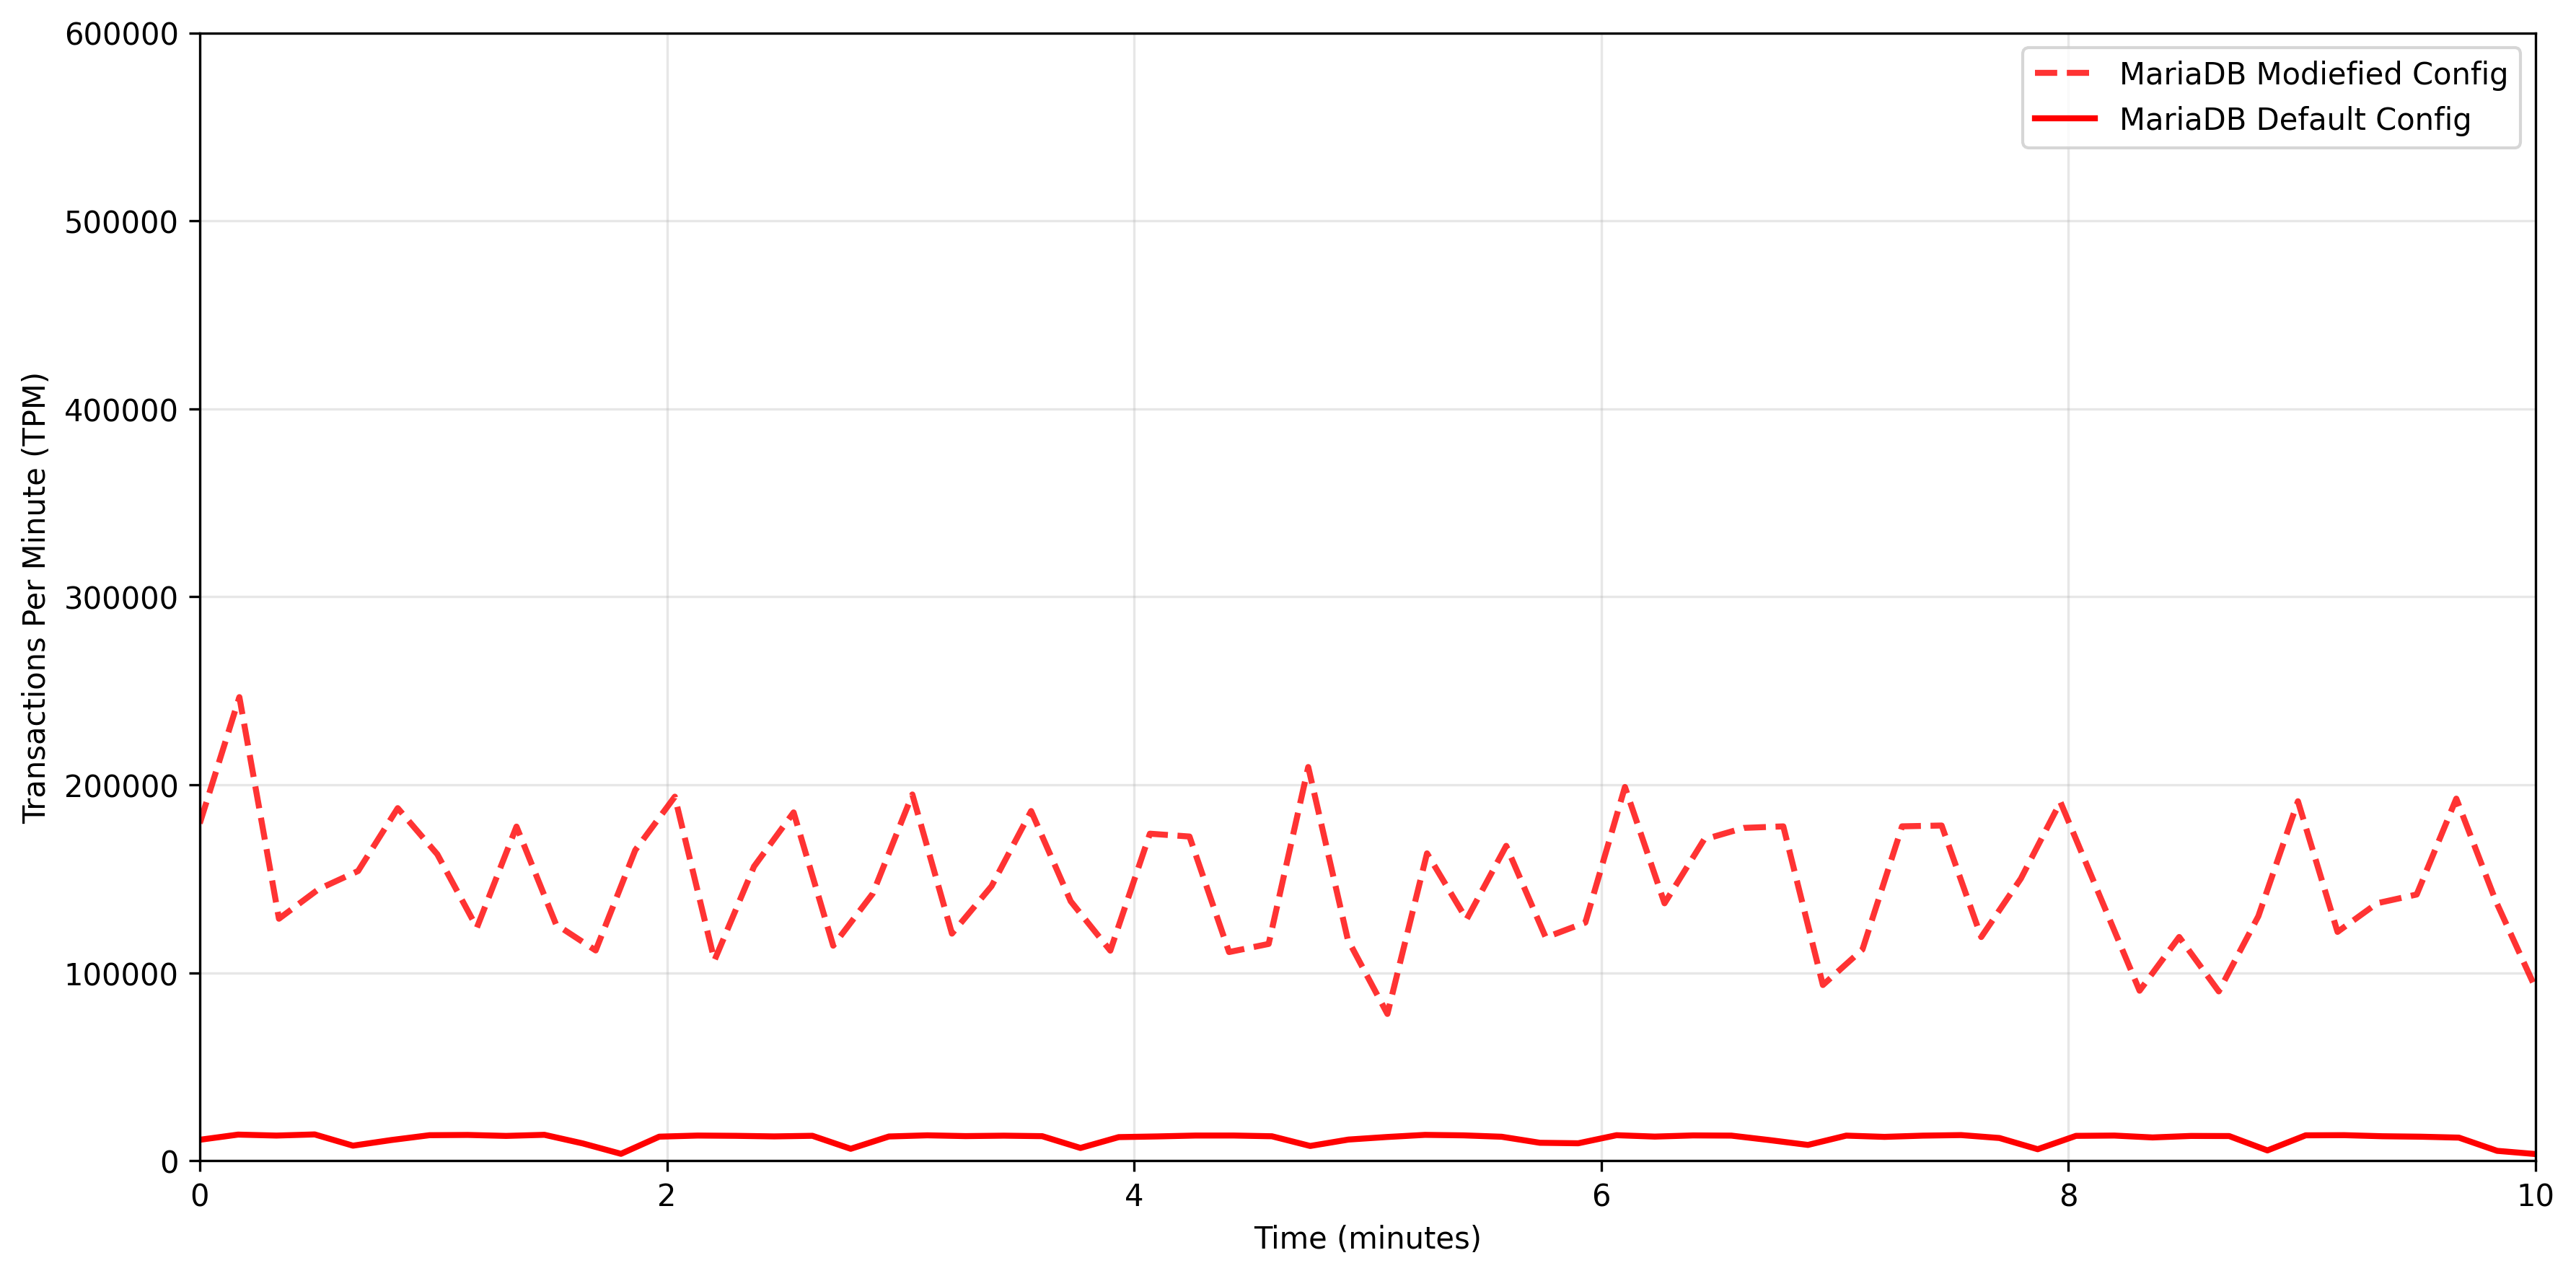
\includegraphics[width=\linewidth]{Images/dcnf_database_count_comparison_MariaDB.png}
        \caption{Impact of Configuration on MariaDB (TPM)}
        \label{fig:mariadb-dcnf}
    \end{subfigure}%
    \begin{subfigure}[b]{0.6\textwidth}
        \centering
        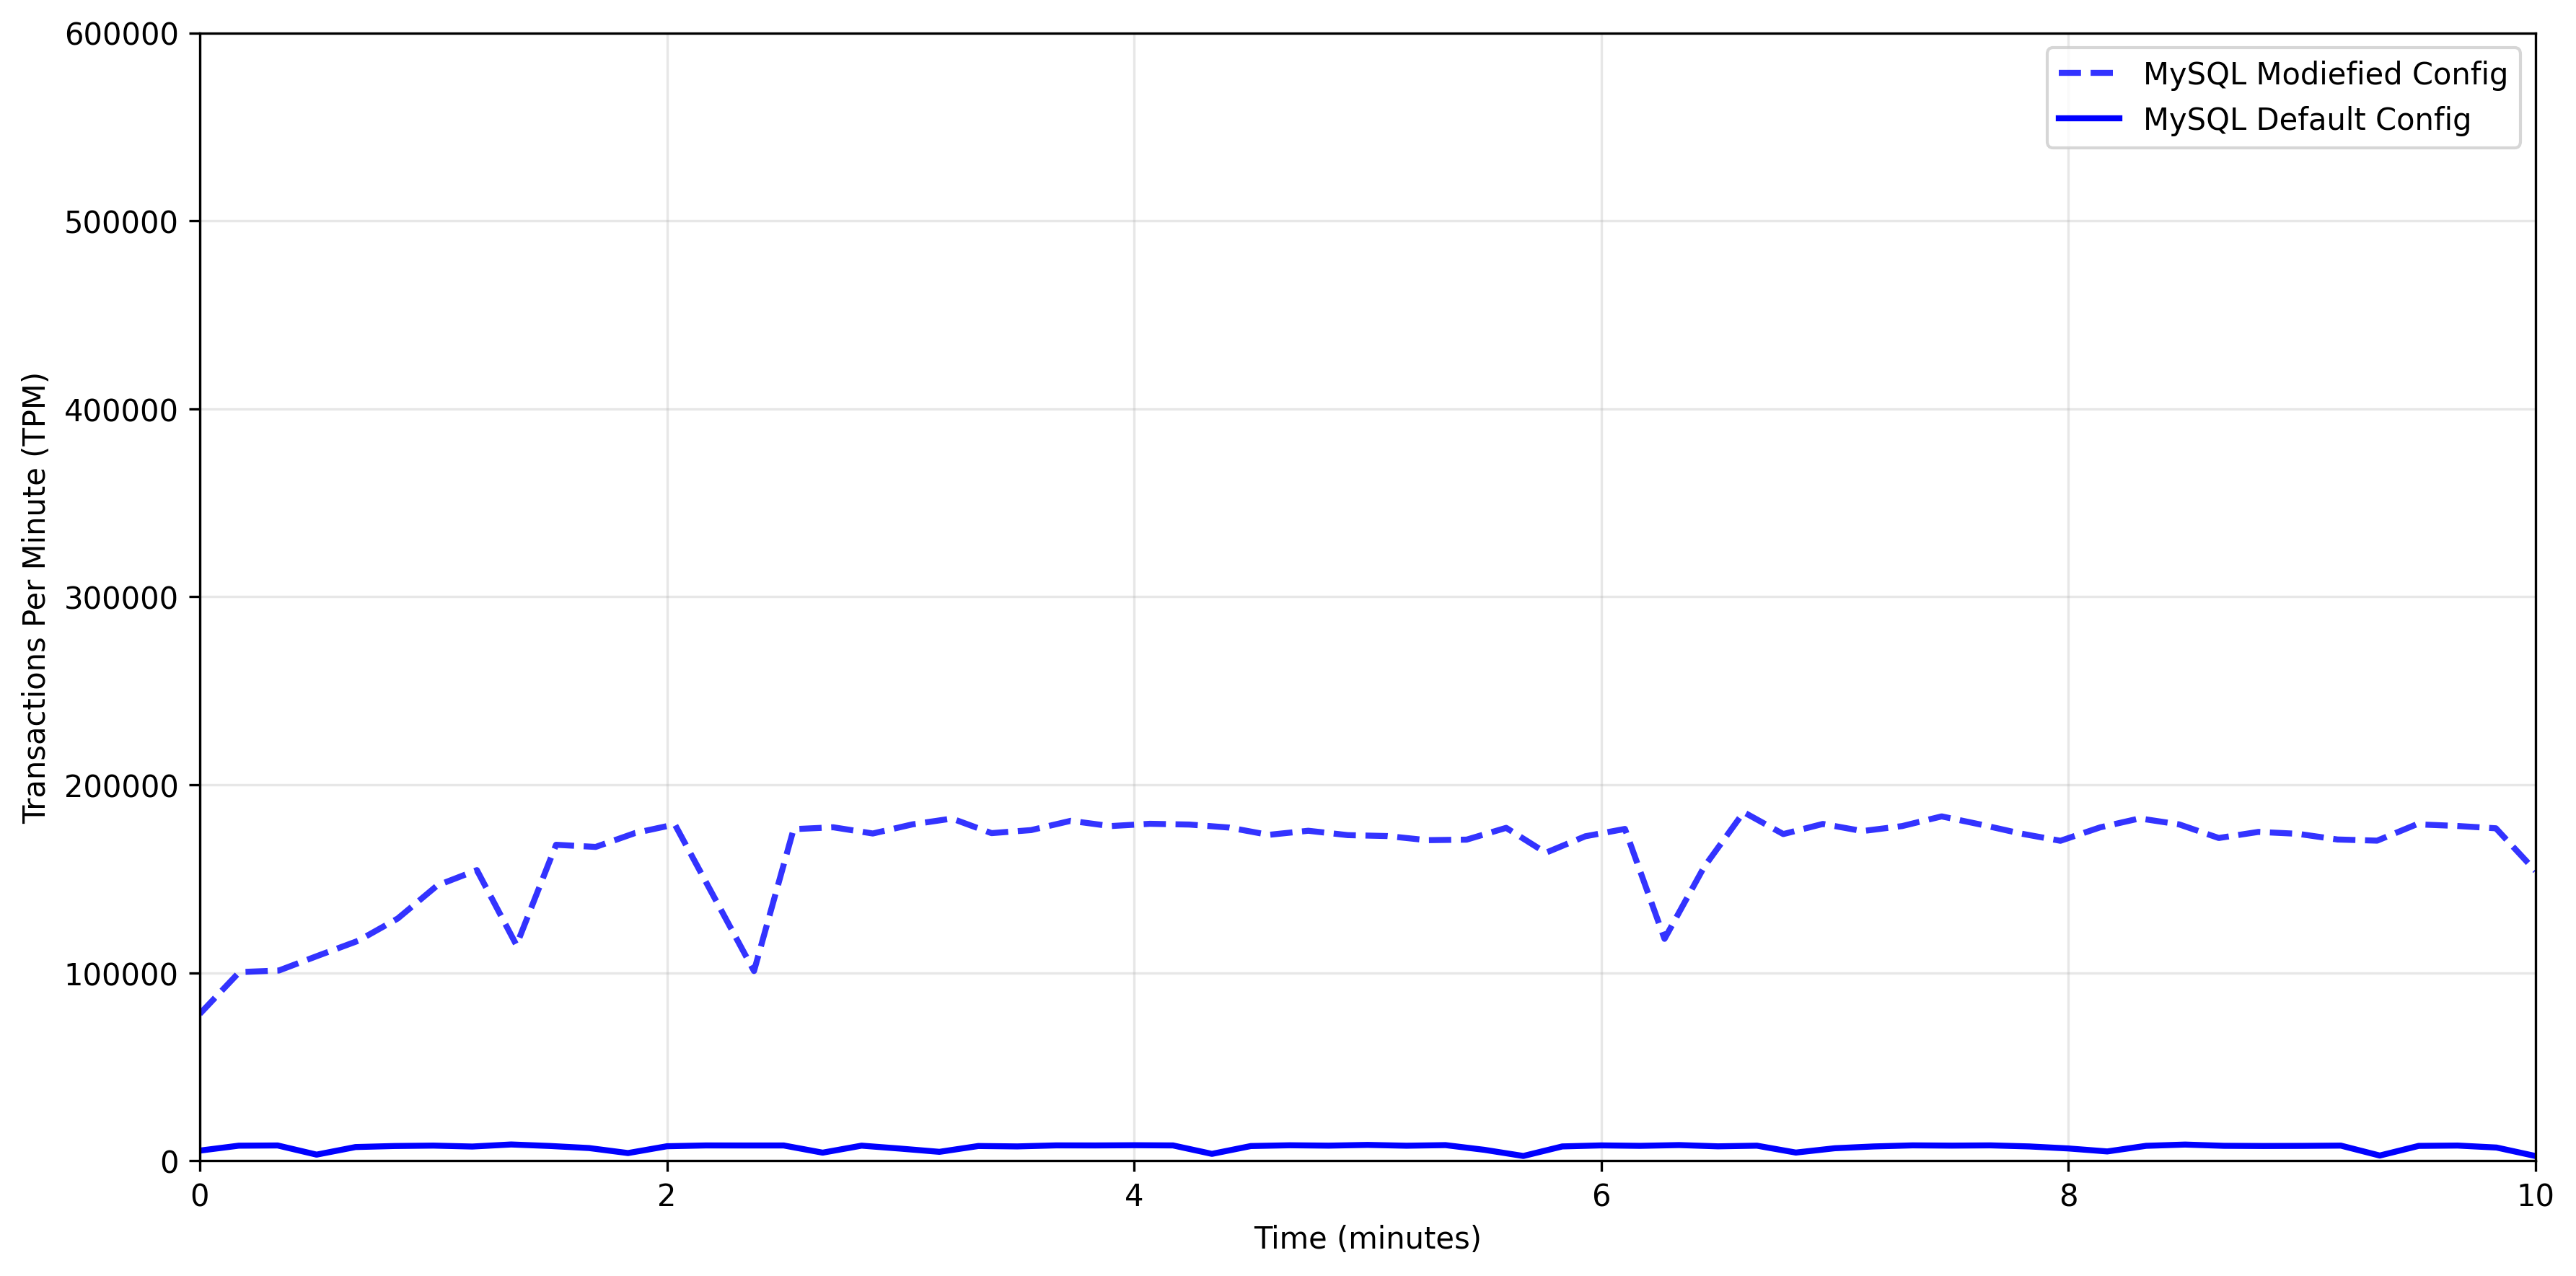
\includegraphics[width=\linewidth]{Images/dcnf_database_count_comparison_MySQL.png}
        \caption{Impact of Configuration on MySQL (TPM)}
        \label{fig:mysql-dcnf}
    \end{subfigure}

    \vspace{0.5cm}

    \hspace*{-1.7cm}
    \begin{subfigure}[b]{0.6\textwidth}
        \centering
        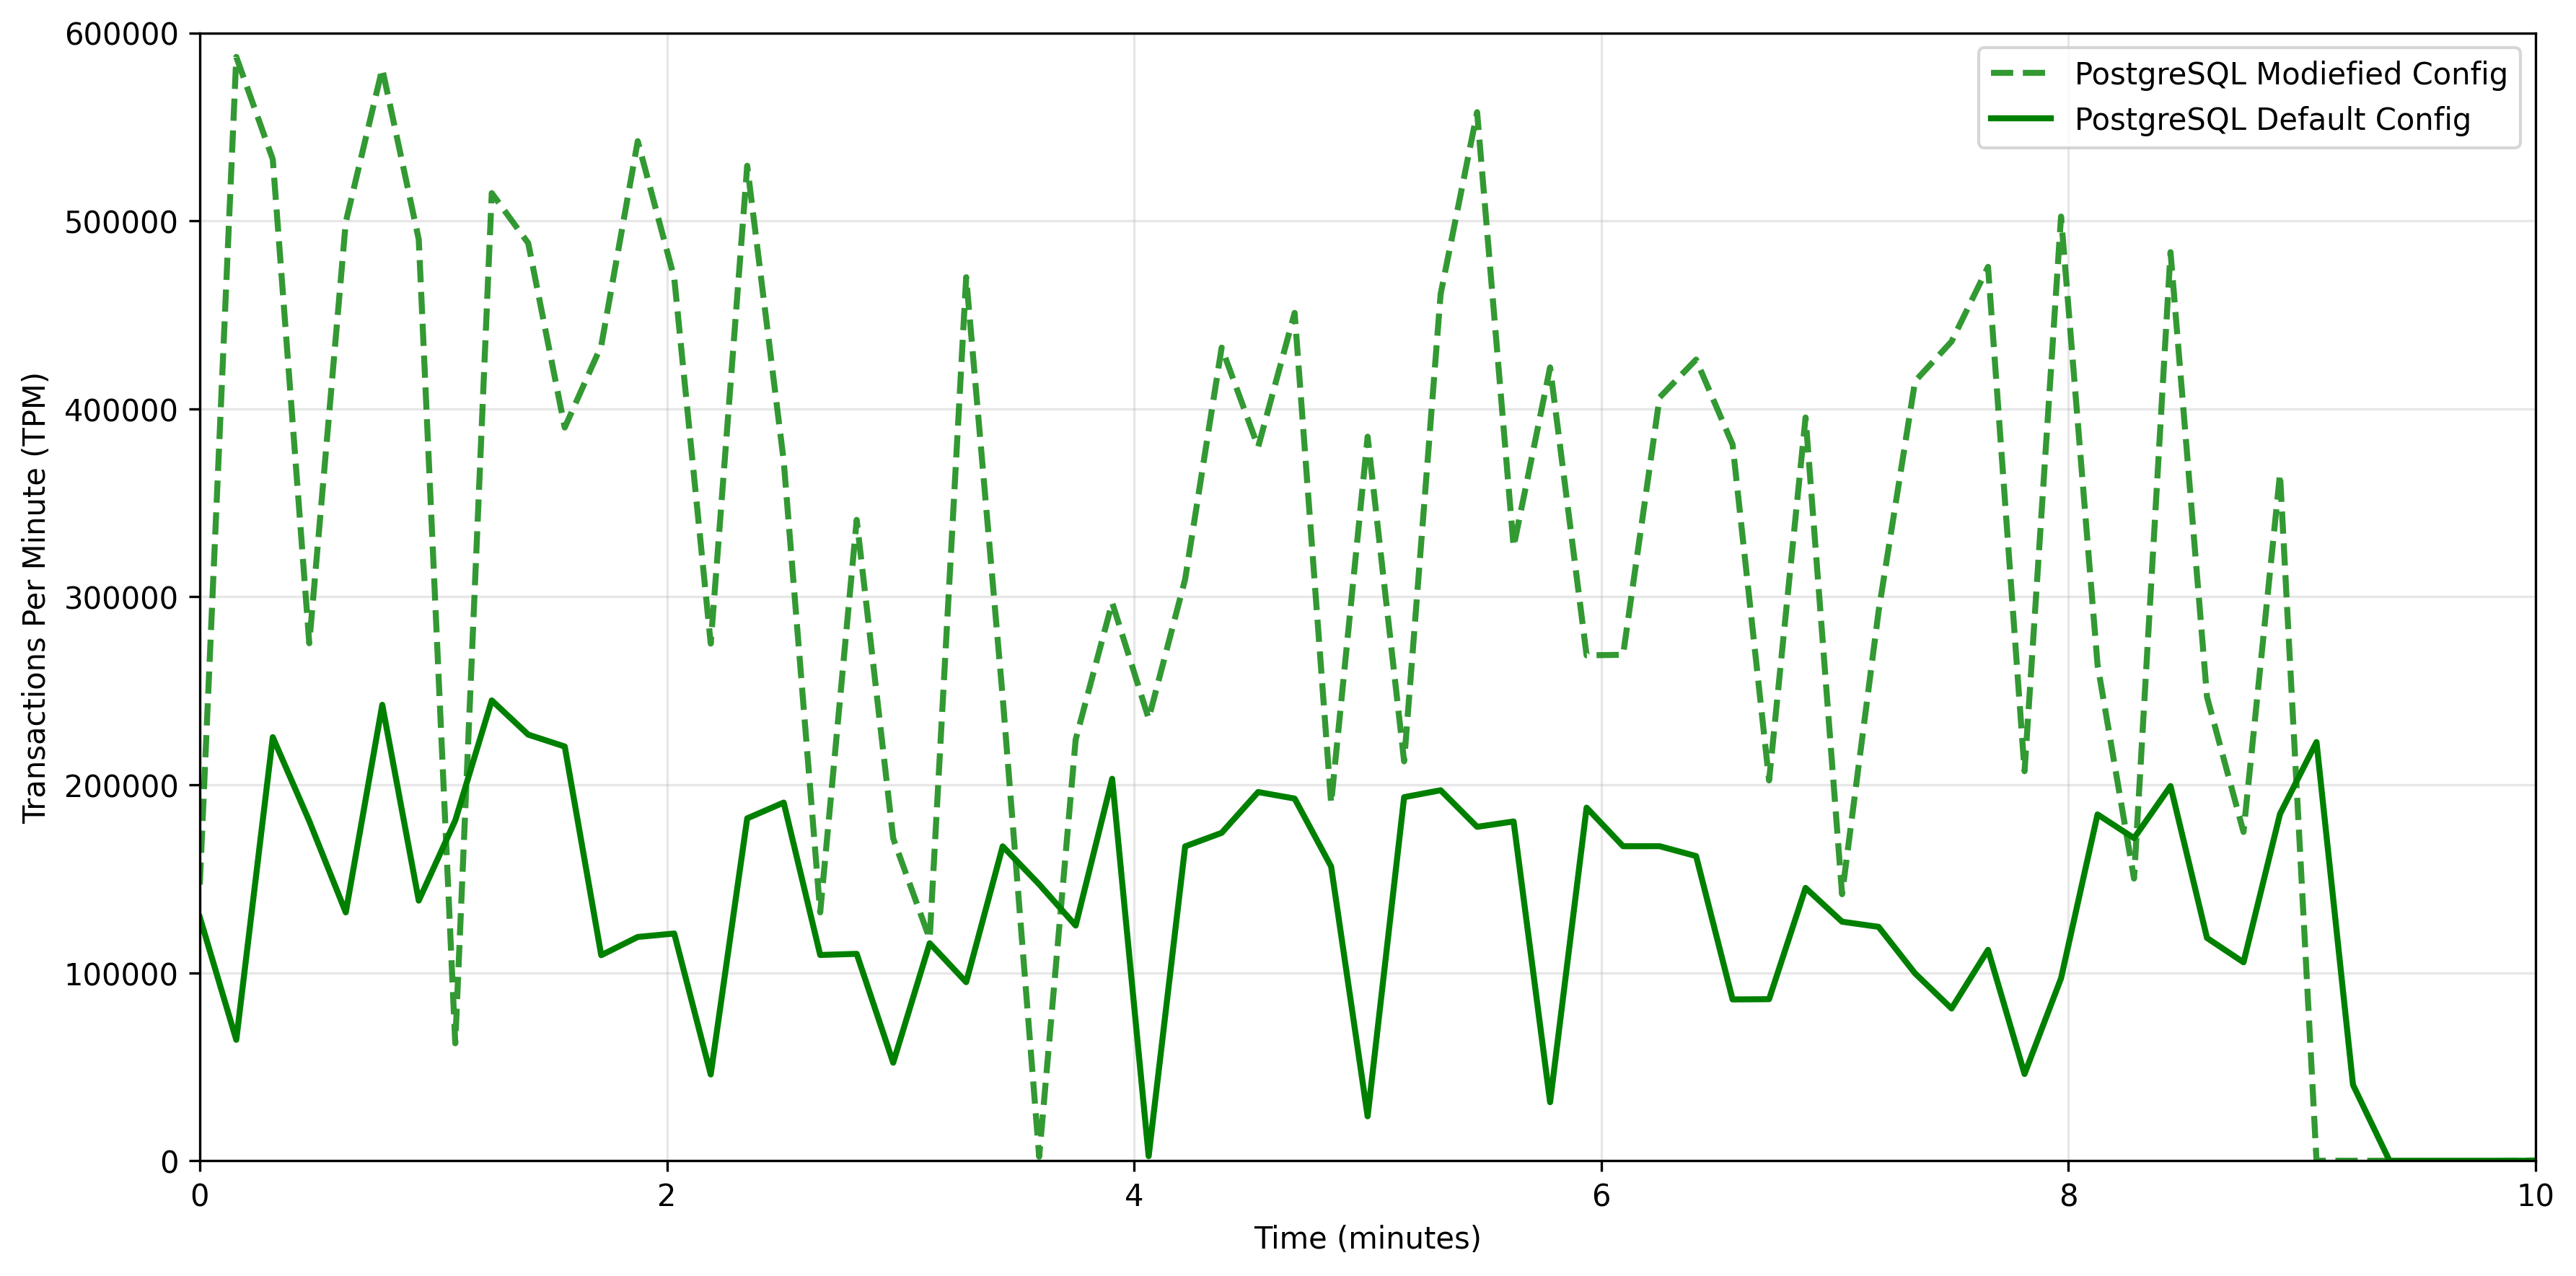
\includegraphics[width=\linewidth]{Images/dcnf_database_count_comparison_PostgreSQL.png}
        \caption{Impact of Configuration on PostgreSQL (TPM)}
        \label{fig:pg-dcnf}
    \end{subfigure}%
    \begin{subfigure}[b]{0.6\textwidth}
        \centering
        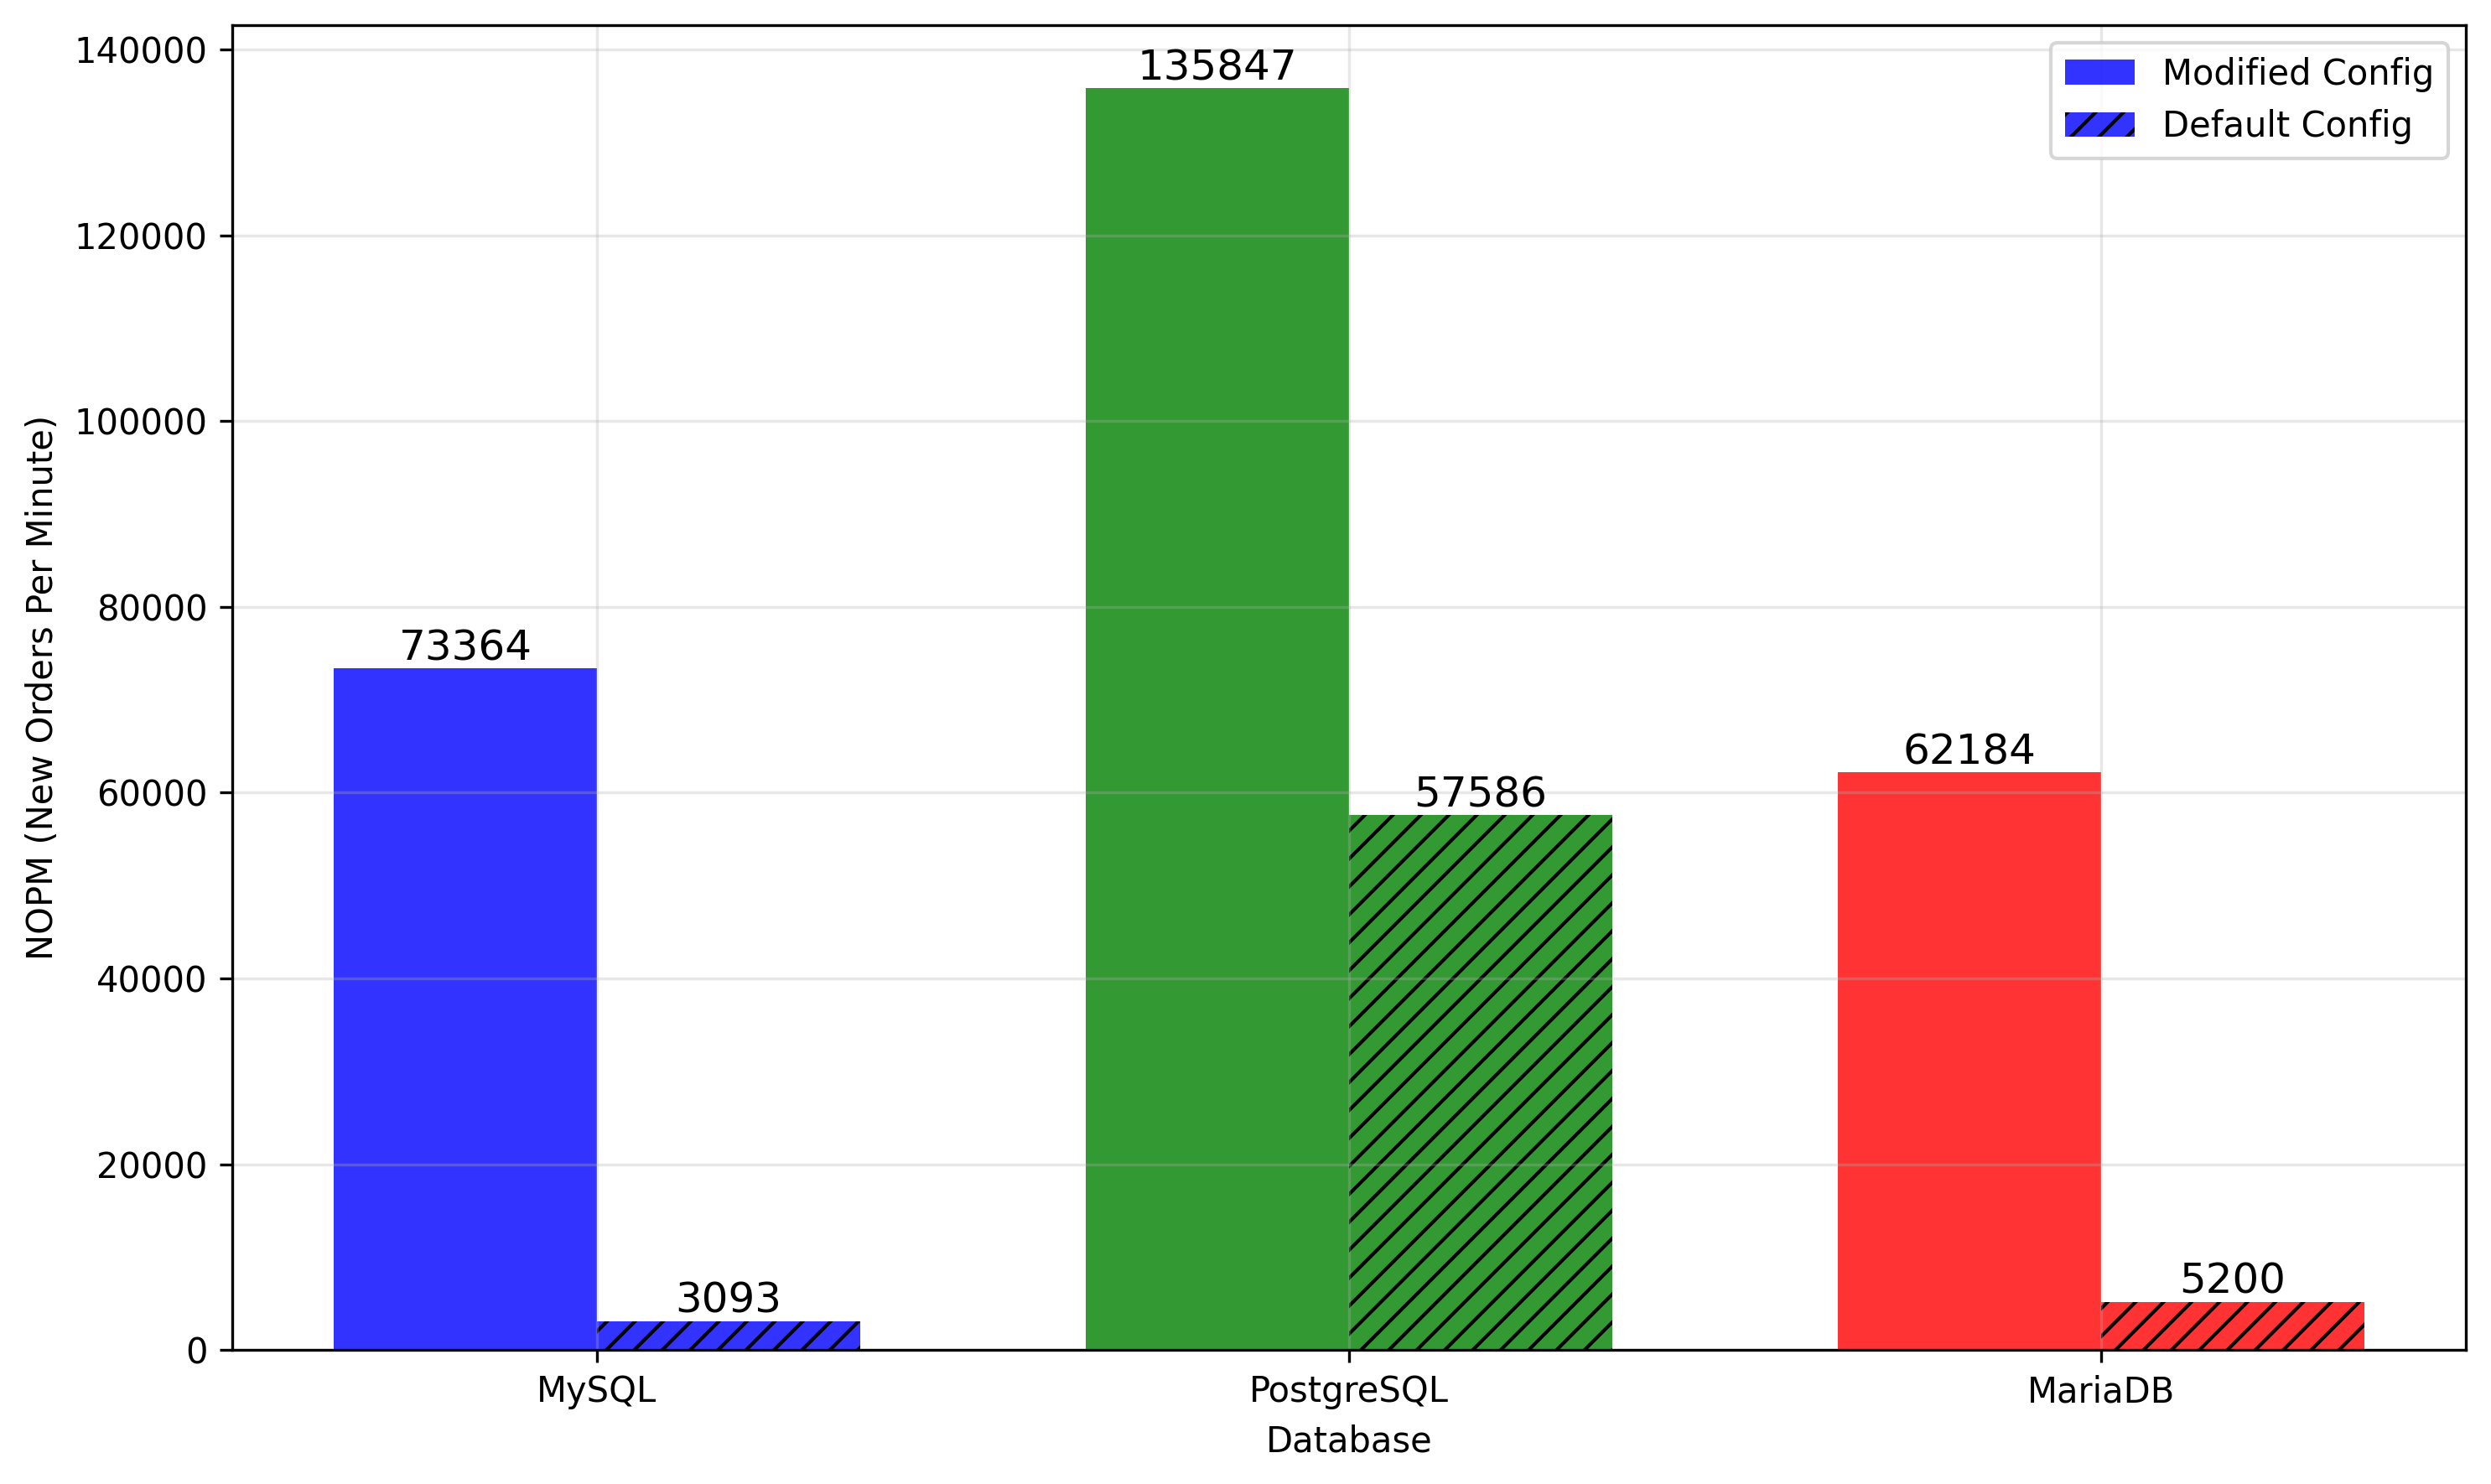
\includegraphics[width=\linewidth]{Images/hammerdb_summary_comparison_dcnf.png}
        \caption{Impact of Configuration across all Databases (NOPM)}
        \label{fig:nopm-dcnf}
    \end{subfigure}

    \caption{Performance analysis of custom configurations for VU=12 and WH=60 on PC 1}
    \label{fig:dcnf-all}
    
\end{figure}

Figure \ref{fig:dcnf-all} compares the effect of tailored configuration parameters on the performance of three DBMS - MariaDB, MySQL and PostgreSQL - based on a controlled load setting: 12 virtual users (VUs) and 60 warehouses, executed on \textbf{PC1}.

\begin{itemize}
    \setlength\itemsep{0.1em}
    \item \textbf{MariaDB (Figure \ref{fig:mariadb-dcnf}):} On average, it achieved a TPM comparable to MySQL, though with slightly less stability, which resulted on a lesser total number of transactions. The results with the default configuration were unexpectedly low, which we suspect is largely due to the small InnoDB buffer pool size in the default settings (128 MB). Nevertheless, the performance improvement brought by the configuration is remarkable, increasing the results by several factors.
    \item \textbf{MySQL (Figure \ref{fig:mysql-dcnf}):} Recorded a high total TPM, indicating greater usage of the modified installation. Although its default configuration performed worse than that of MariaDB, the InnoDB engine in MySQL appears to benefit more from tuning. However, the final results are quite similar, with differences falling within the expected standard deviation.
    \newpage
    \item \textbf{PostgreSQL (Figure \ref{fig:pg-dcnf}):} The biggest surprise of these tests was PostgreSQL's performance, which, on average, doubled the TPM results of both MySQL and MariaDB. Despite high fluctuations in throughput, PostgreSQL clearly outperformed the others. Even when comparing the NOPM results[\ref{fig:nopm-dcnf}] with its default configuration, it managed to only achieve results 10–20\% lower than the tuned versions of MariaDB and MySQL, respectively. This outcome was highly unexpected. After multiple reruns and thorough verification of the test environments and configurations, we attribute this advantage primarily to PostgreSQL's Multiversion Concurrency Control (MVCC) architecture, which handles concurrent transactions more efficiently, and its superior query planner, which often generates more optimized execution paths. 
\end{itemize}

\textbf{Conclusion:} The benchmark executed on \textbf{\hyperref[tab:hardware-setup]{PC 1}} shows that MySQL and MariaDB benefit significantly from configuration tuning, even though they are still outperformed by PostgreSQL in both TPM and NOPM. As it stands, PostgreSQL appears to be the clear leader in performance by a substantial margin. To ensure that this result is not due to a software or hardware issue specific to PC 1, we will next evaluate how each database performs with its modified configuration across all machine setups.

\subsection{Performance along the different Machines}

This chapter provides TPM (Transations Per Minute) performance for MariaDB, MySQL and PostgreSQL under four concurrency levels: 2, 4, 8 and 12 Virtual Users (VUs). The goal is to see how well each DBMS scales to higher concurrency and workload intensity for the four computers.

\subsubsection{MariaDB}

\begin{figure}[H]
    \centering
    \hspace*{-1.7cm}
    \begin{subfigure}[b]{0.6\textwidth}
        \centering
        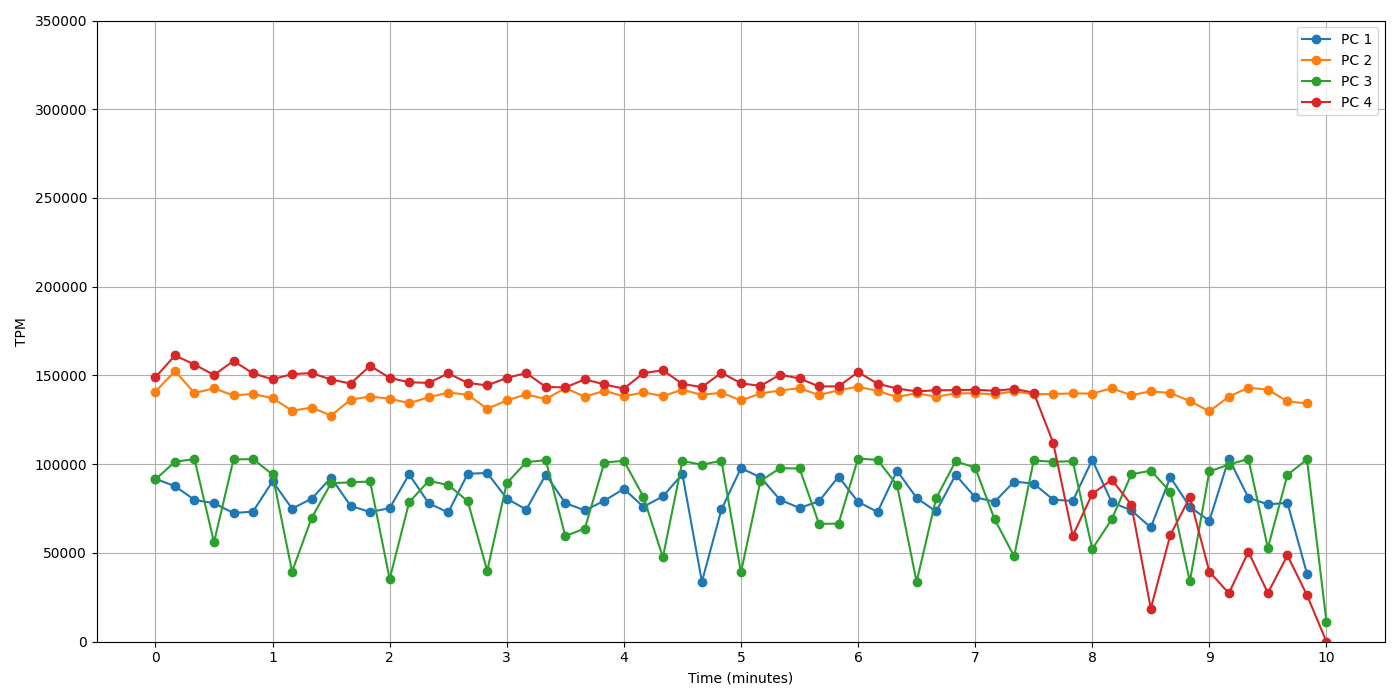
\includegraphics[width=\linewidth]{Images/hdbtcount_MariaDB_2.png}
        \caption{MariaDB with 2 Virtual Users}
        \label{fig:mariadb-2vu}
    \end{subfigure}%
    \begin{subfigure}[b]{0.6\textwidth}
        \centering
        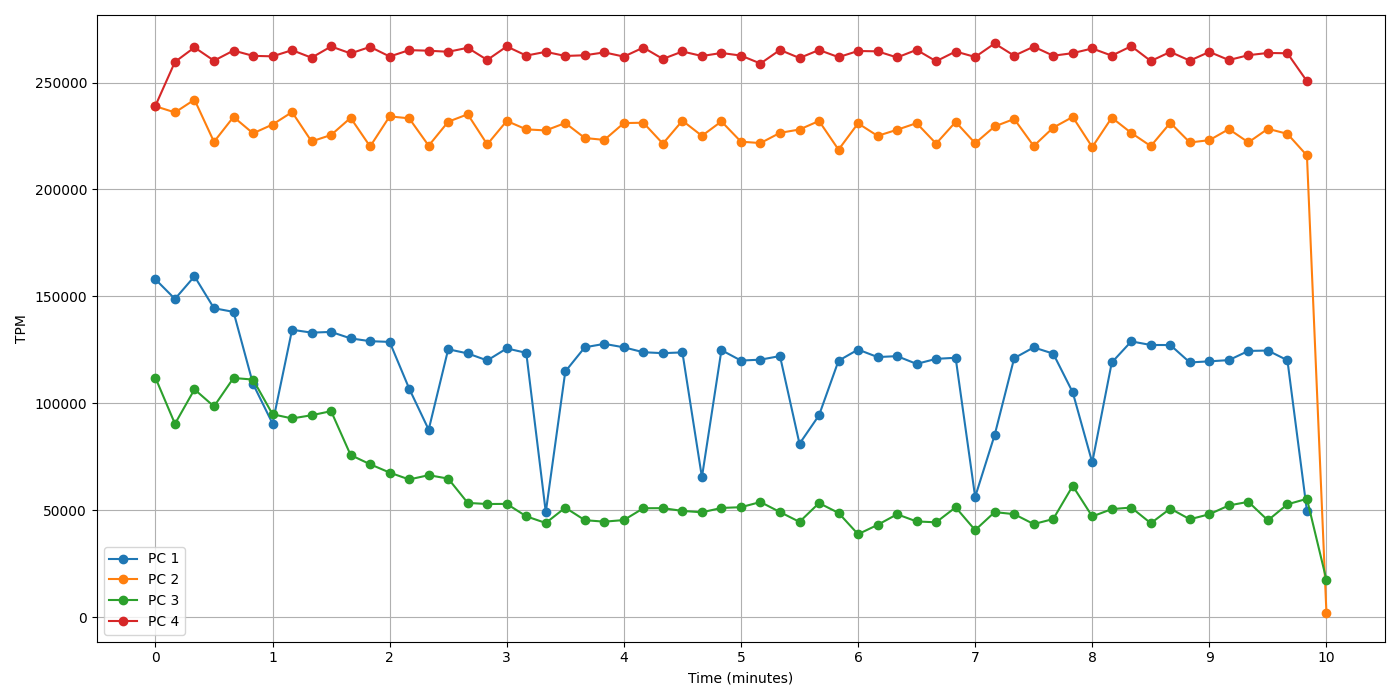
\includegraphics[width=\linewidth]{Images/hdbtcount_MariaDB_4.png}
        \caption{MariaDB with 4 Virtual Users}
        \label{fig:mariadb-4vu}
    \end{subfigure}

    \vspace{0.5cm}

    \hspace*{-1.7cm}
    \begin{subfigure}[b]{0.6\textwidth}
        \centering
        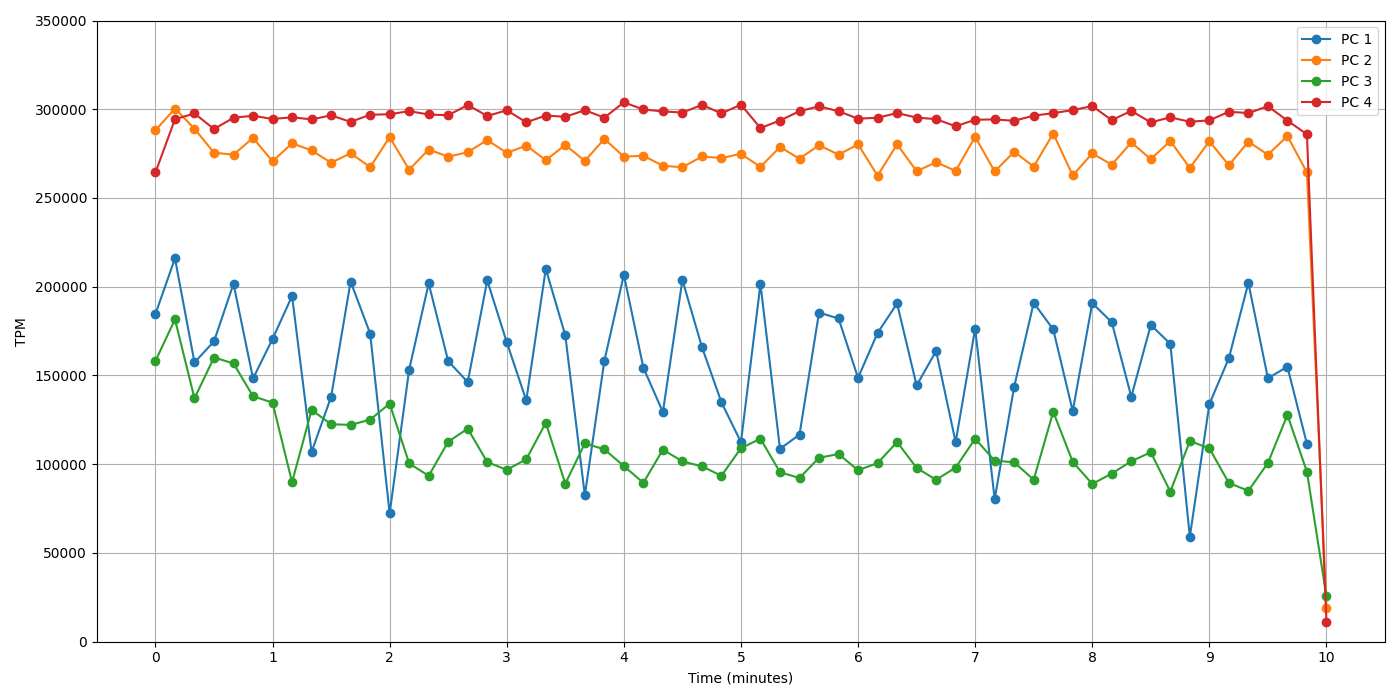
\includegraphics[width=\linewidth]{Images/hdbtcount_MariaDB_8.png}
        \caption{MariaDB with 8 Virtual Users}
        \label{fig:mariadb-8vu}
    \end{subfigure}%
    \begin{subfigure}[b]{0.6\textwidth}
        \centering
        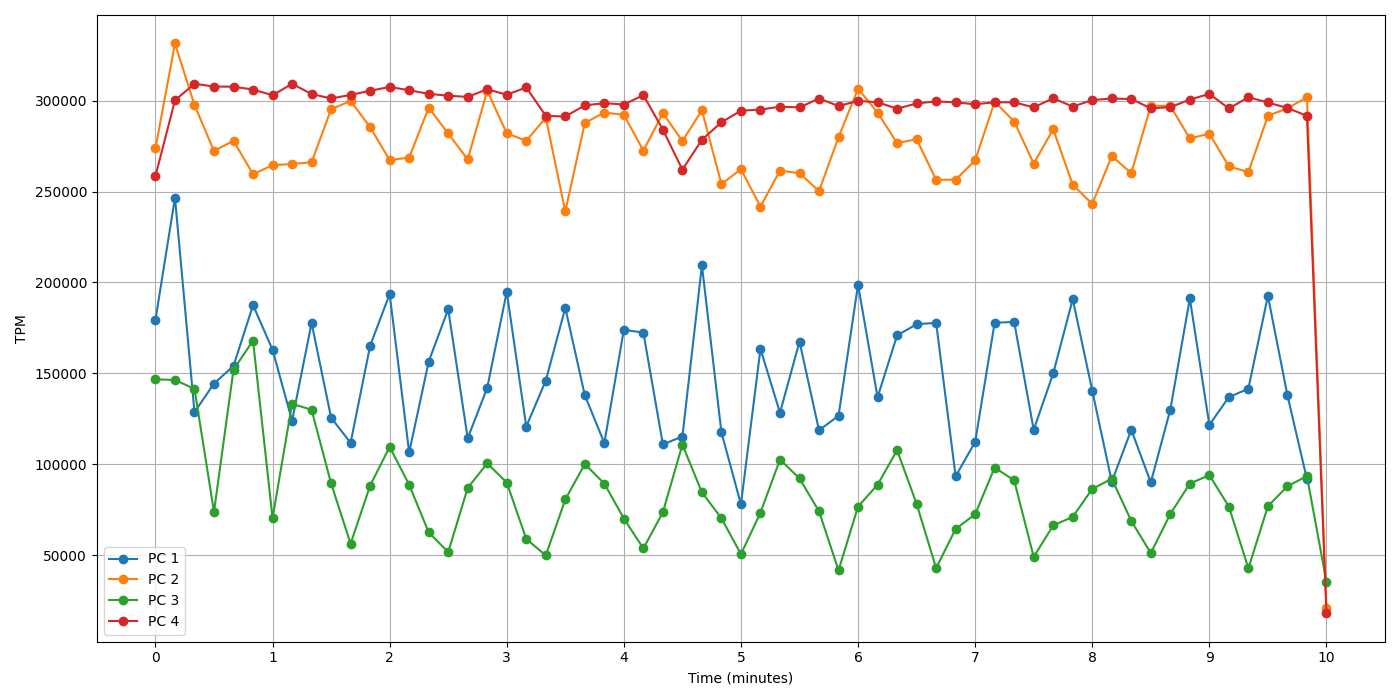
\includegraphics[width=\linewidth]{Images/hdbtcount_MariaDB_12.png}
        \caption{MariaDB with 12 Virtual Users}
        \label{fig:mariadb-12vu}
    \end{subfigure}

    \caption{Performance of MariaDB with different numbers of virtual users}
    \label{fig:mariadb-all}
\end{figure}

Figure \ref{fig:mariadb-all} shows that MariaDB exhibits stable behavior with the increase in virtual users:

\begin{itemize}
    \setlength\itemsep{0.1em}
    \item \textbf{2 to 4 VUs:} A modest TPM growth, showing that MariaDB is actually benefiting from medium concurrency.
    \item \textbf{8 VUs:} System begins to experience stress and TPM growth stabilizes or decreases to some extent.
    \item \textbf{12 VUs:} Performance is consistent but is demonstrating that it is reaching its peak. The results are very identical to the ones in 8 virtual users which indicates a possible bottleneck.
\end{itemize}

 Overall, MariaDB scales pretty well but with diminishing returns after 8 VUs. It's possible that it needs additional tuning or more sophisticated storage engines to scale adequately at even higher loads.

\subsubsection{MySQL}

\begin{figure}[H]
    \centering
    \hspace*{-1.7cm}
    \begin{subfigure}[b]{0.6\textwidth}
        \centering
        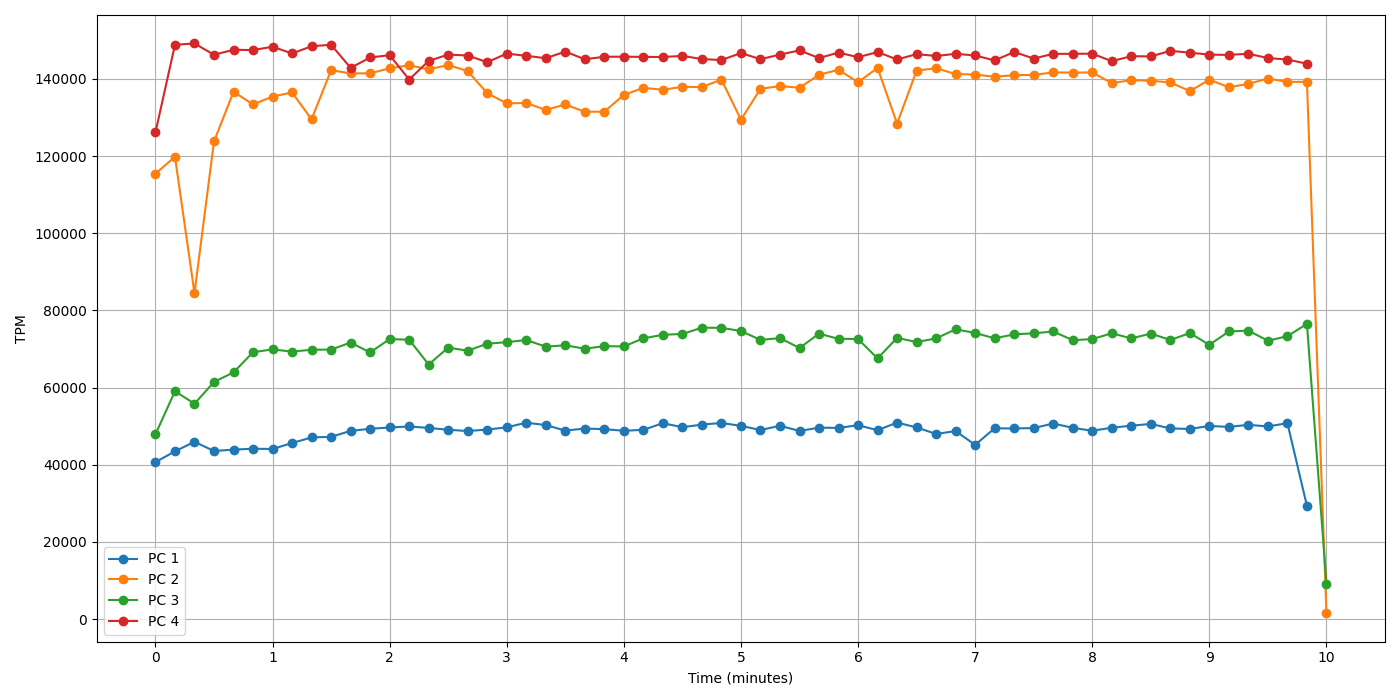
\includegraphics[width=\linewidth]{Images/hdbtcount_MySQL_2.png}
        \caption{MySQL with 2 Virtual Users}
        \label{fig:mysql-2vu}
    \end{subfigure}%
    \begin{subfigure}[b]{0.6\textwidth}
        \centering
        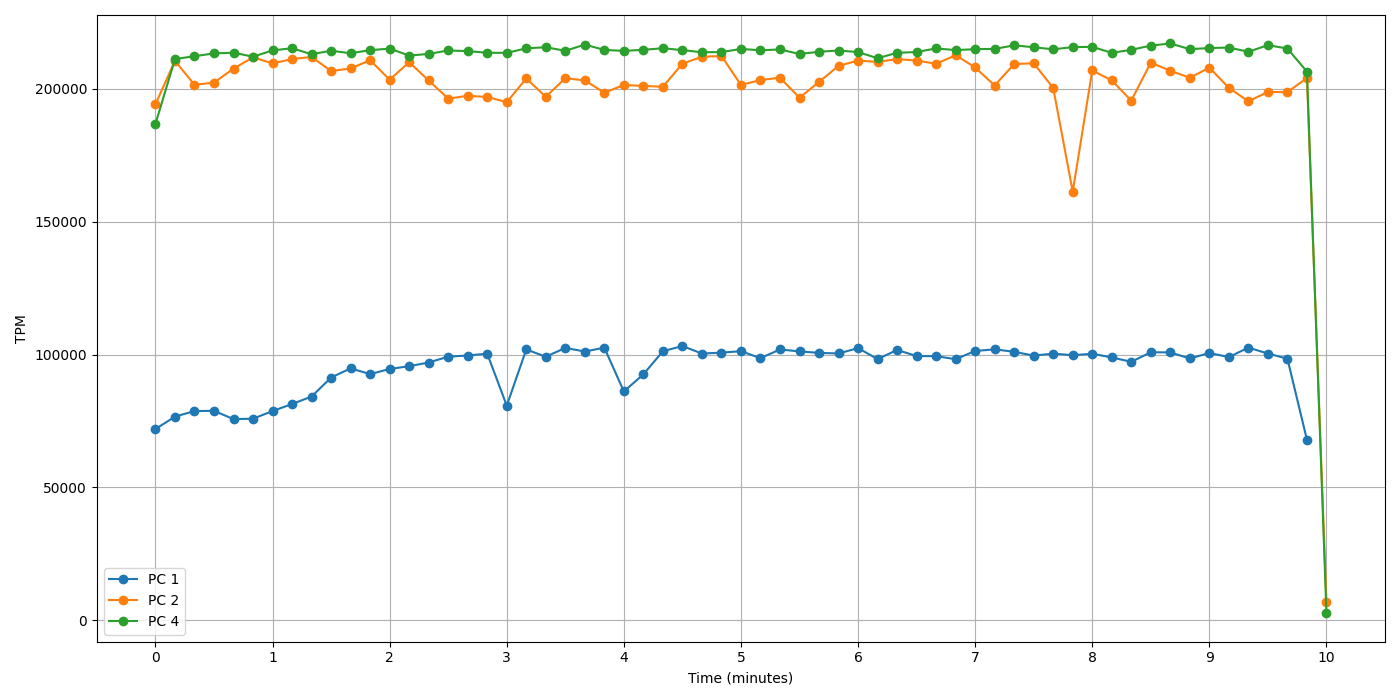
\includegraphics[width=\linewidth]{Images/hdbtcount_MySQL_4.png}
        \caption{MySQL with 4 Virtual Users}
        \label{fig:mysql-4vu}
    \end{subfigure}

    \vspace{0.5cm}

    \hspace*{-1.7cm}
    \begin{subfigure}[b]{0.6\textwidth}
        \centering
        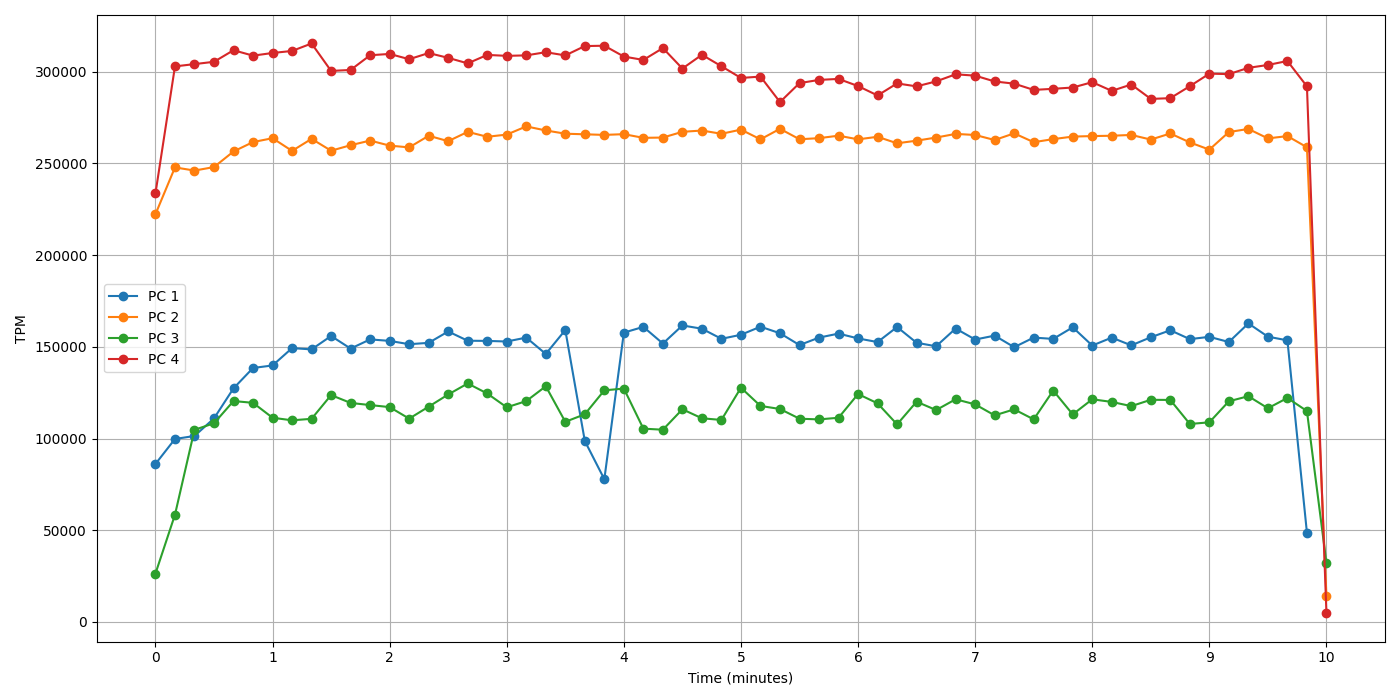
\includegraphics[width=\linewidth]{Images/hdbtcount_MySQL_8.png}
        \caption{MySQL with 8 Virtual Users}
        \label{fig:mysql-8vu}
    \end{subfigure}%
    \begin{subfigure}[b]{0.6\textwidth}
        \centering
        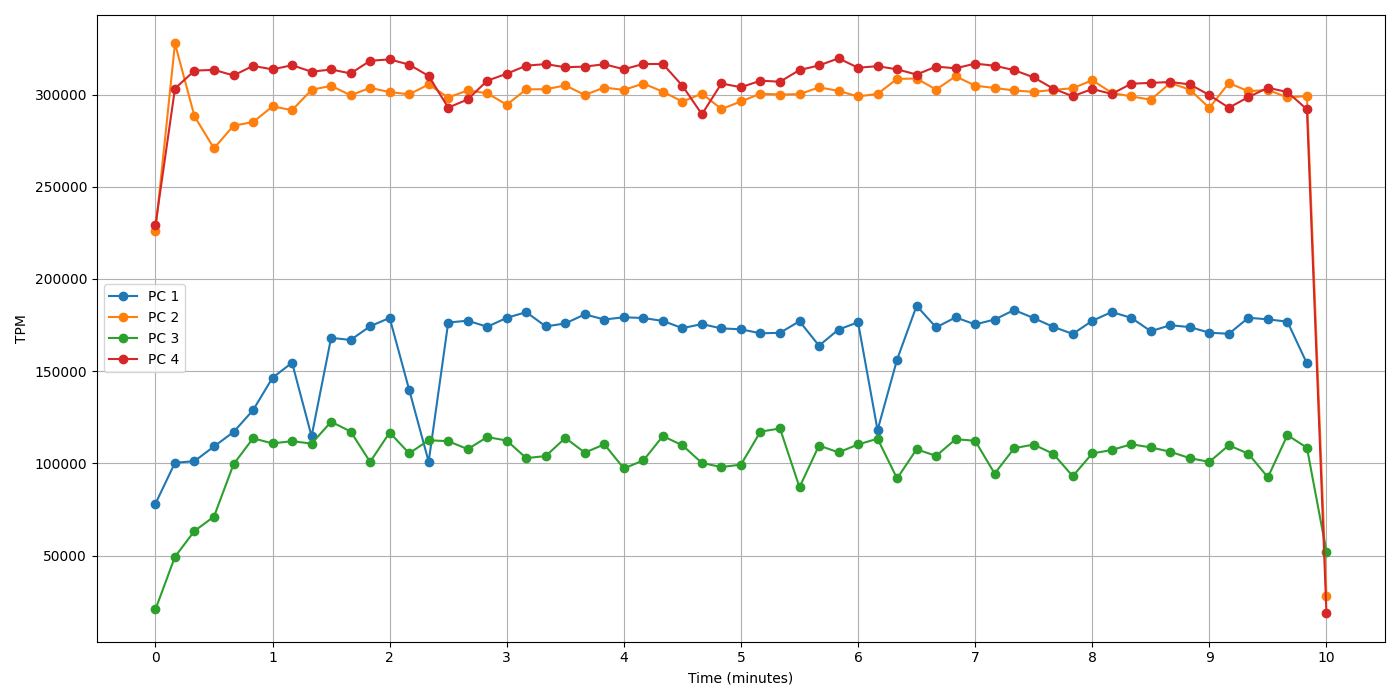
\includegraphics[width=\linewidth]{Images/hdbtcount_MySQL_12.png}
        \caption{MySQL with 12 Virtual Users}
        \label{fig:mysql-12vu}
    \end{subfigure}

    \caption{Performance of MySQL with different numbers of virtual users}
    \label{fig:mysql-all}
    
\end{figure}

Figure \ref{fig:mysql-all} shows a more responsive performance curve than MariaDB in some machines:

\begin{itemize}
    \setlength\itemsep{0.1em}
    \item \textbf{2 to 8 VUs:} Steady linear growth in TPM. The InnoDB engine handles increasing concurrency well.
    \item \textbf{12 VUs:} There are better results and stability in all machines compared to MariaDB.
\end{itemize}

MySQL shows good scalability and concurrency support. It is highly suitable for high-throughput OLTP workloads up to a moderate level of concurrency.

\subsubsection{PostgreSQL}

\begin{figure}[H]
    \centering
    \hspace*{-1.7cm}
    \begin{subfigure}[b]{0.6\textwidth}
        \centering
        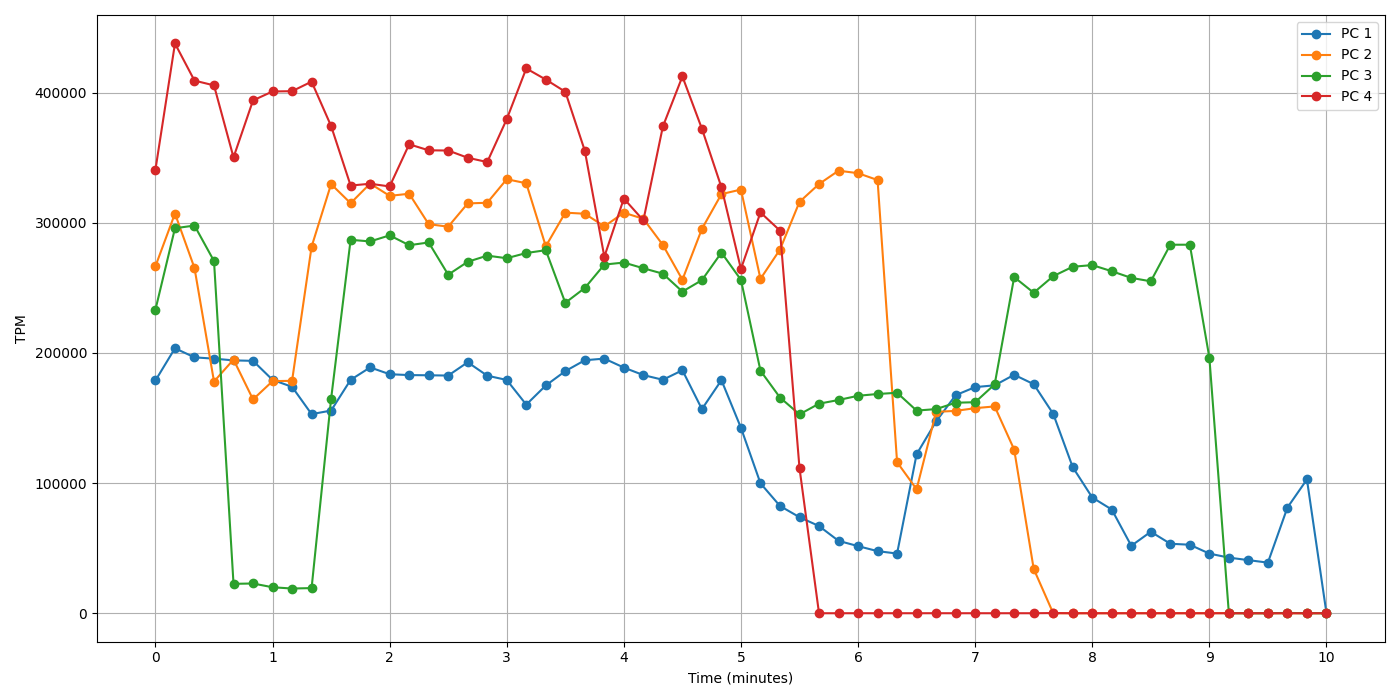
\includegraphics[width=\linewidth]{Images/hdbtcount_PostgreSQL_2.png}
        \caption{PostgreSQL with 2 Virtual Users}
        \label{fig:postgresql-2vu}
    \end{subfigure}%
    \begin{subfigure}[b]{0.6\textwidth}
        \centering
        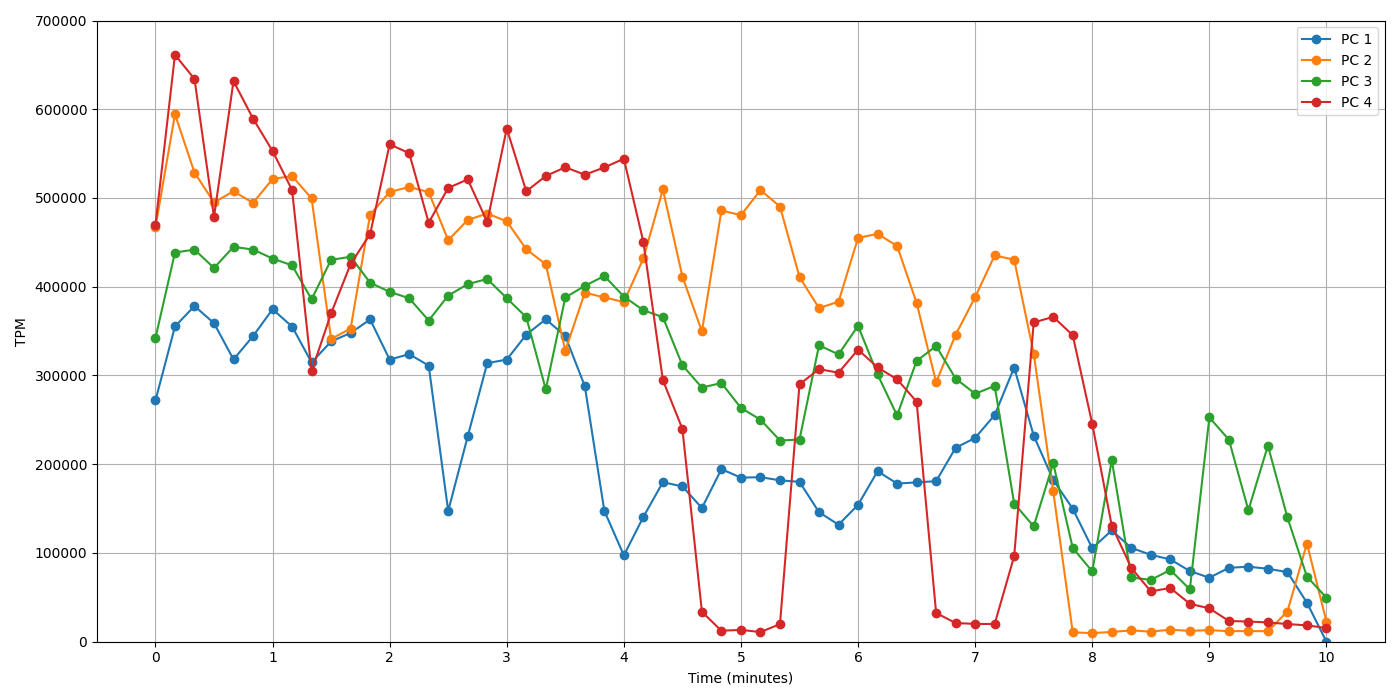
\includegraphics[width=\linewidth]{Images/hdbtcount_PostgreSQL_4.png}
        \caption{PostgreSQL with 4 Virtual Users}
        \label{fig:postgresql-4vu}
    \end{subfigure}

    \vspace{0.5cm}

    \hspace*{-1.7cm}
    \begin{subfigure}[b]{0.6\textwidth}
        \centering
        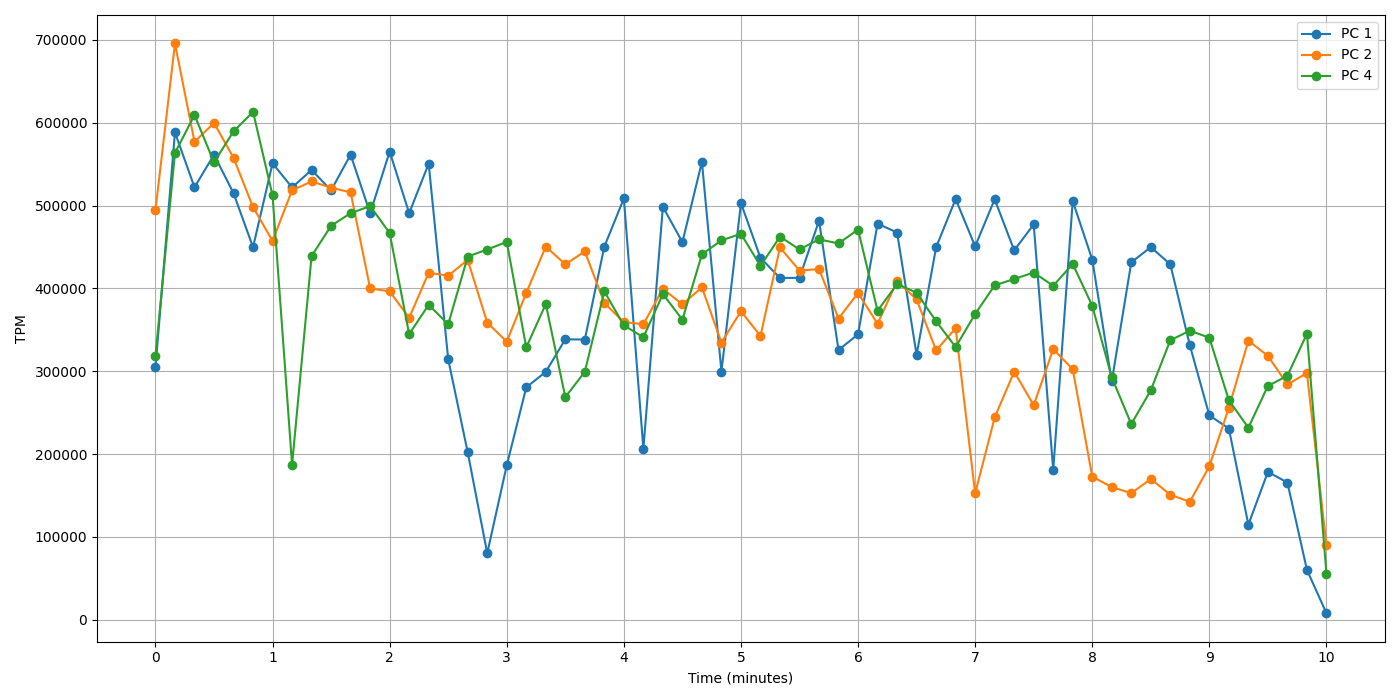
\includegraphics[width=\linewidth]{Images/hdbtcount_PostgreSQL_8.png}
        \caption{PostgreSQL with 8 Virtual Users}
        \label{fig:postgresql-8vu}
    \end{subfigure}%
    \begin{subfigure}[b]{0.6\textwidth}
        \centering
        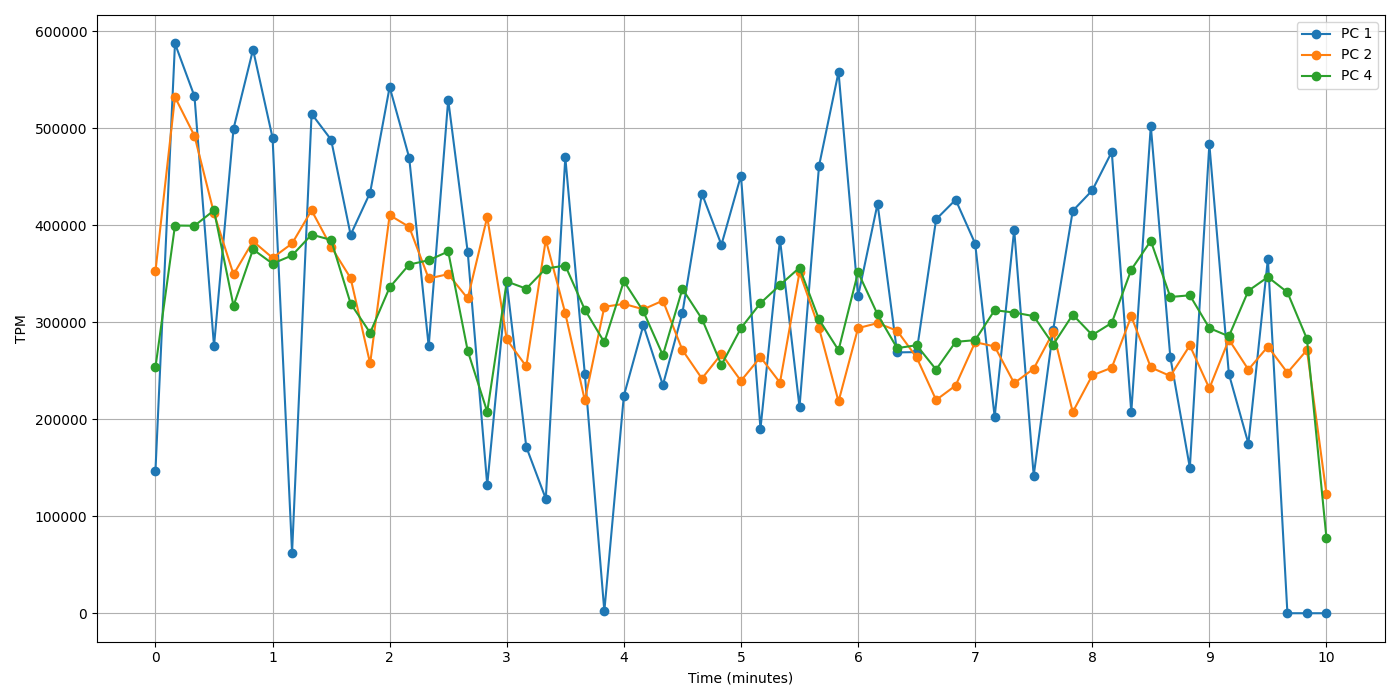
\includegraphics[width=\linewidth]{Images/hdbtcount_PostgreSQL_12.png}
        \caption{PostgreSQL with 12 Virtual Users}
        \label{fig:postgresql-12vu}
    \end{subfigure}

    \caption{Performance of PostgreSQL with different numbers of virtual users}
    \label{fig:postgresql-all}
    
\end{figure}

Figure \ref{fig:postgresql-all} confirms PostgreSQL's reputation for dealing with concurrency very well:

\begin{itemize}
    \setlength\itemsep{0.1em}
    \item \textbf{2 to 8 VUs:} TPM rises steadily and markedly, with great use of existing threads and MVCC.
    \item \textbf{12 VUs:} PostgreSQL still scales, holding or even increasing throughput to some extent in some machines, with little sign of performance degradation.
\end{itemize}

In general, PostgreSQL is the most scalable DBMS here. Its architecture (MVCC, indexing, planner) allows it to preserve high performance at high load, which prepares it for highly concurrent environments.

\vspace{2cm}

\subsubsection{Summarize}

We initially expected \hyperref[tab:hardware-setup]{PC 2} to be the top performer. However, somewhat surprisingly, \hyperref[tab:hardware-setup]{PC 4} slightly outperformed it, despite running HammerDB under an x86\_64 emulation layer on ARM64. On the other hand, \hyperref[tab:hardware-setup]{PC 1}, which is the only machine running on bare metal, was among the worst performers—only consistently outperforming \hyperref[tab:hardware-setup]{PC 3} in MySQL and MariaDB tests, while showing mixed results in PostgreSQL. These findings suggest that disk speed may be the key performance factor in this setup. \hyperref[tab:hardware-setup]{PC 1} uses the oldest and slowest disk, while \hyperref[tab:hardware-setup]{PC 2} and \hyperref[tab:hardware-setup]{PC 4} have similar storage performance despite different CPU architectures, what could explain the results. Meanwhile, despite having a fast SSD, \hyperref[tab:hardware-setup]{PC 3} has the weakest CPU among all machines, what could have dragged it down.

\subsection{Metrics of Different Machines}

\begin{figure}[H]
    \centering
    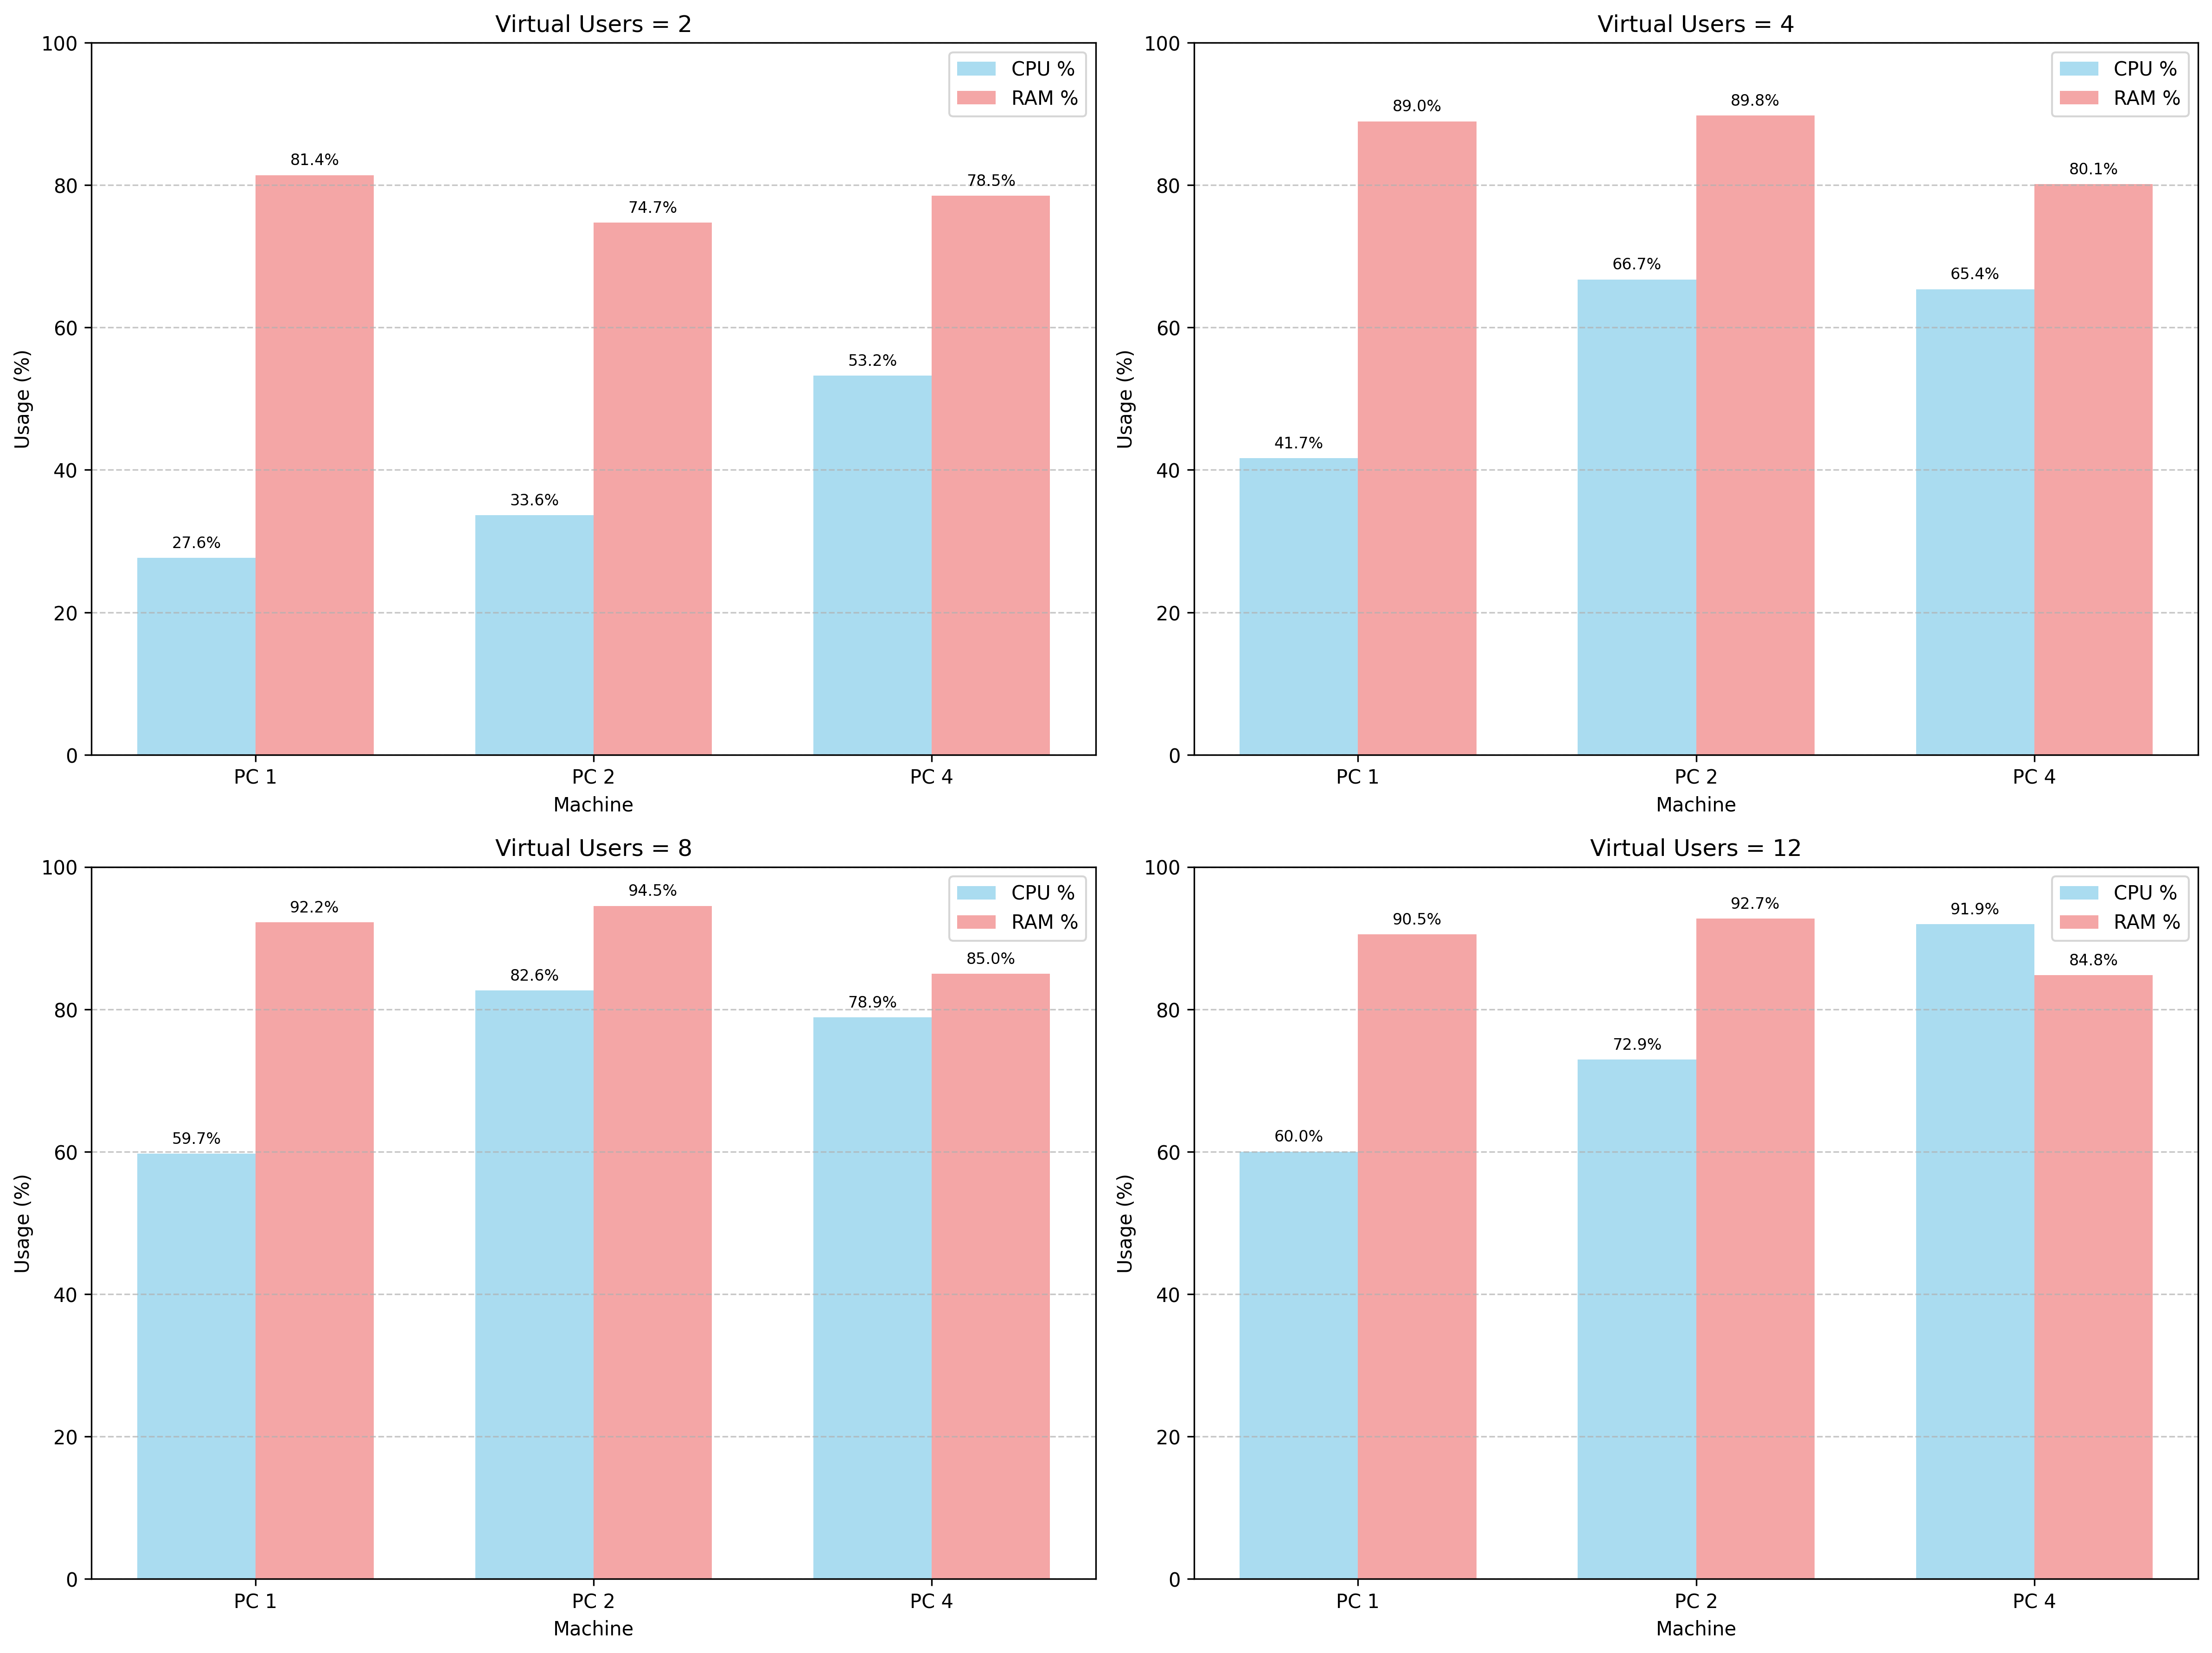
\includegraphics[width=0.87\linewidth]{Images/sys_usage_mariadb_time_ranges_filtered.png}
    \caption{CPU and RAM usage on all tests using MariaDB}
    \label{fig:mariadb-cpu-ram}
\end{figure}

    \vspace{0.5cm}

\begin{figure}[H]
    \centering
    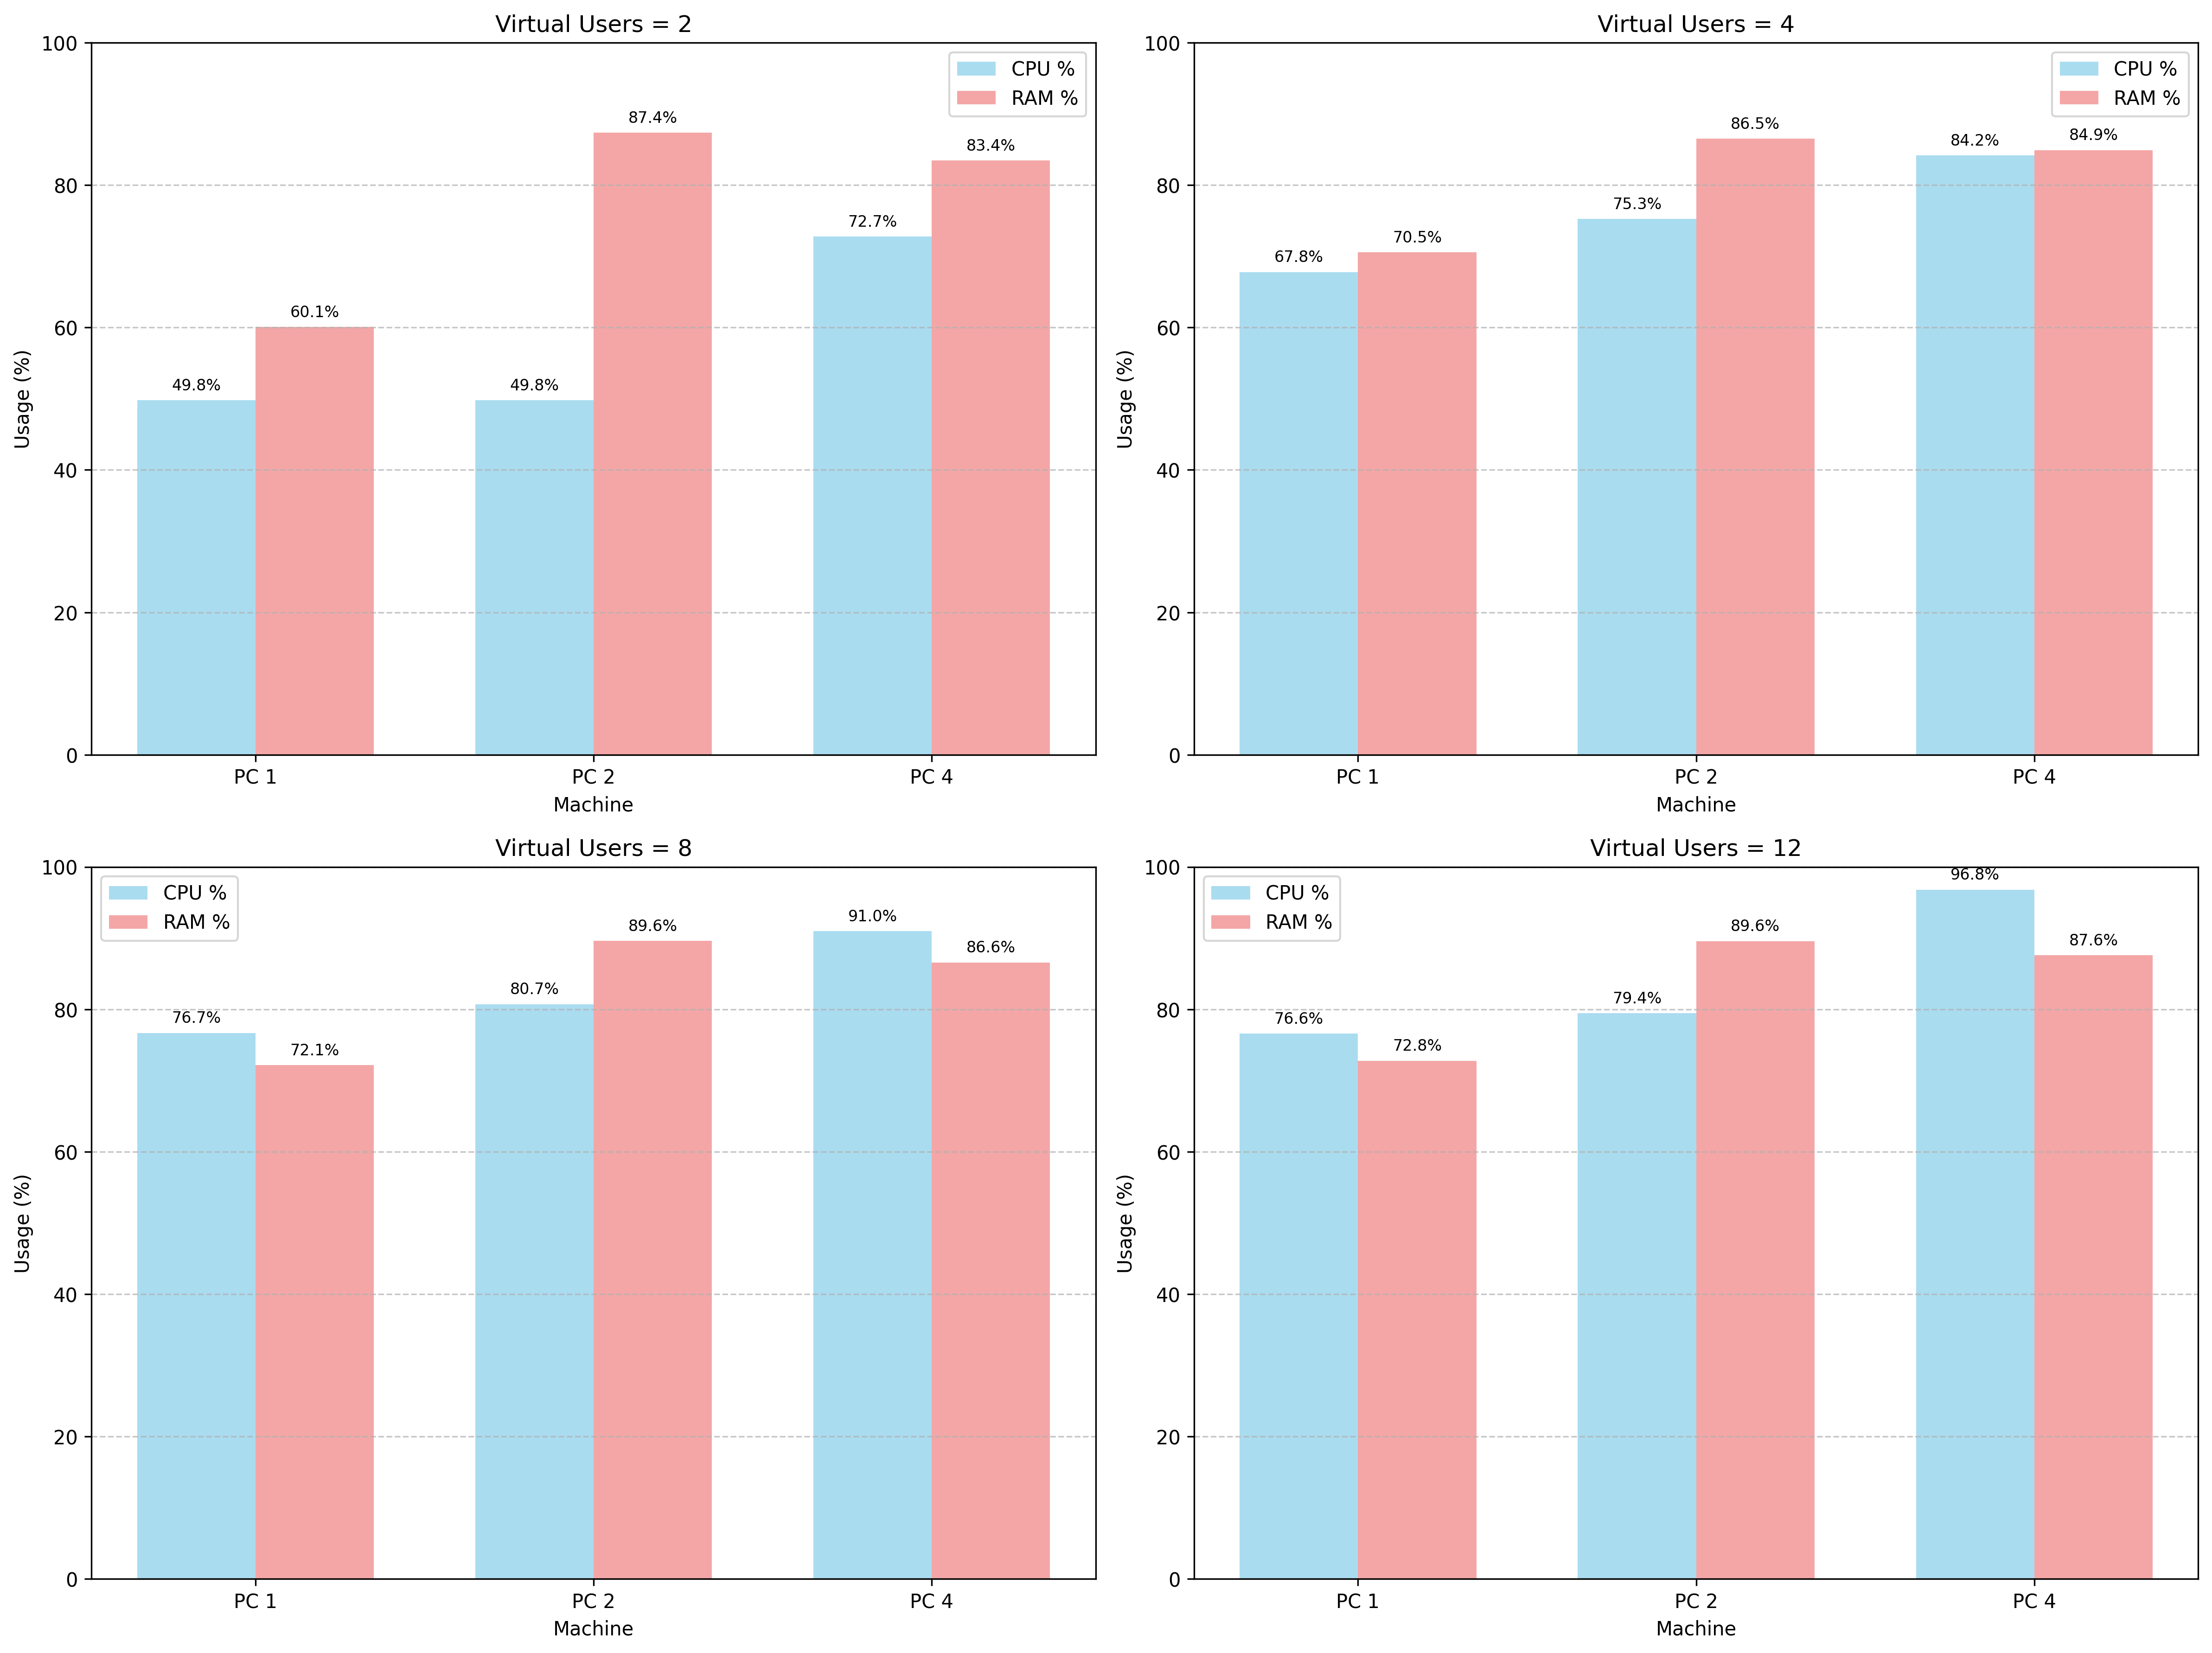
\includegraphics[width=0.87\linewidth]{Images/sys_usage_mysql_time_ranges_filtered.png}
    \caption{CPU and RAM usage on all tests using MySQL}
    \label{fig:mysql-cpu-ram}
\end{figure}

    \vspace{0.5cm}

\begin{figure}[H]
    \centering
    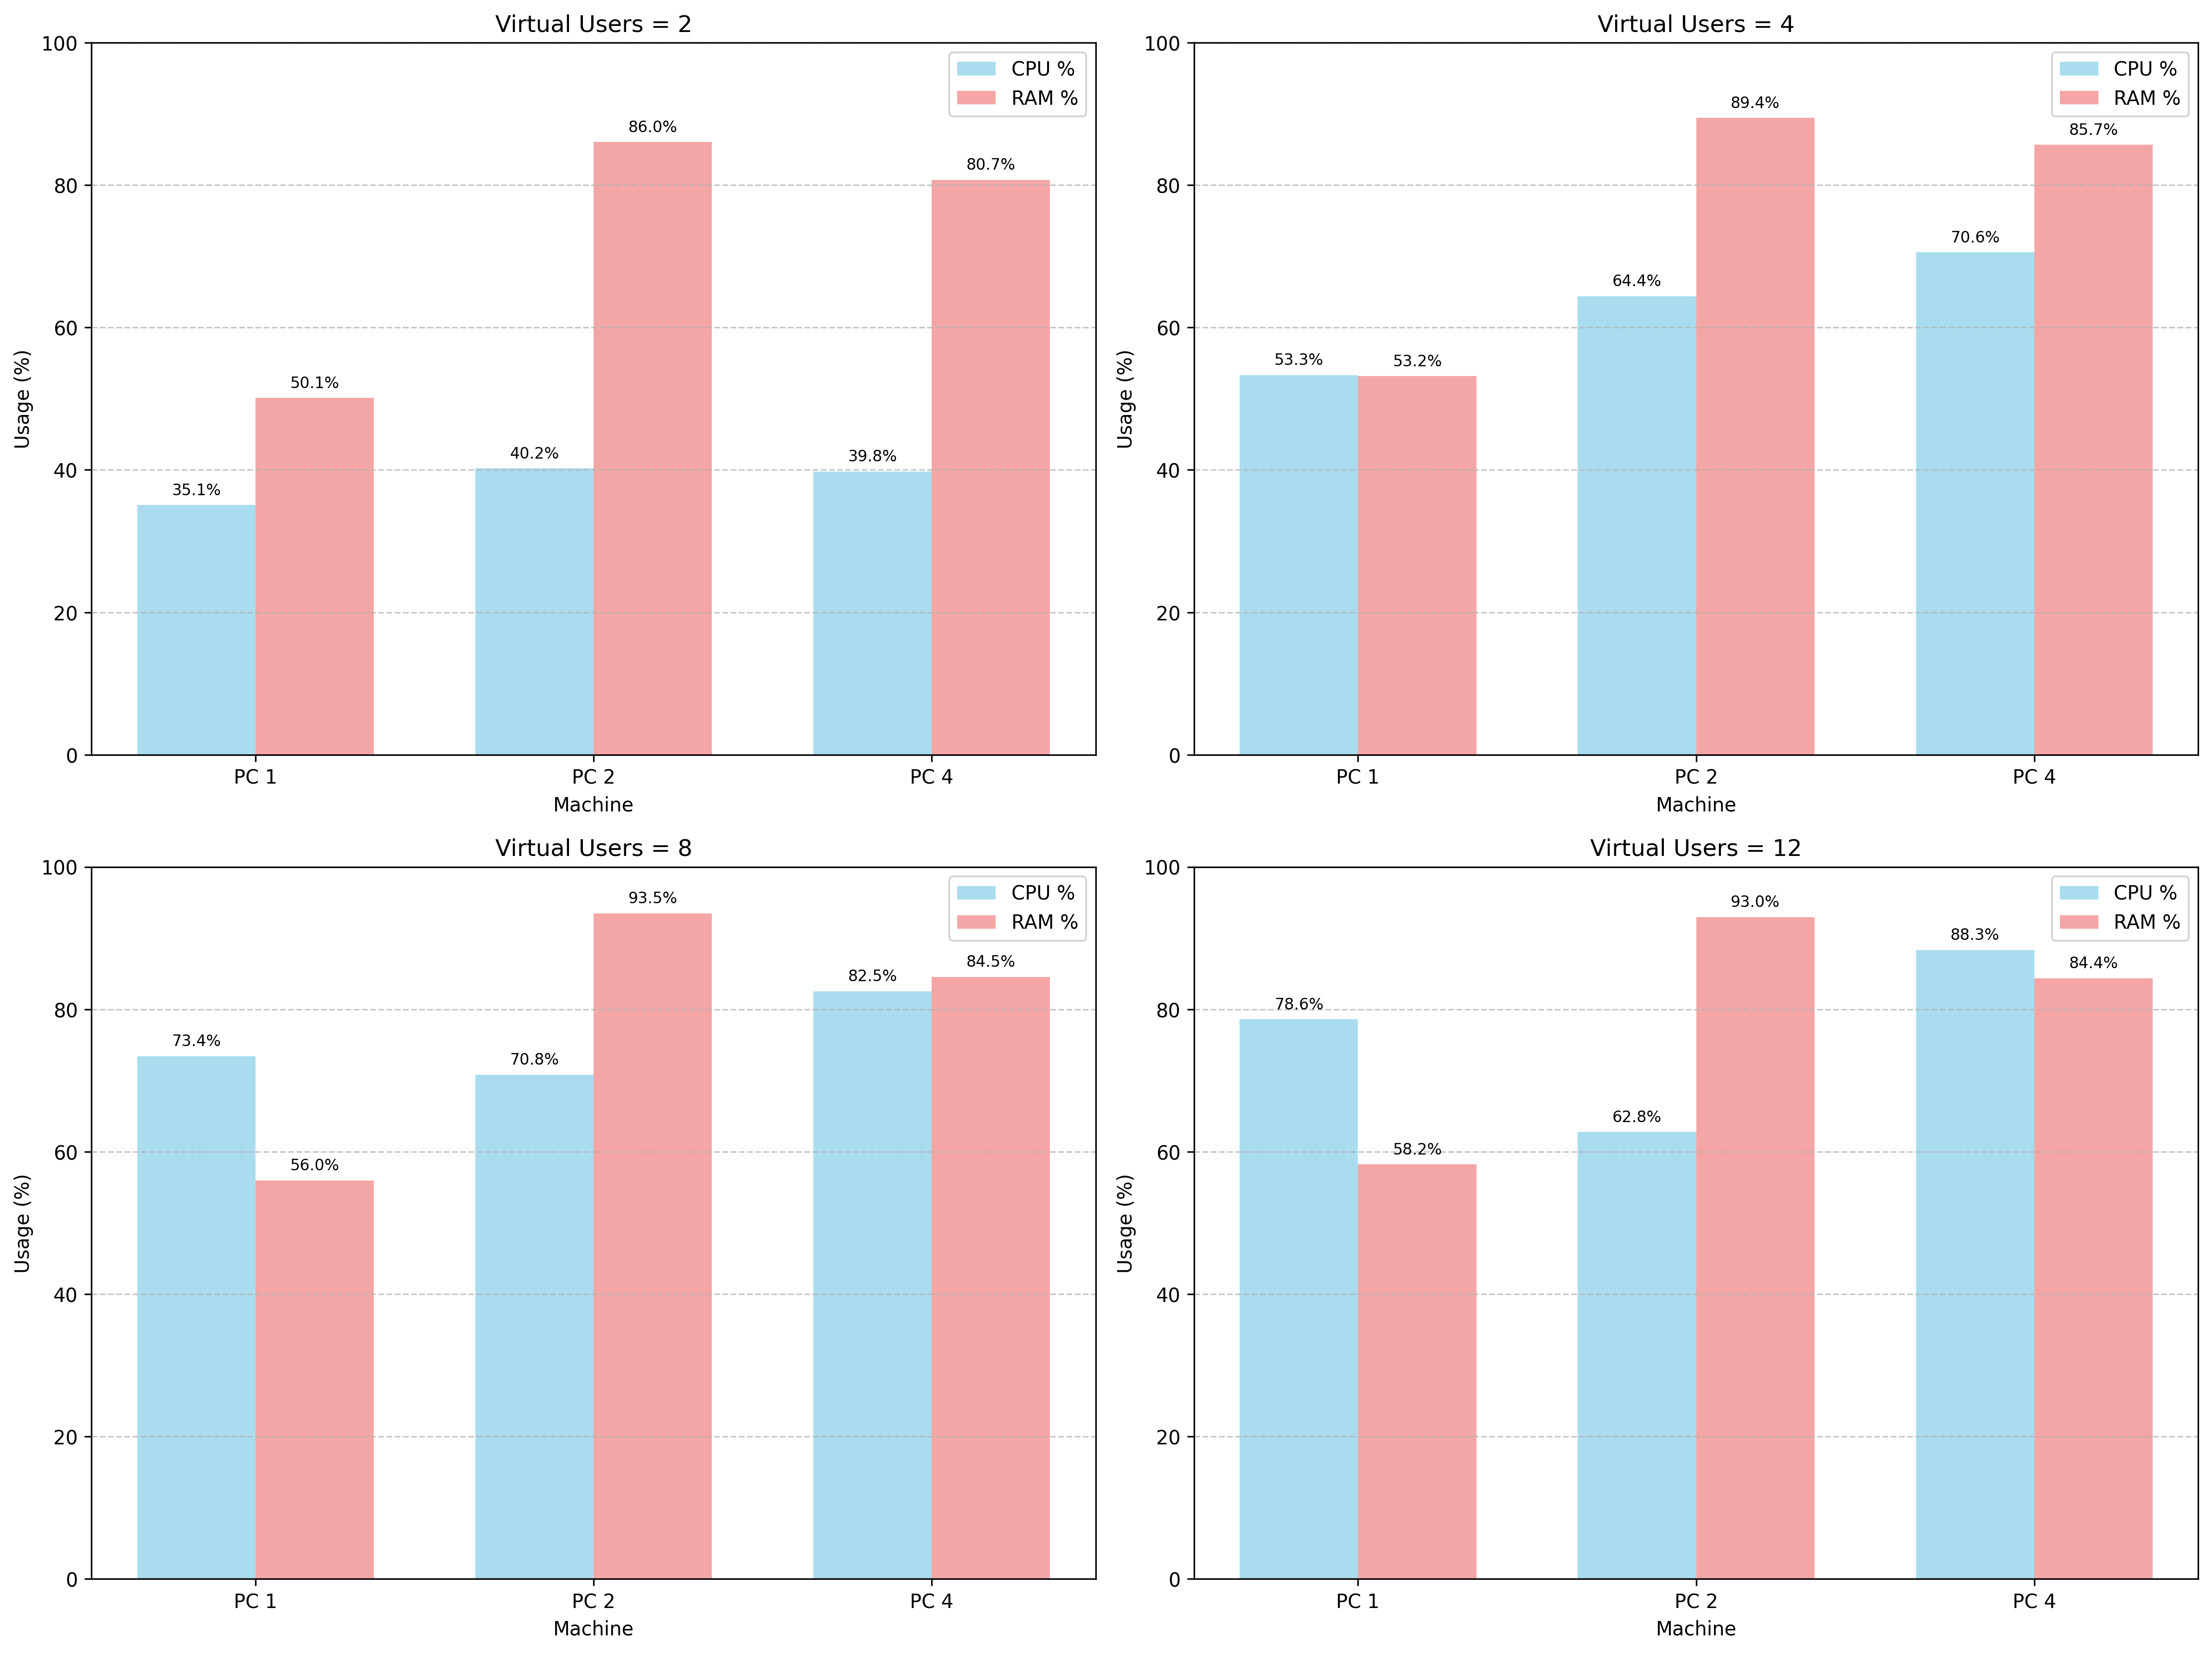
\includegraphics[width=0.87\linewidth]{Images/sys_usage_postgresql_time_ranges_filtered.png}
    \caption{CPU and RAM usage on all tests using PostgreSQL}
    \label{fig:pg-cpu-ram}    
\end{figure}

To ensure that there were no unexpected system bottlenecks that affected the benchmark results, we monitored both CPU and RAM usage during the tests with custom \hyperref[sec:pcstats-script]{scripts}. Disk usage was not recorded, as it is consistently at 100\% on all machines and is the main bottleneck in this type of workload.\\

In general, \textbf{\hyperref[tab:hardware-setup]{PC 1}} exhibited lower CPU and RAM usage compared to the others. This was expected as the slower disk likely acted as the limiting factor, preventing the CPU and memory from being fully utilized.\\

When comparing \textbf{\hyperref[tab:hardware-setup]{PC 2}} and \textbf{\hyperref[tab:hardware-setup]{PC 4}}, the first showed lower CPU usage. This can be attributed to its higher core count, an Intel processor with 14 cores (6 performance cores and 8 efficiency cores), compared to the Apple Silicon chip with only 8 cores (4 performance and 4 efficiency cores). On the other hand, PC 4 demonstrated lower RAM usage, which is likely due to the more efficient memory management capabilities of macOS.

\subsection{Use All Warehouses Comparison}

\begin{figure}[H]
    \centering
    \hspace*{-1.7cm}
    \begin{subfigure}[b]{0.6\textwidth}
        \centering
        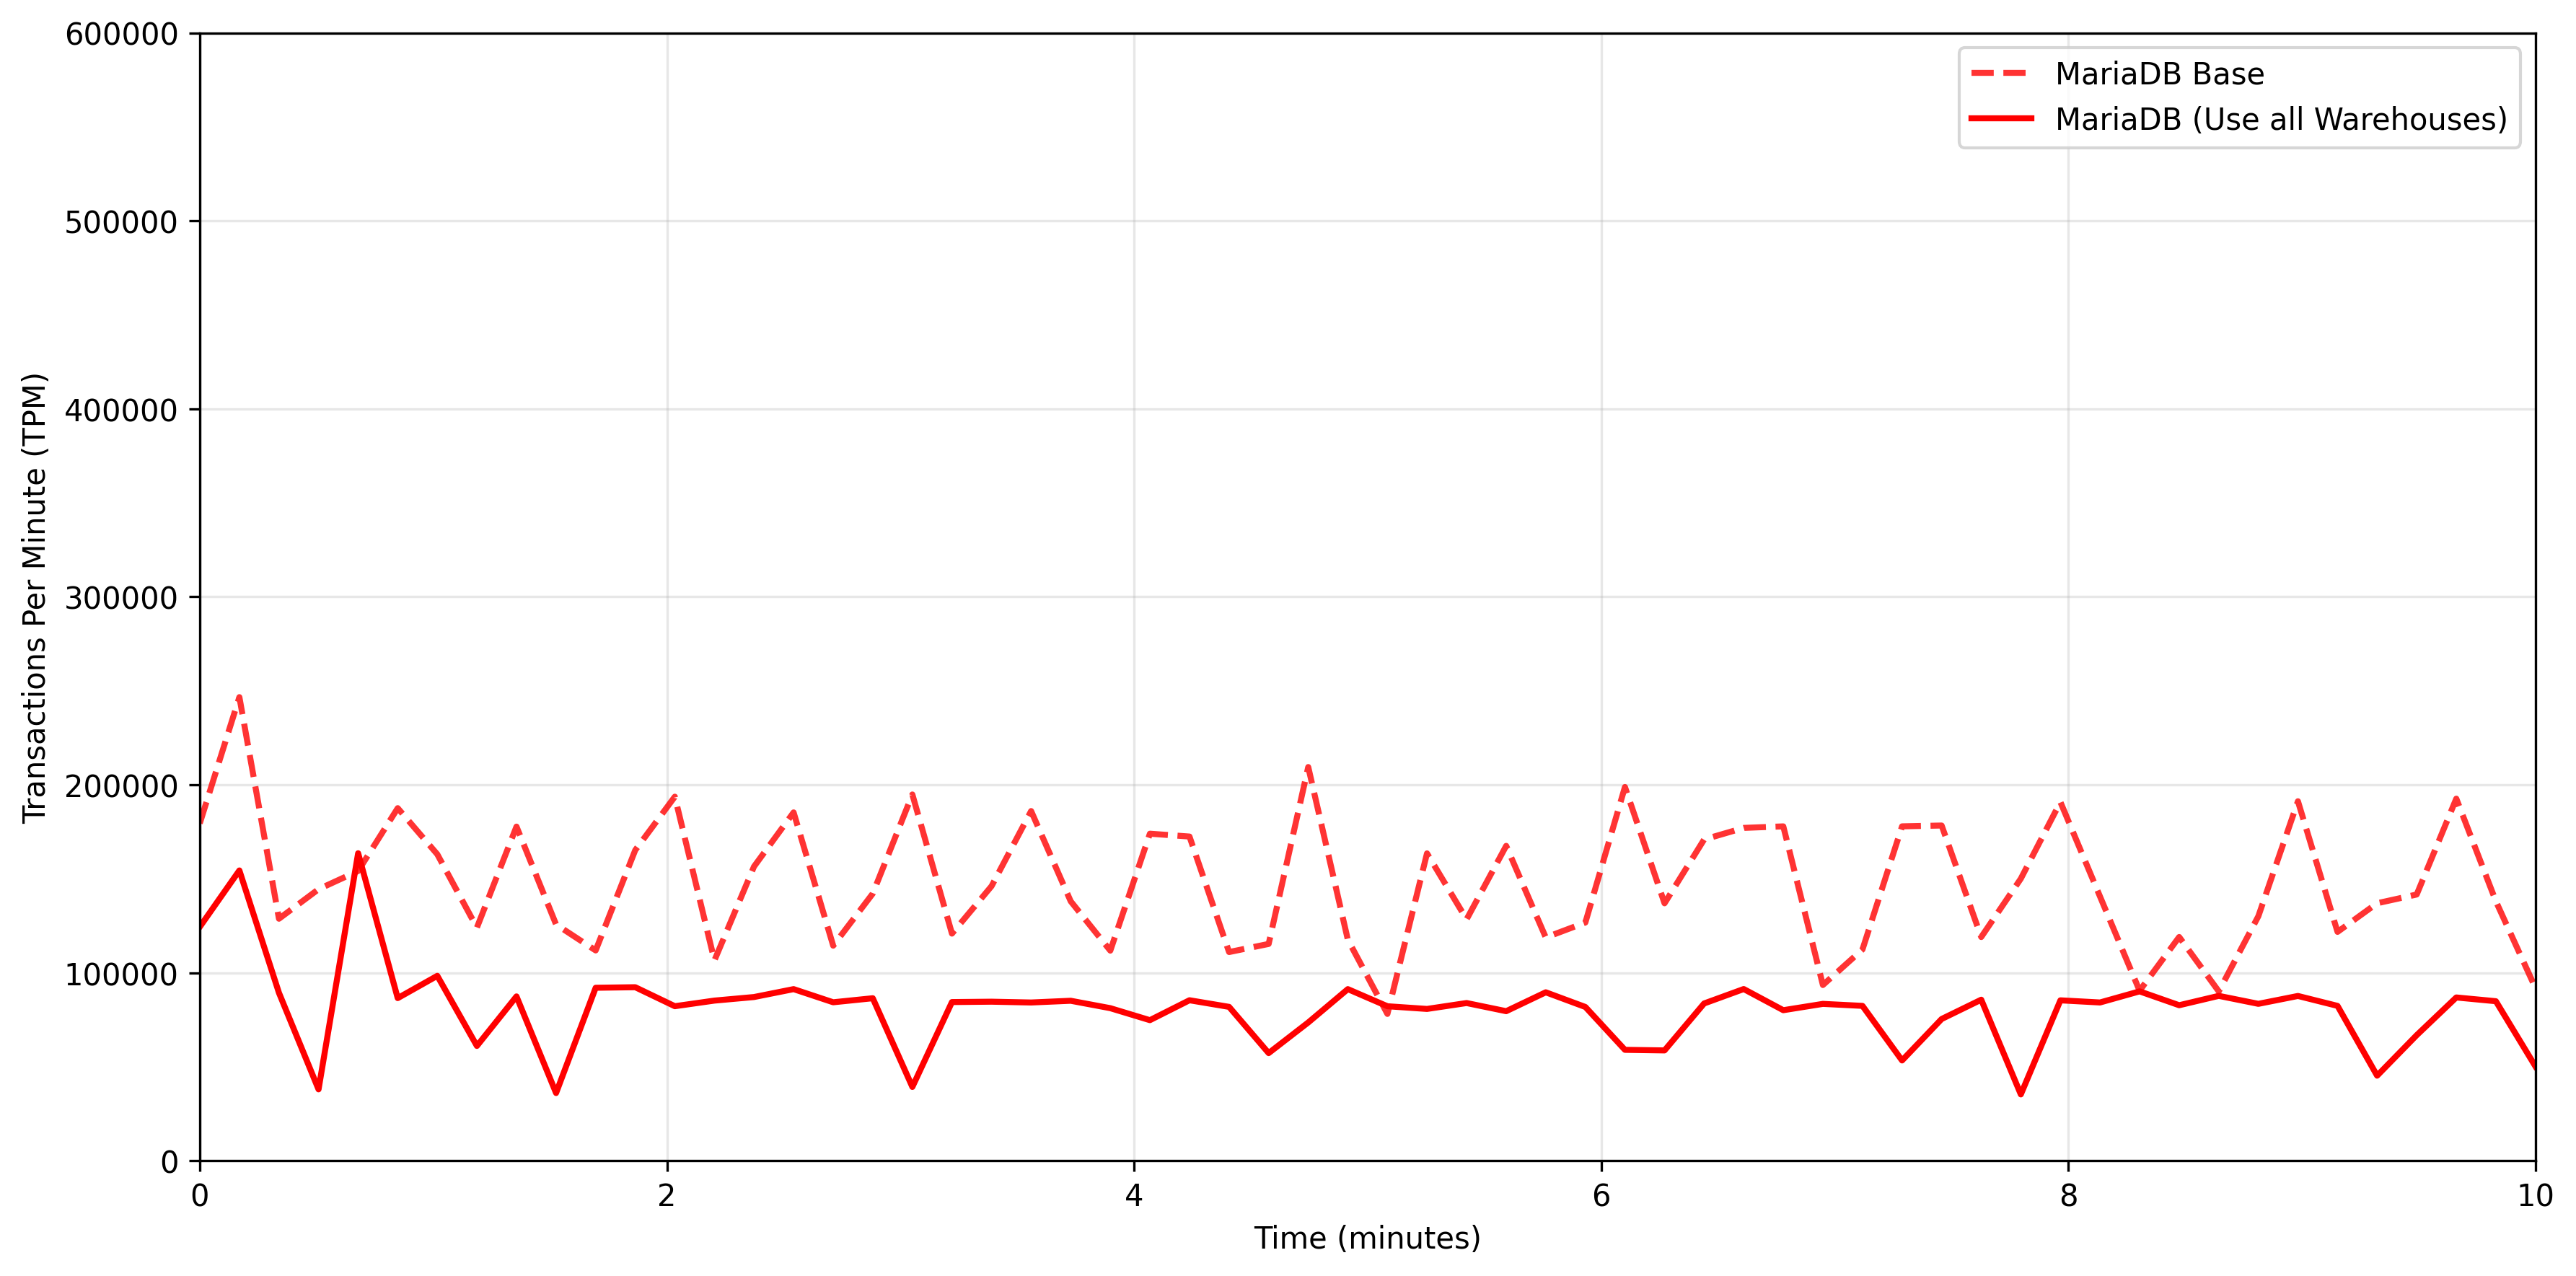
\includegraphics[width=\linewidth]{Images/database_count_comparison_MariaDB.png}
        \caption{Comparison in MariaDB}
        \label{fig:all-wh-maria}
    \end{subfigure}%
    \begin{subfigure}[b]{0.6\textwidth}
        \centering
        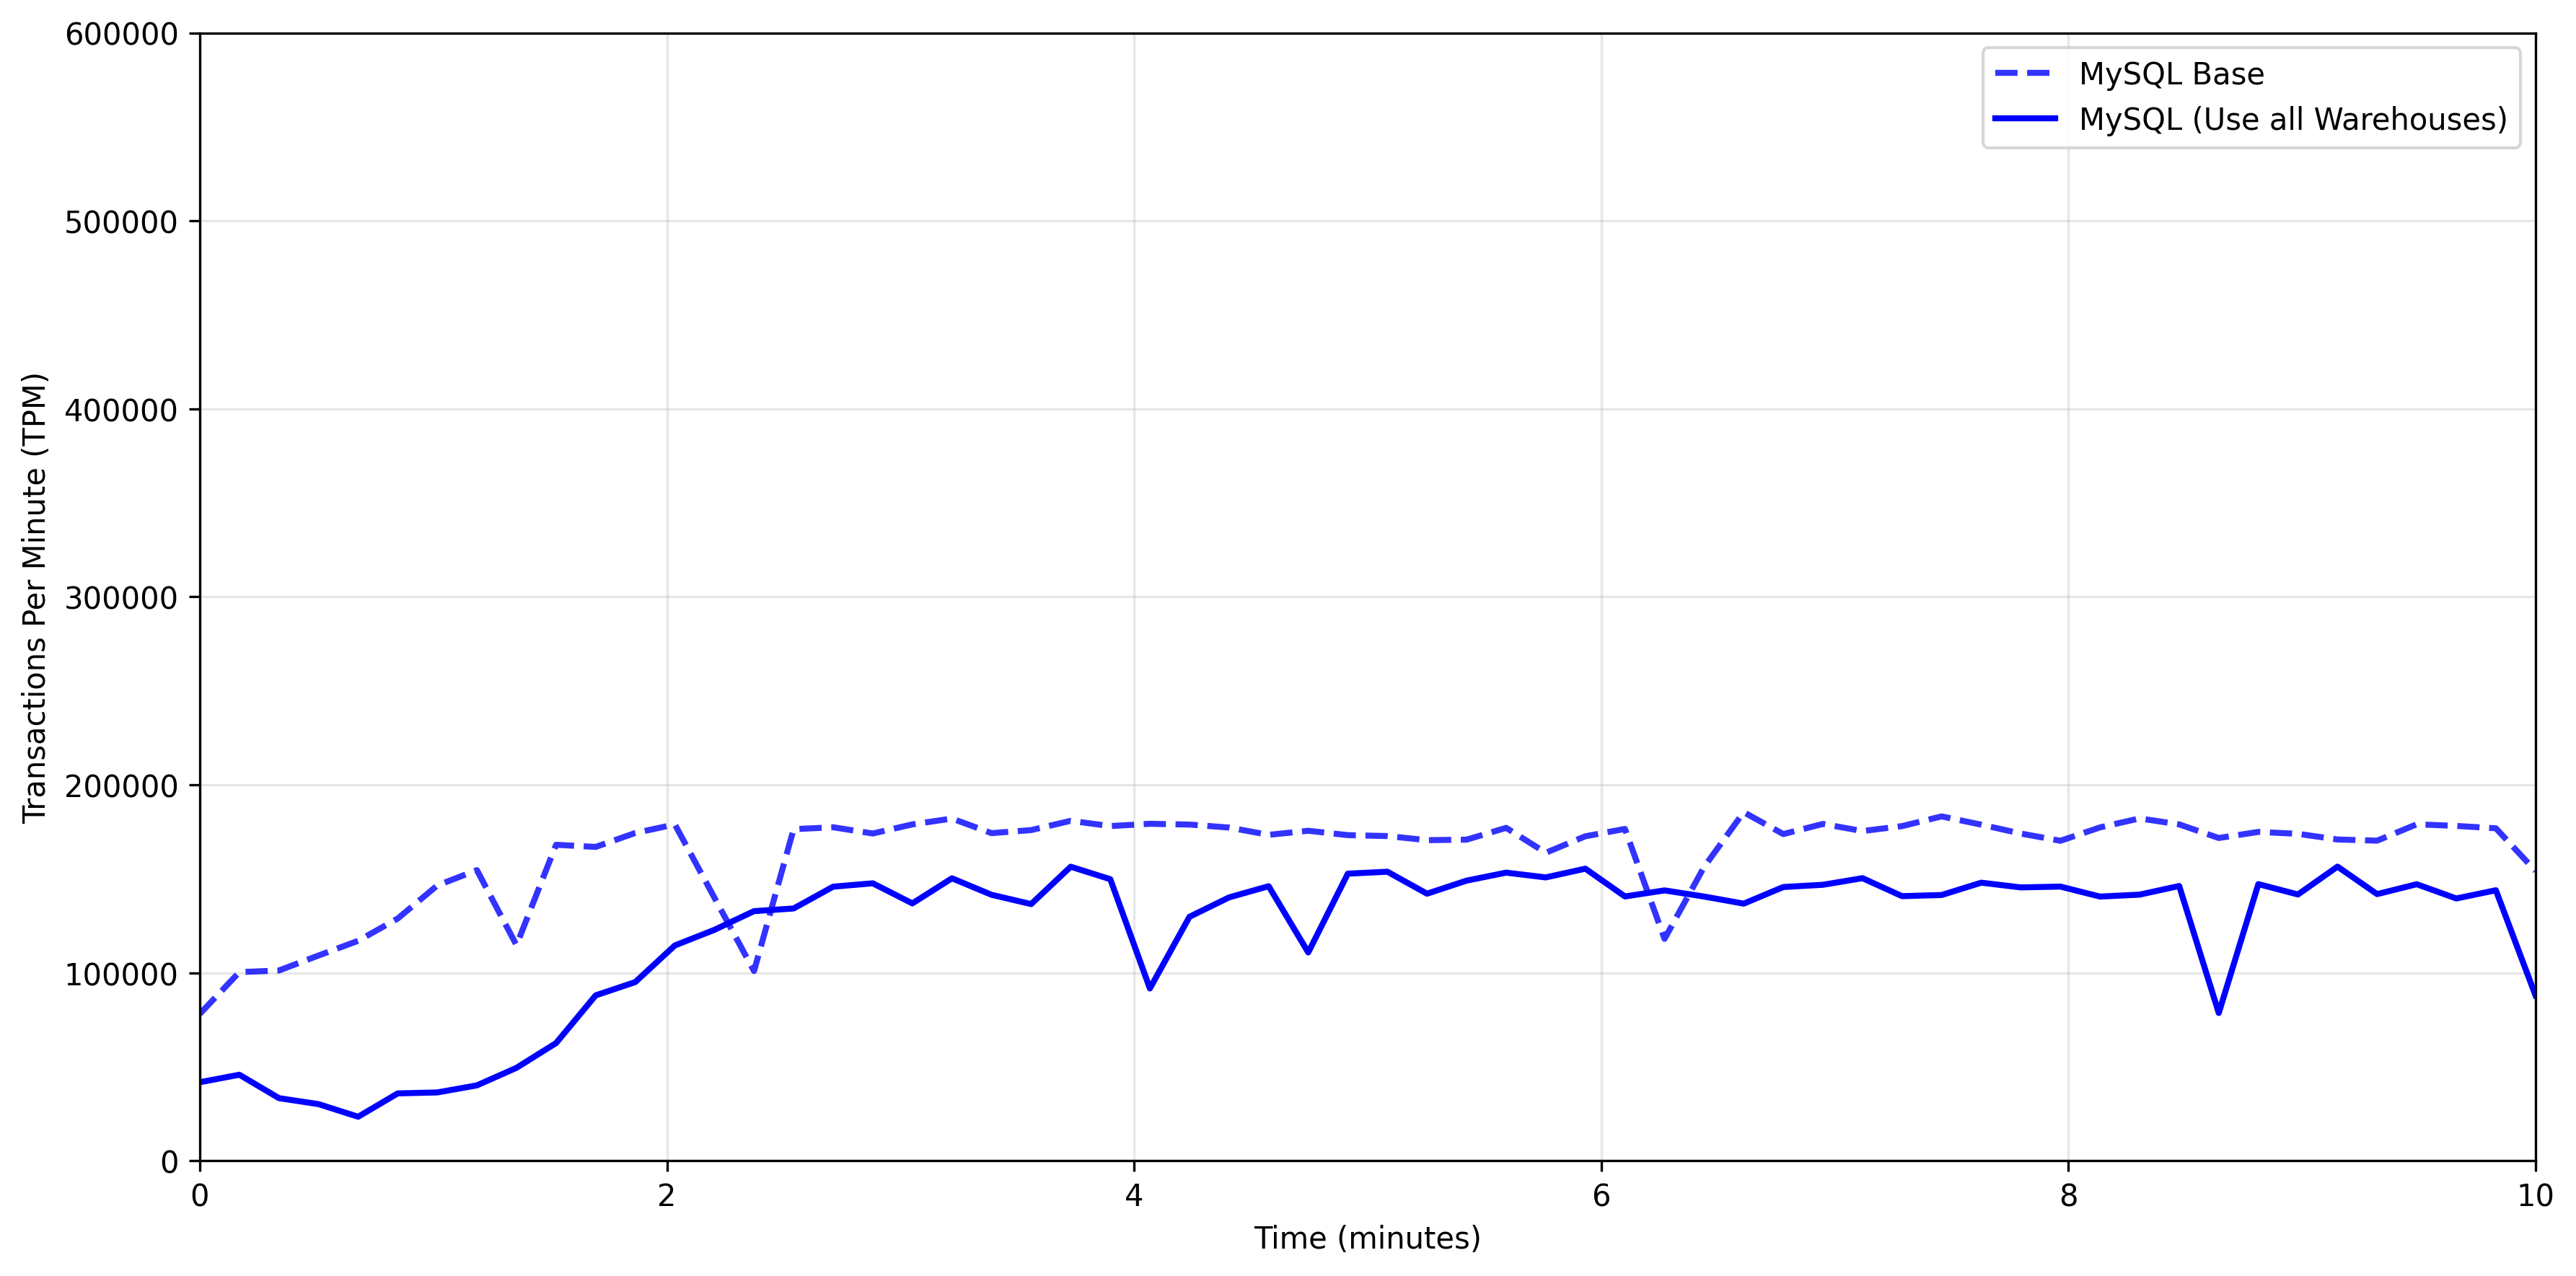
\includegraphics[width=\linewidth]{Images/database_count_comparison_MySQL.png}
        \caption{Comparison in MySQL}
        \label{fig:all-wh-mysql}
    \end{subfigure}

    \vspace{0.5cm}

    \hspace*{-1.7cm}
    \begin{subfigure}[b]{0.6\textwidth}
        \centering
        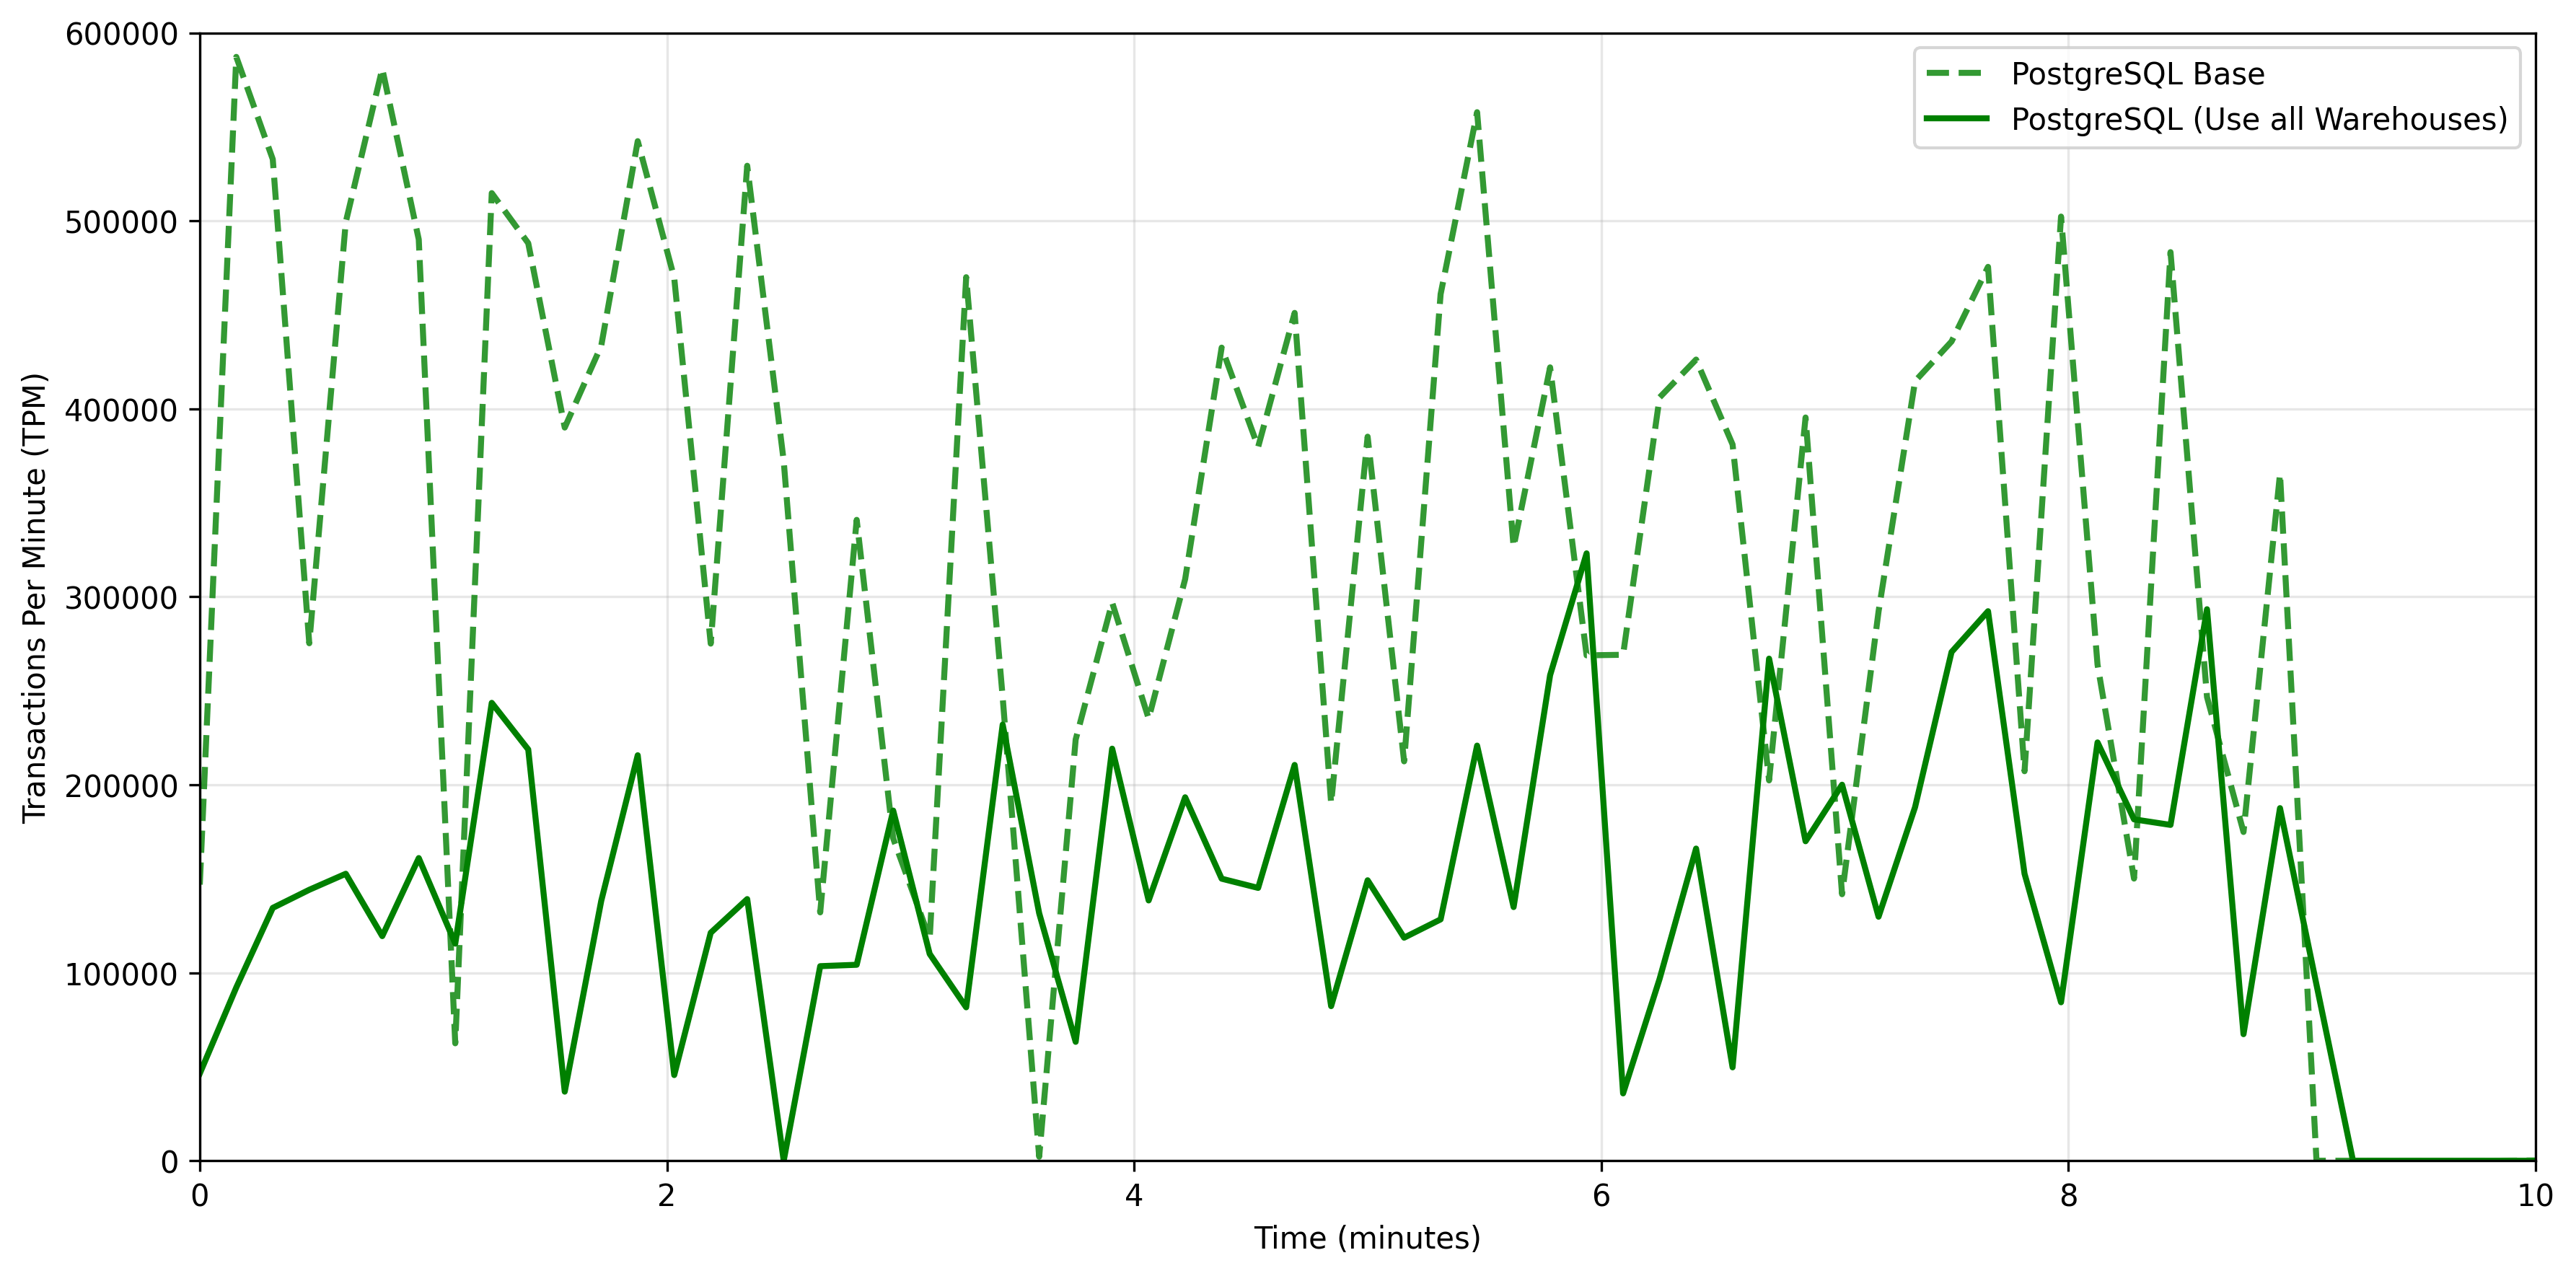
\includegraphics[width=\linewidth]{Images/database_count_comparison_PostgreSQL.png}
        \caption{Comparison in PostgreSQL}
        \label{fig:all-wh-pg}
    \end{subfigure}%
    \begin{subfigure}[b]{0.6\textwidth}
        \centering
        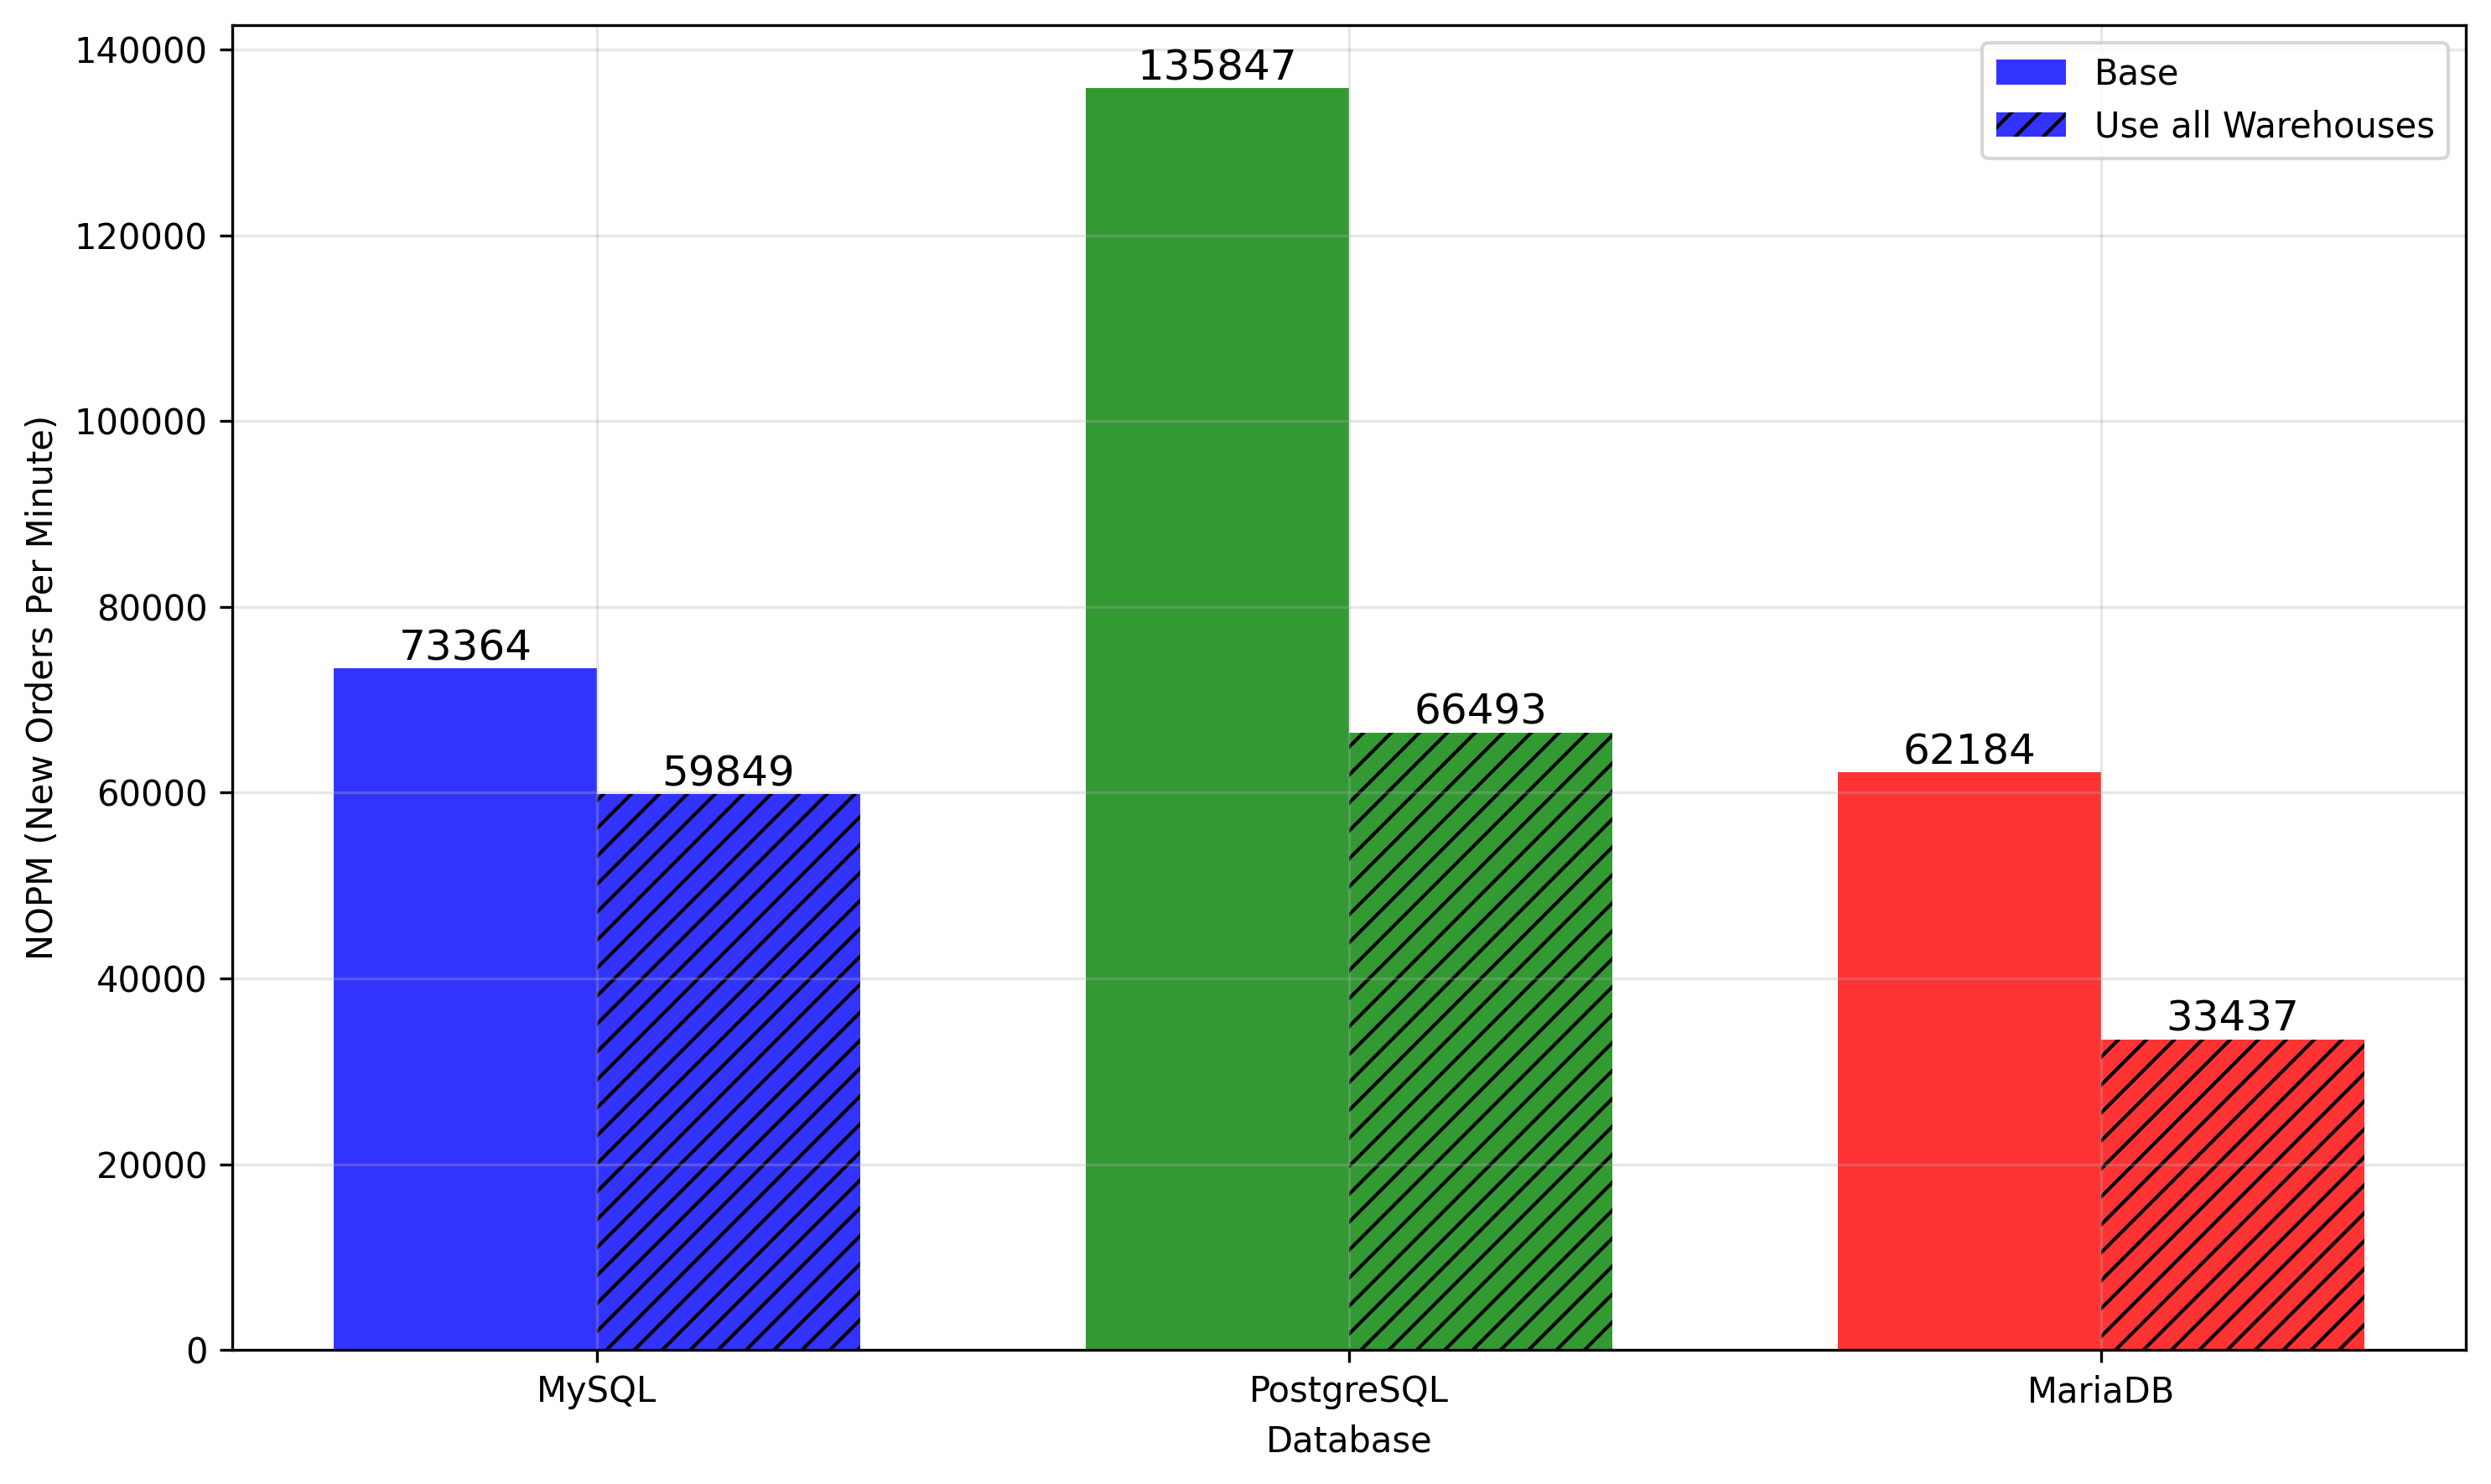
\includegraphics[width=\linewidth]{Images/hammerdb_summary_comparison_vu12.png}
        \caption{NOPM results for all Databases}
        \label{fig:all-wh-summary}
    \end{subfigure}

    \caption{'Use All Warehouses' performance analysis for VU=12 and WH=60 on PC 1}
    \label{fig:all-wh}
\end{figure}

One of the configurable test parameters is the "Use All Warehouses" option, which simulates a more realistic multi-user environment by allowing clients to access different data partitions concurrently. This setup provides a better assessment of how well a database handles distributed load and concurrent access. However, it also introduces increased randomness in data access, reduces cache effectiveness, and places additional pressure on the disk subsystem. To better observe the impact of this option, the test was run on \textbf{\hyperref[tab:hardware-setup]{PC 1}}, which has the slowest disk among all machines.\\

As expected, the average TPM dropped across all database configurations when the "Use All Warehouses" option was enabled, likely due to increased disk I/O demands. Interestingly, MySQL handled the change relatively well, with only an 18.4\% drop in NOPM performance. In contrast, PostgreSQL and MariaDB experienced much steeper declines, losing 51.1\% and 46.27\% of their NOPM performance, respectively. This outcome was somewhat surprising, as PostgreSQL is known for its robust concurrency features. As for the differences between MySQL and MariaDB, they could be attributed to several factors, such as concurrency improvements in newer versions of InnoDB that are present in MySQL but not in MariaDB, or additional overhead in MariaDB’s lock and thread management implementations, under high-concurrency and I/O-intensive workloads. \\

In summary, "Use All Warehouses" provides a more realistic and comprehensive performance scenario, which reveals potential I/O bottlenecks, especially on systems with limited storage throughput. It serves as a valuable stress test for high-concurrency environments.

\subsection{Final comparison between Databases}

\begin{figure}[H]
    \centering
    \hspace*{-1.7cm}
    \begin{subfigure}[b]{0.6\textwidth}
        \centering
        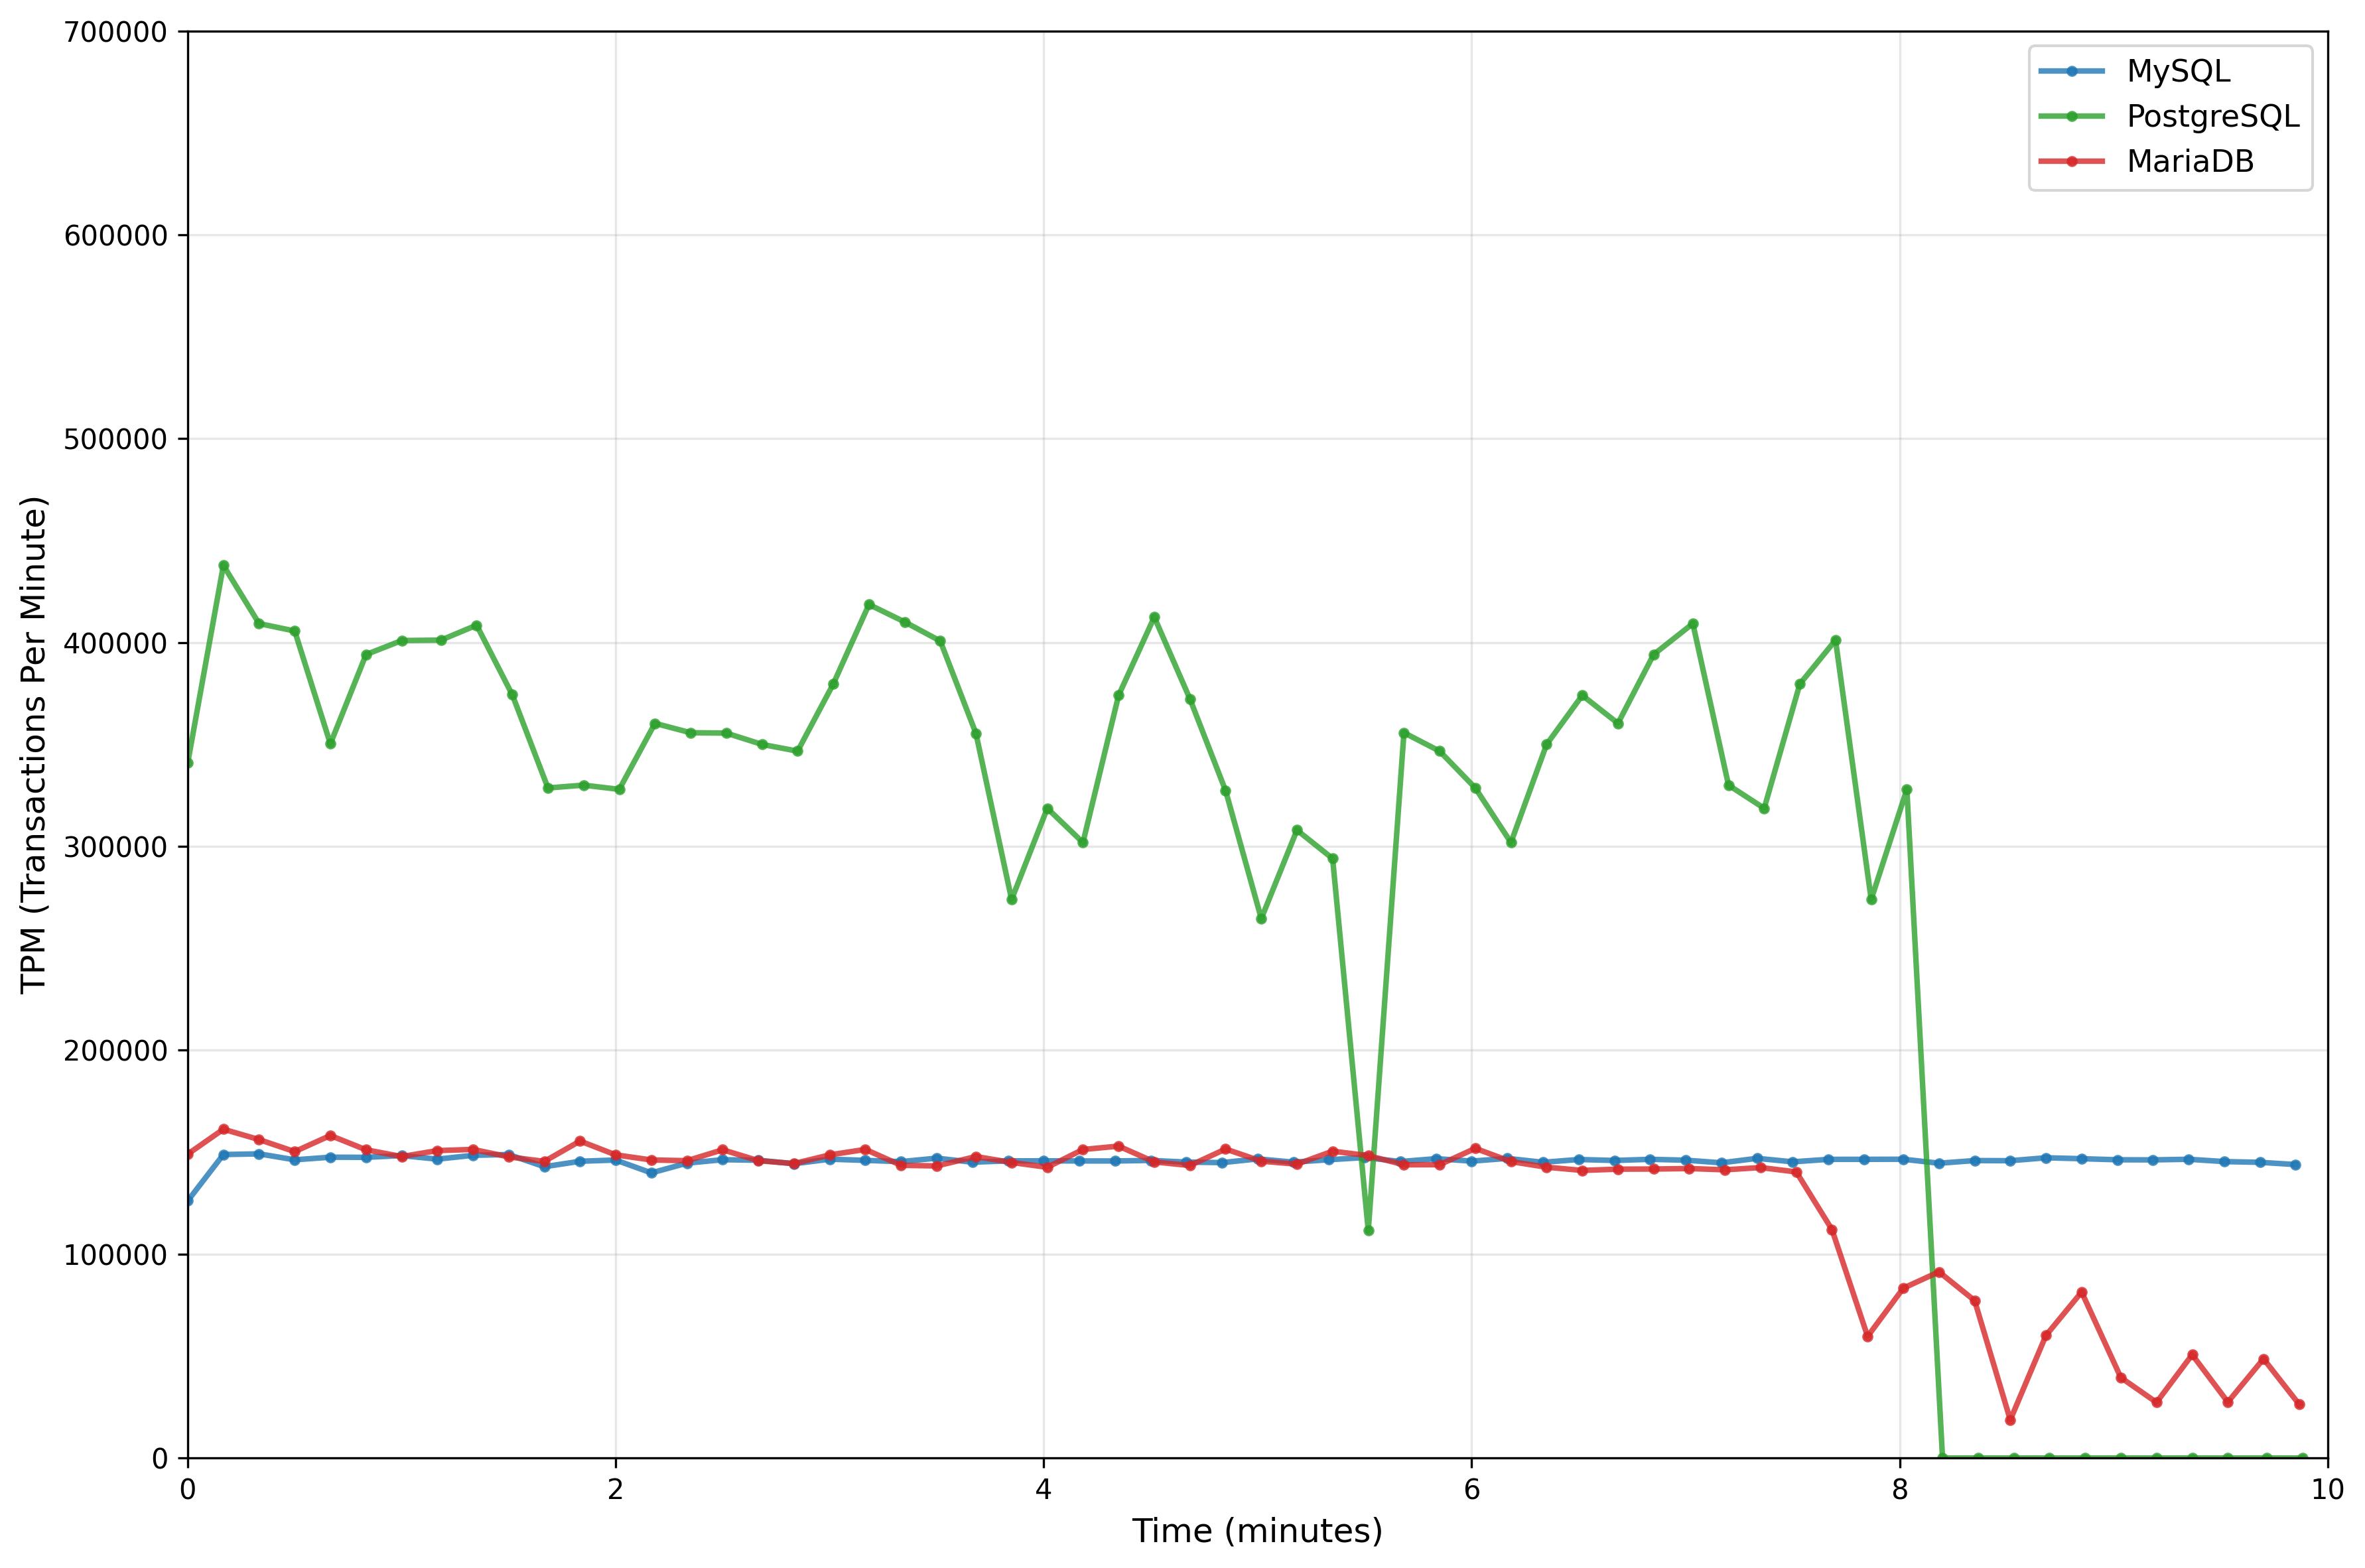
\includegraphics[width=\linewidth]{Images/db_comparison_2_users.png}
        \caption{Database results with 2 Virtual Users}
        \label{fig:db-2vu}
    \end{subfigure}%
    \begin{subfigure}[b]{0.6\textwidth}
        \centering
        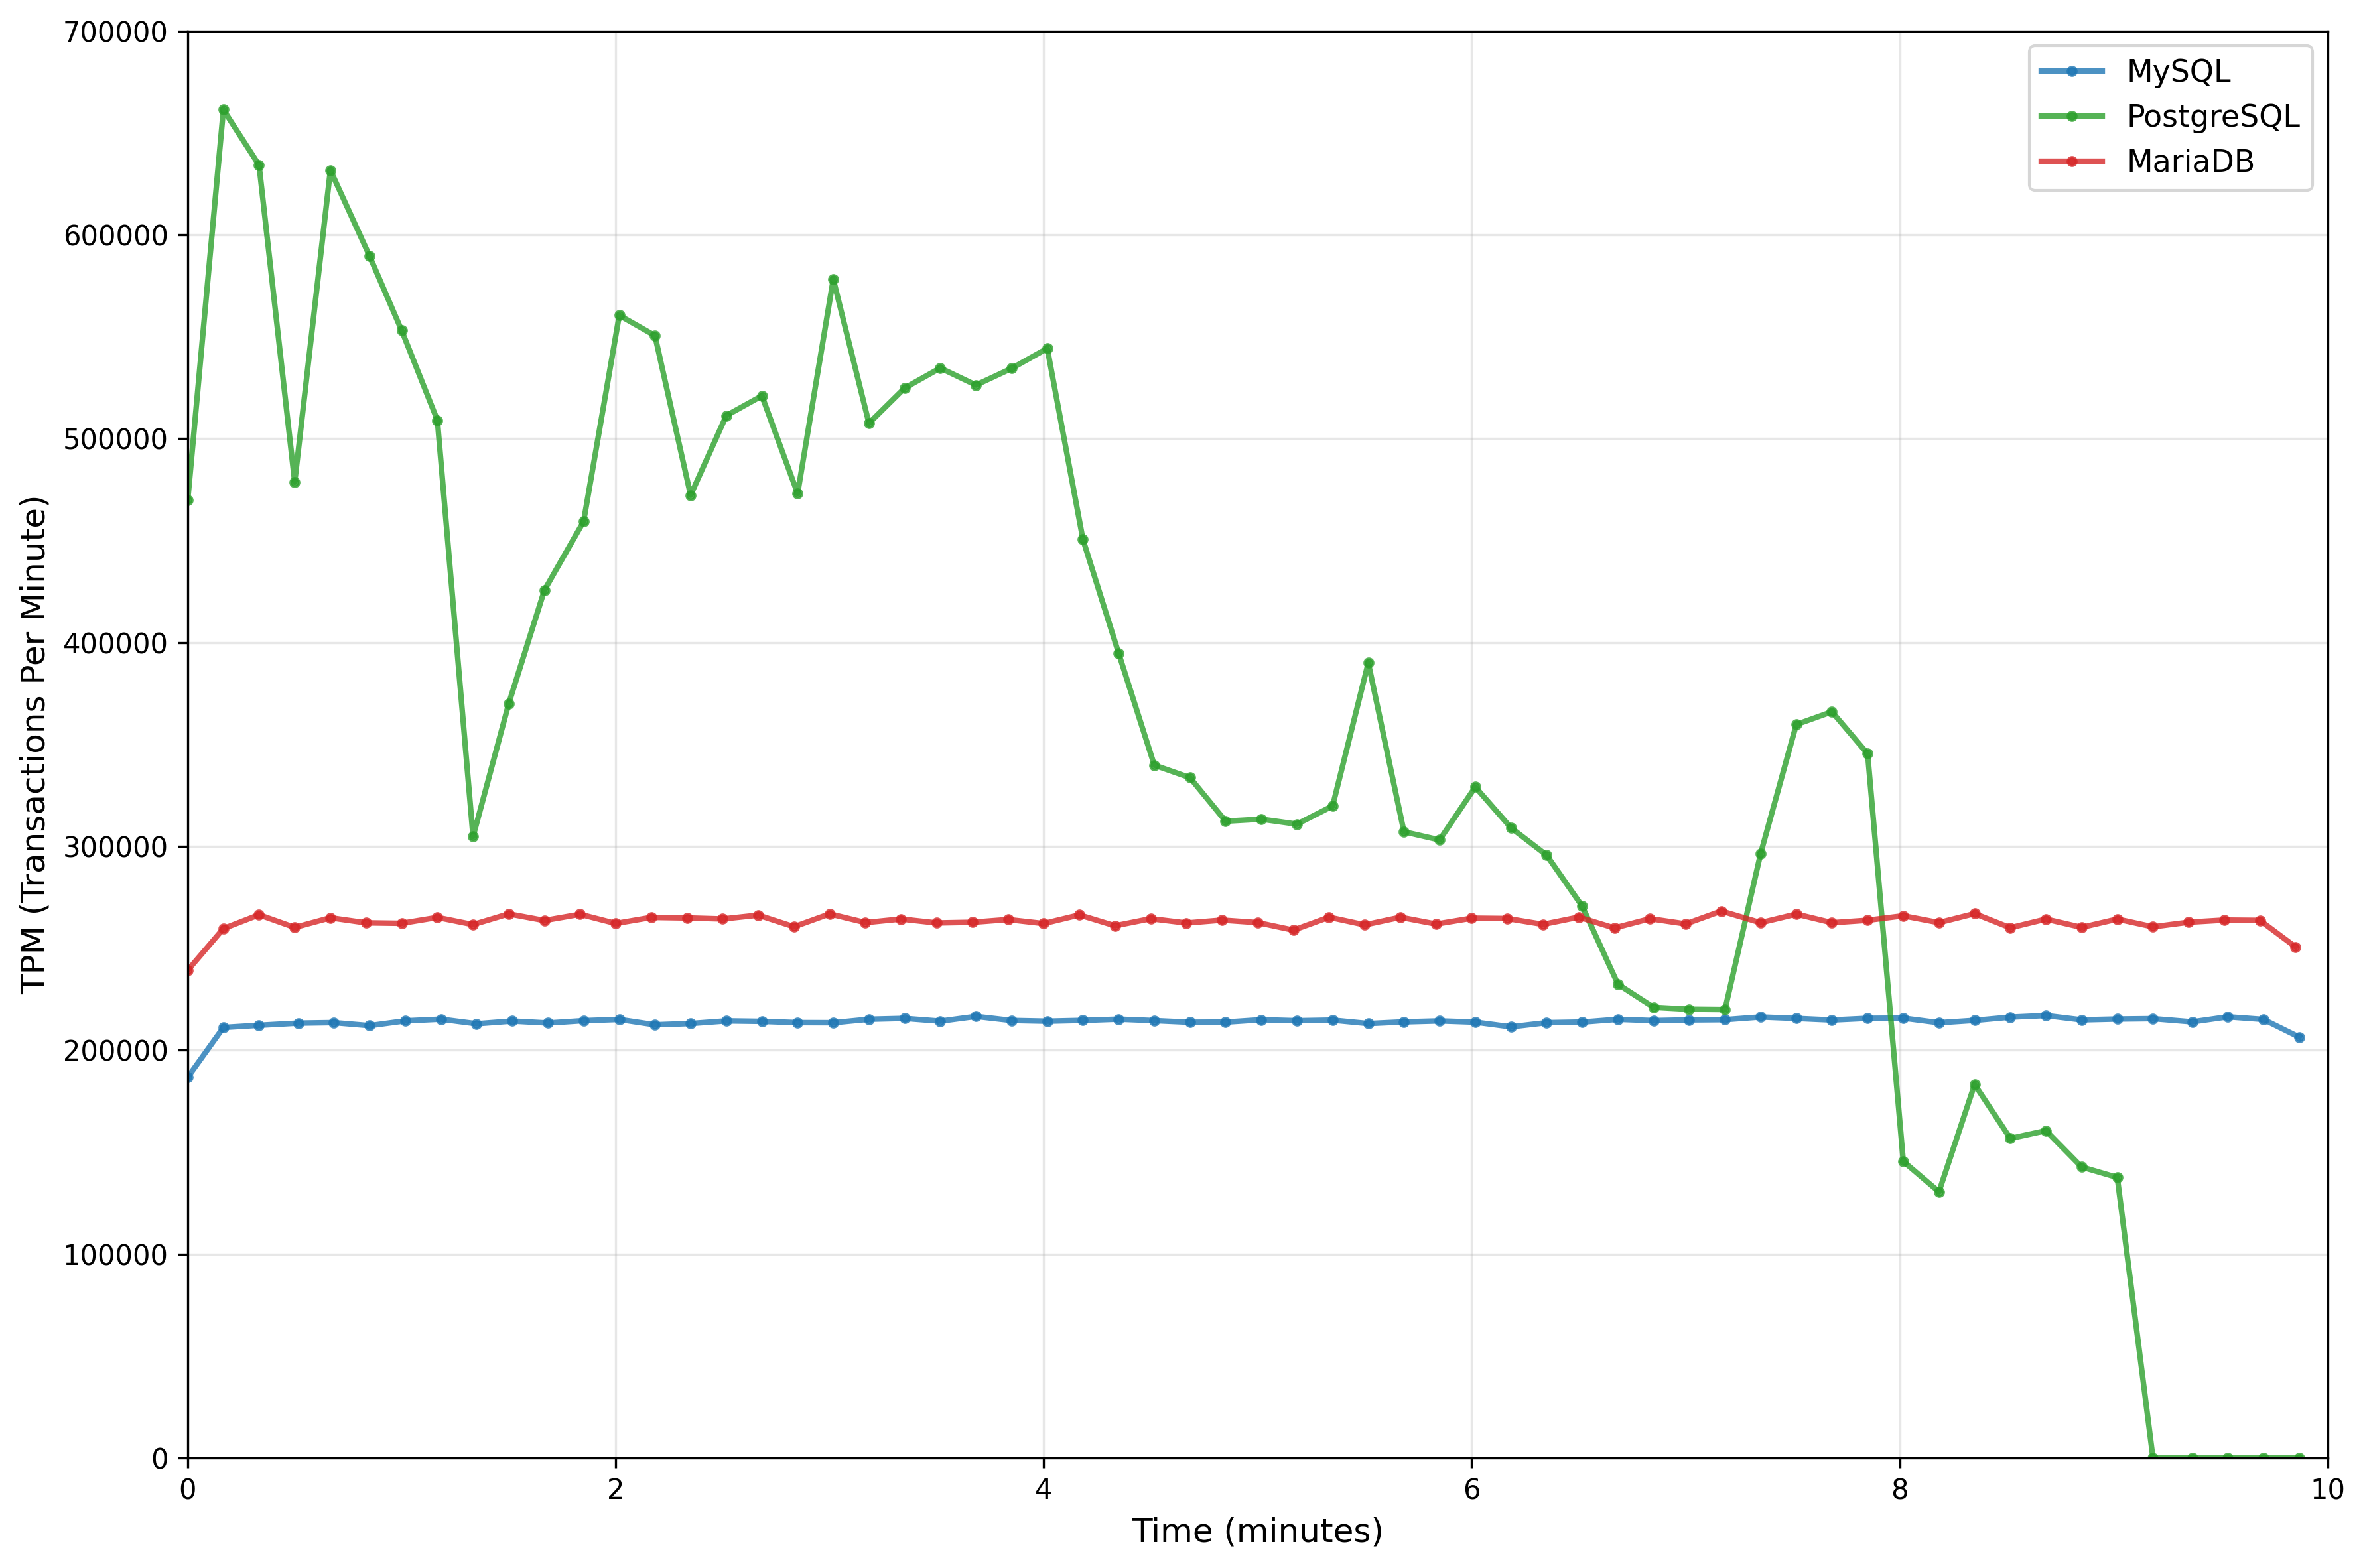
\includegraphics[width=\linewidth]{Images/db_comparison_4_users.png}
        \caption{Database results with 4 Virtual Users}
        \label{fig:db-4vu}
    \end{subfigure}

    \vspace{0.5cm}

    \hspace*{-1.7cm}
    \begin{subfigure}[b]{0.6\textwidth}
        \centering
        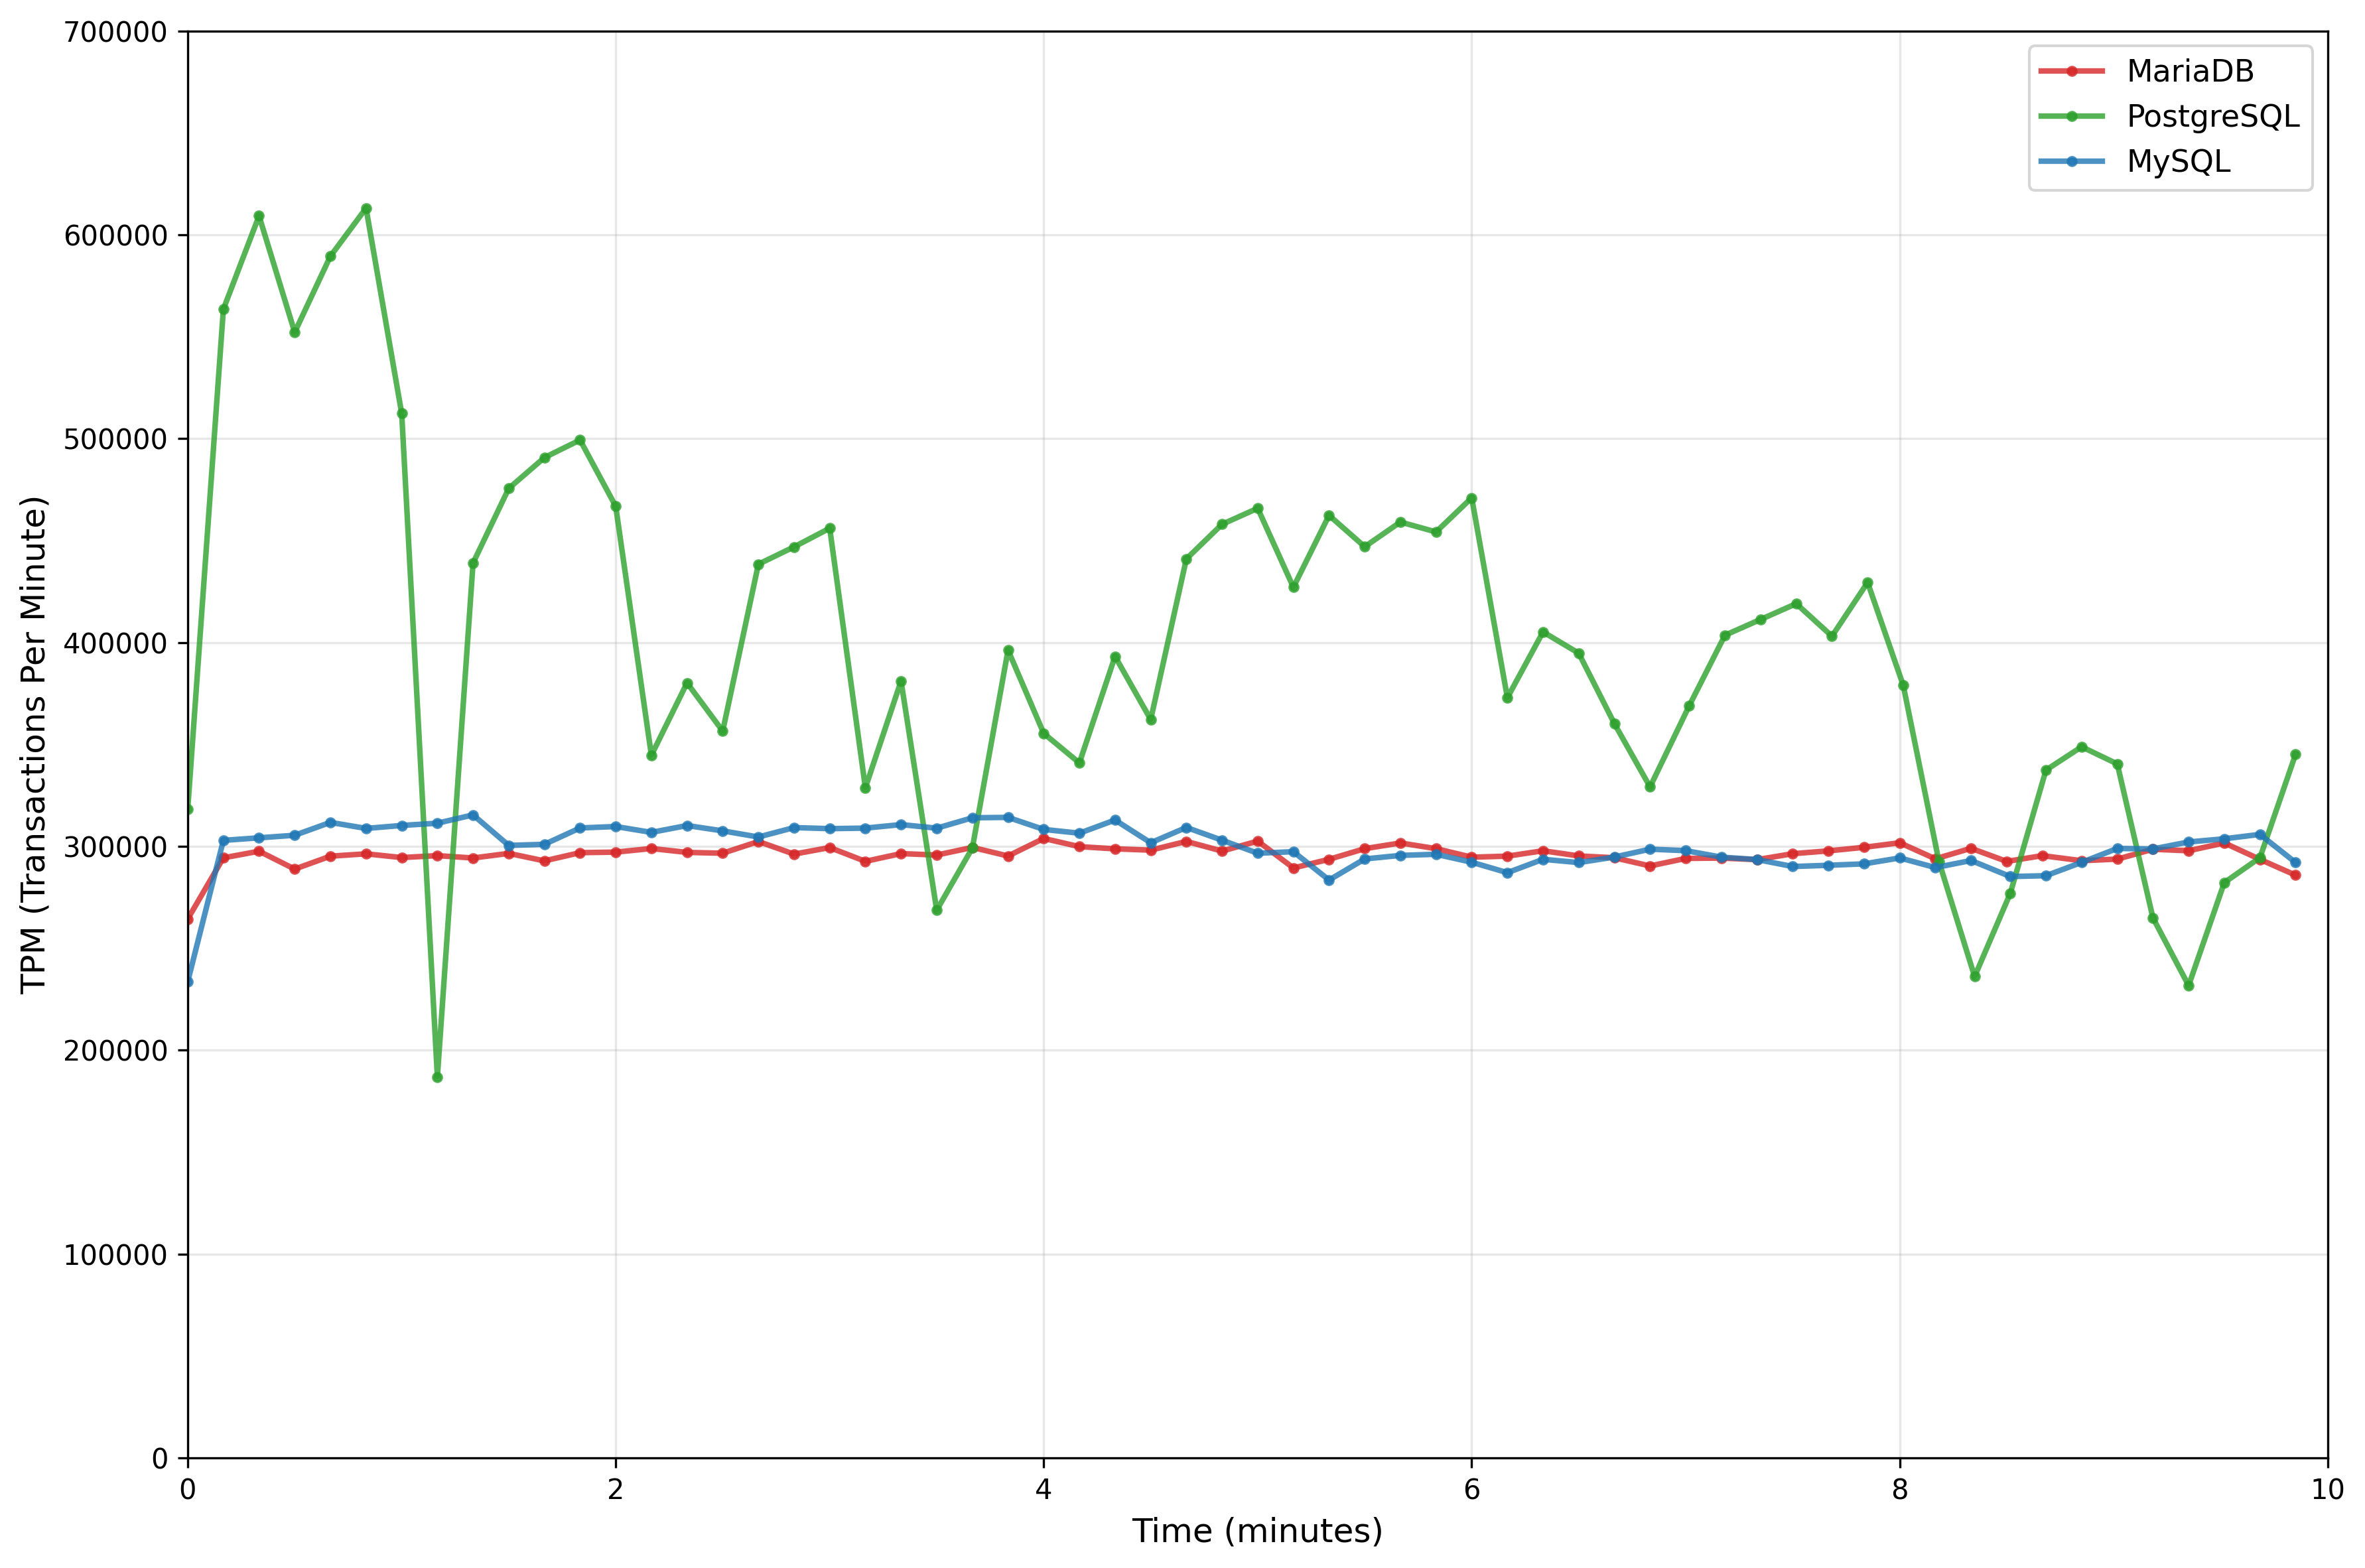
\includegraphics[width=\linewidth]{Images/db_comparison_8_users.png}
        \caption{Database results with 8 Virtual Users}
        \label{fig:db-8vu}
    \end{subfigure}%
    \begin{subfigure}[b]{0.6\textwidth}
        \centering
        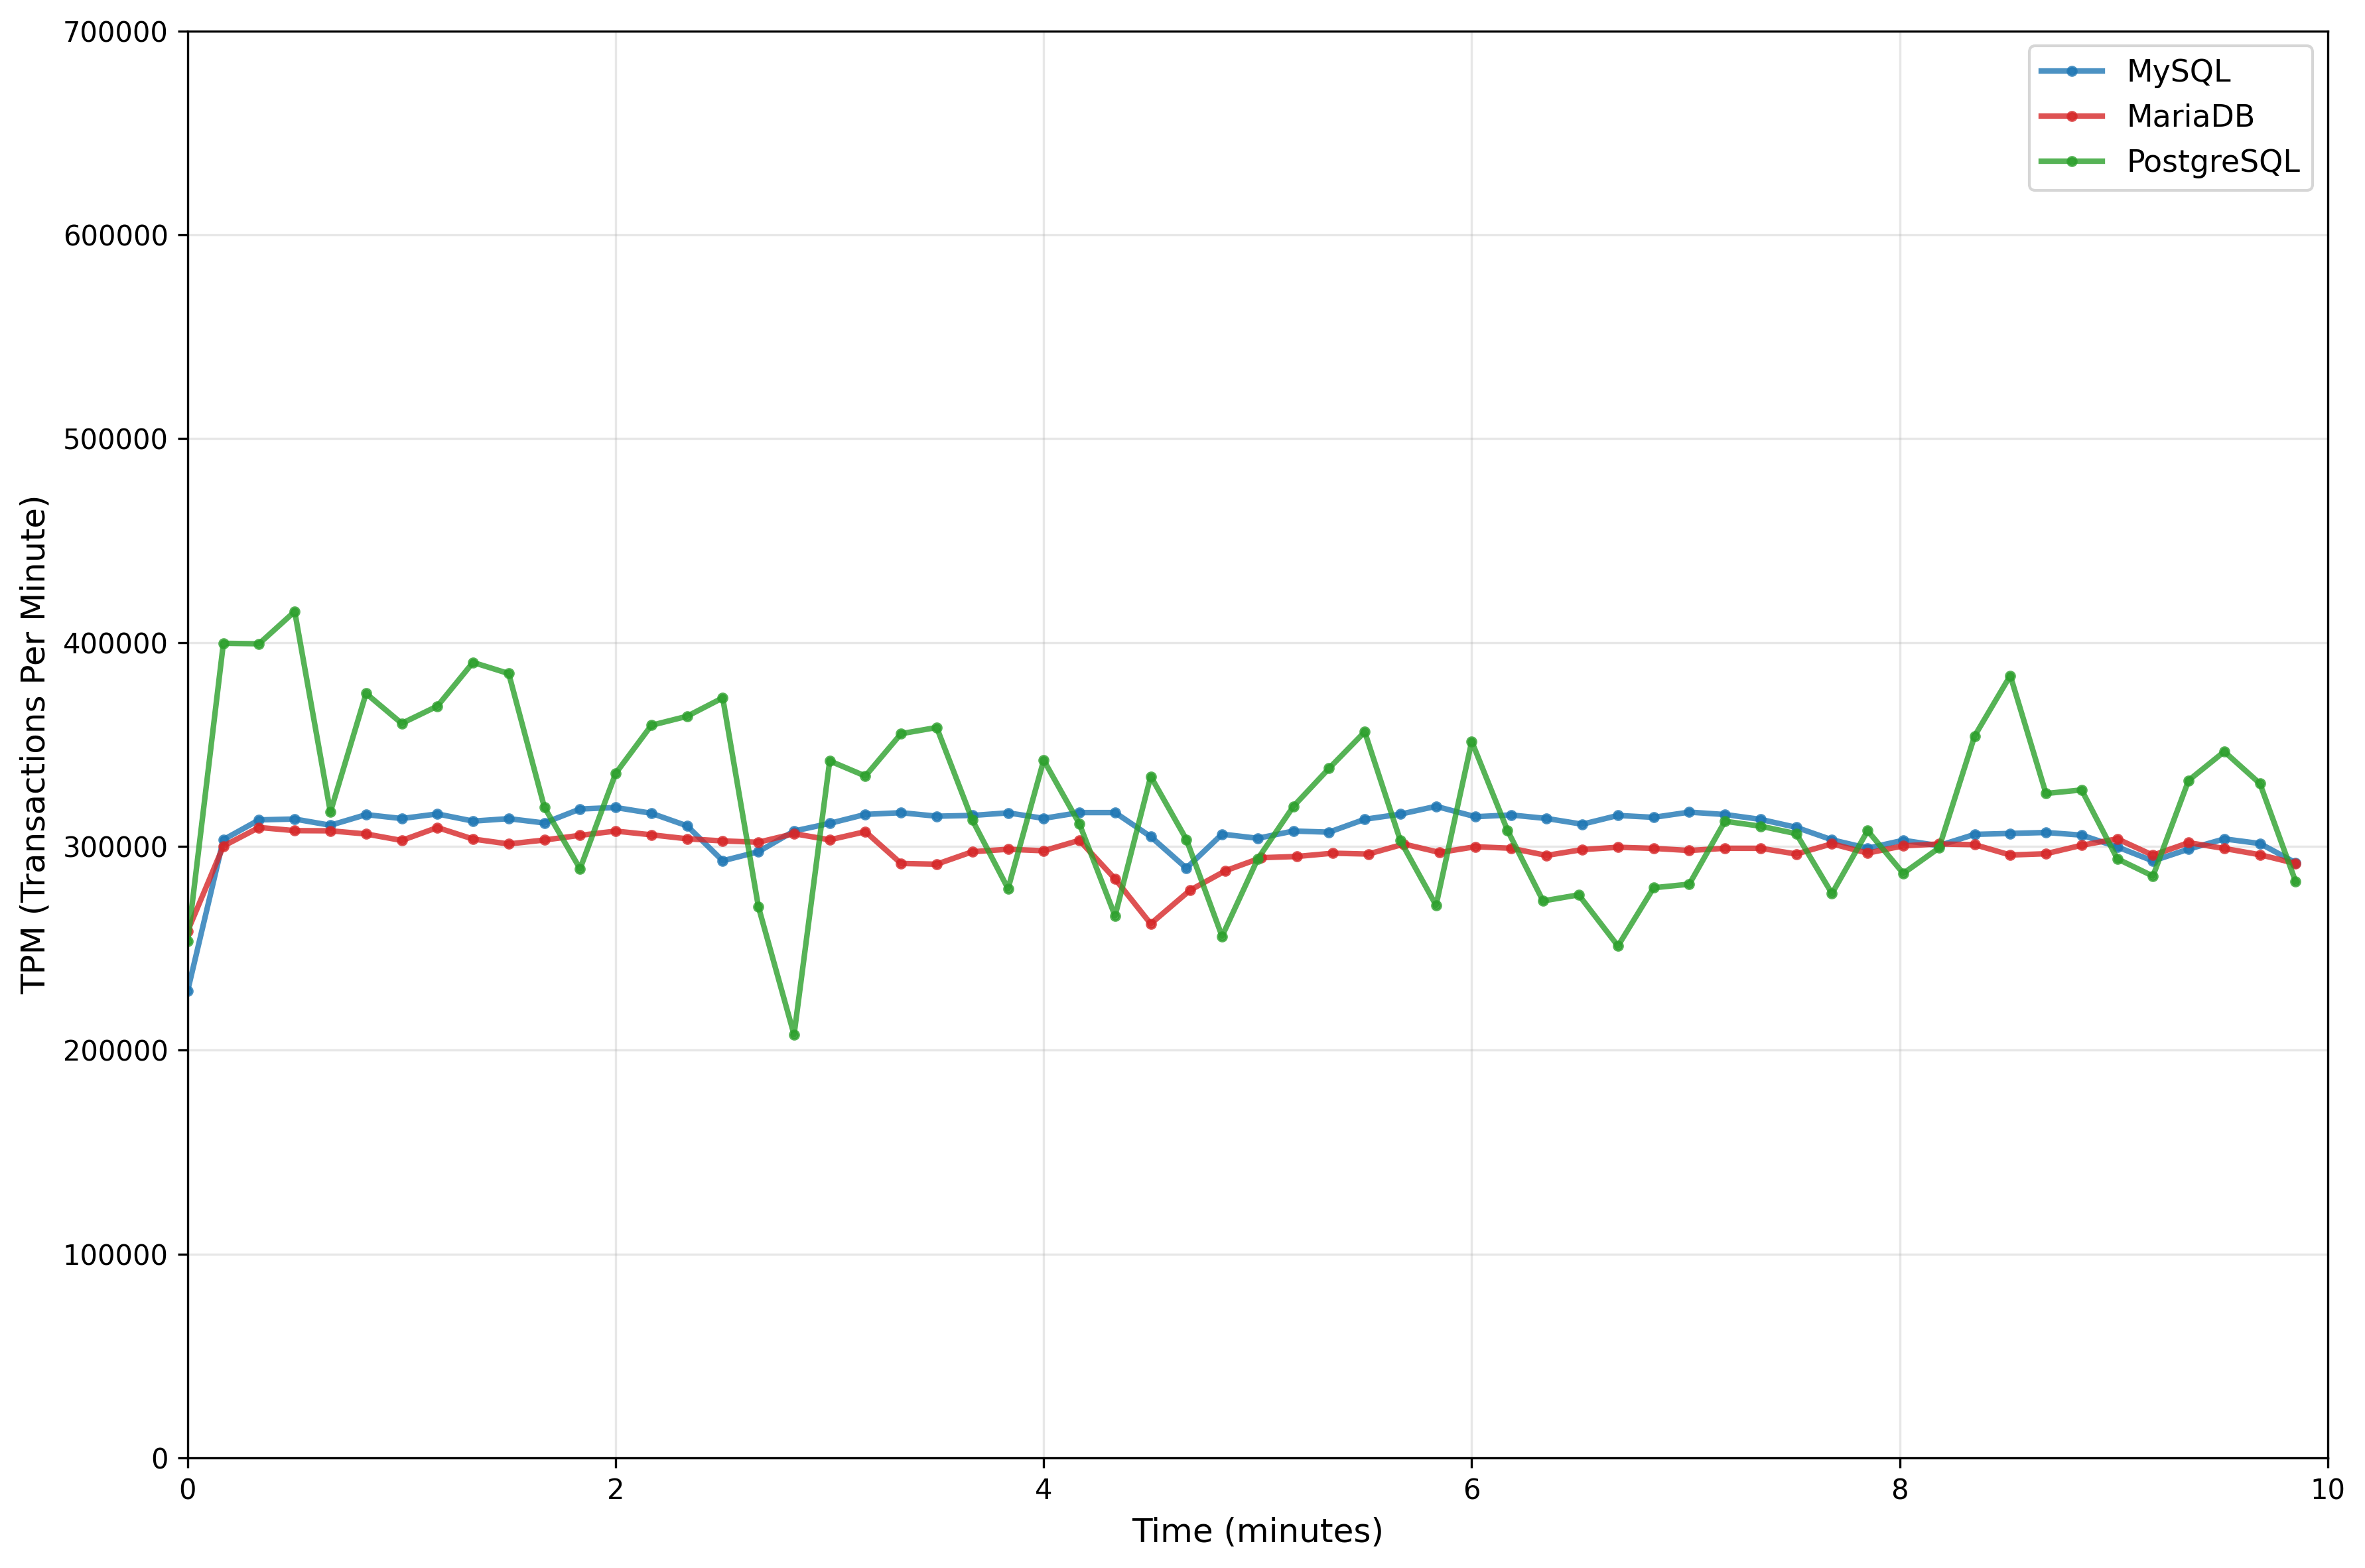
\includegraphics[width=\linewidth]{Images/db_comparison_12_users.png}
        \caption{Database results with 12 Virtual Users}
        \label{fig:db-12vu}
    \end{subfigure}

    \caption{Performance of all Databases for PC 4, with different numbers of virtual users}
    \label{fig:final-all}
    
\end{figure}

This graphs show the differences between the three databases with varied concurrency levels: 2, 4, 8 and 12 Virtual Users (VUs) using \textbf{\hyperref[tab:hardware-setup]{PC 4}}.\\

As the previous benchmarks indicated, PostgreSQL continues to be the top-performing database, achieving the highest average TPM across most test scenarios. While MySQL and MariaDB demonstrate more consistent transaction rates, PostgreSQL delivers significantly higher peak throughput—the peak TPM recorded in Figure \ref{fig:db-4vu} is the highest observed across all tests, which was unexpected.\\

Interestingly, despite overall consistency across machines, this particular benchmark revealed a performance decline for PostgreSQL at 12 Virtual Users  (Figure \ref{fig:db-12vu}). While this is likely influenced by the Apple M1’s 8-core architecture, it also suggests that PostgreSQL does not handle the increased concurrency load as effectively as MySQL or MariaDB, which maintained steadier performance under the same conditions.

\newpage
\section{Discussion}
\label{sec:discussion}

The benchmark findings in this study carry useful data on how MySQL, PostgreSQL and MariaDB perform when subjected to TPROC-C workloads, which simulate atual online transaction processing (OLTP). The test setup was closely planned with identical configurations (where feasible), and changing concurrency levels.

PostgreSQL proved to be the most consistently performing DBMS. The architectural merits of MVCC, lightweight connection handling and a sophisticated query planner enabled it to scale very well with the number of virtual users. Event at high concurrency and distributed warehouse access, PostgreSQL reported higher TPM and NOPM figures than its competitors.

MySQL performed well, with particularly good results at moderate concurrency. The InnoDB storage engine, after being properly tuned, provided good scalability and transactional efficiency. It started to stagnate at full concurrency, indicating some contention or design limitation, but still in high regard as a general-purpose database management system.

MariaDB, while being a fork of MySQL, lagged behind on many test cases. Despite tuning optimizations, it could not keep up with MySQL under load, possibly due to differing implementations or handling of storage engines. It performed well under light workloads but showed saturation and lack of efficiency at high concurrency levels.

\section{Conclusions}
\label{sec:conclusions}

This study presents experimental performance comparison of PostgreSQL, MySQL and MariaDB with simulated OLTP workloads using TPROC-C benchmarks. The results are as follows:

\begin{itemize}
    \setlength\itemsep{0.1em}
    \item PostgreSQL performs the best in both throughput and scalability. It is particularly well suited to the demands of complex transactional systems with high concurrency.
    \item MySQL is also a strong candidate, offering competitive performance for most workloads, especially read-heavy or moderately concurrent workloads. 
    \item MariaDB delivered performance very similar to MySQL, as expected. Interestingly, it appears to benefit slightly more from faster storage. This can be observed by comparing the results in Figures\ref{fig:all-wh} and\ref{fig:mariadb-all}: in the former, where the test was run on a slower SSD, MariaDB performs slightly below MySQL; in the latter, which uses a faster SSD, MariaDB matches or slightly outperforms MySQL. This suggests that MariaDB may be more sensitive to disk speed, potentially due to differences in how it handles I/O or manages internal buffers.
\end{itemize}

Generally speaking, PostgreSQL is recommended for high-performance OLTP workloads requiring concurrency and consistency. MySQL is always a good and efficient choice and MariaDB is a better fit for less complicated situations or MySQL compatibility-oriented environments with less expected load.
